\documentclass[a4paper,oneside,12pt]{book}
%----------------------------------------------------------------------------------------
%	WELCOME!
%   It's probably worth having a read through this file to set up the broad parameters.
%----------------------------------------------------------------------------------------

%----------------------------------------------------------------------------------------
%	COVER PAGE
%   The cover page is laid out in title/title.tex. You can choose a colour
%   or black and white logo
%----------------------------------------------------------------------------------------

%----------------------------------------------------------------------------------------
%	THESIS INFORMATION
%   Put title, author name, degree, type of work, school, department in here
%   It will be used for the title page and for the embedded PDF information
%----------------------------------------------------------------------------------------

\newcommand{\thesistitle}{Network Tomography of Cortical Neuronal Molecular Communication Systems} % Your thesis title, this is used in the title and abstract
\newcommand{\degree}{MAI (Electronic Engineering)} % Your degree name, this is used in the title page and abstract
\newcommand{\typeofthesis}{dissertation} % dissertation, Final Year Project, report, etc.
\newcommand{\authorname}{Peter Mullen} % Your name, this is used in the title page and PDF stuff
%% Comment out the next line if you don't want your ID to appear
\newcommand{\authorid}{14318716} % Your ID
\newcommand{\keywords}{this, that, more} % Keywords for your thesis
\newcommand{\school}{\href{https://www.tcd.ie/eleceng}{School of Electronic and Electrical Engineering}} % Your school's name and URL, this is used in the title page

%% Comment out the next line if you don't want a department to appear
%\newcommand{\department}{\href{http://researchgroup.university.com}{Department Name}} % Your research group's name and URL, this is used in the title page

\AtBeginDocument{
\hypersetup{pdftitle=\thesistitle} % Set the PDF's title to your title
\hypersetup{pdfauthor=\authorname} % Set the PDF's author to your name
\hypersetup{pdfkeywords=\keywords} % Set the PDF's keywords to your keywords
\hypersetup{pdfsubject=\degree} % Set the PDF's keywords to your keywords
}

%% Language and font encodings
\usepackage[T1]{fontenc} 
\usepackage[utf8]{inputenc}
\usepackage[english]{babel}
%\usepackage[numbers]{natbib}

%% Bibliographical stuff
\usepackage[square,sort,comma,numbers]{natbib}

%% Document size
% include showframe as an option if you want to see the boxes
\usepackage[a4paper,top=2.54cm,bottom=2.54cm,left=2.54cm,right=2.54cm,headheight=16pt]{geometry}

%% Useful packages
\usepackage{amsmath}
\usepackage[autostyle=true]{csquotes} % Required to generate language-dependent quotes in the bibliography
\usepackage[pdftex]{graphicx}
\usepackage[colorinlistoftodos]{todonotes}
\usepackage[colorlinks=true, allcolors=black]{hyperref}
\usepackage{caption} % if no caption, no colon
\usepackage{sfmath} %use sans-serif in the maths sections too
\usepackage[parfill]{parskip}    % Begin paragraphs with an empty line rather than an indent
\usepackage{setspace} % to permit one-and-a-half or double spacing
\usepackage{enumerate} % fancy enumerations like (i) (ii) or (a) (b) and suchlike
\usepackage{booktabs} % To thicken table lines
\usepackage{fancyhdr}
\usepackage{wrapfig}
\usepackage{textgreek}
\usepackage{helvet}
\pagestyle{plain} % Embrace simplicity!
\usepackage{listings}
\usepackage{color}
%\usepackage{subfigure}
\usepackage{subcaption}
 
\definecolor{codegreen}{rgb}{0,0.6,0}
\definecolor{codegray}{rgb}{0.5,0.5,0.5}
\definecolor{codepurple}{rgb}{0.58,0,0.82}
\definecolor{backcolour}{rgb}{0.95,0.95,0.92}
\lstdefinestyle{mystyle}{
    backgroundcolor=\color{backcolour},   
    commentstyle=\color{codegreen},
    keywordstyle=\color{magenta},
    numberstyle=\tiny\color{codegray},
    stringstyle=\color{codepurple},
    basicstyle=\footnotesize,
    breakatwhitespace=false,         
    breaklines=true,                 
    captionpos=b,                    
    keepspaces=true,                 
    numbers=left,                    
    numbersep=5pt,                  
    showspaces=false,                
    showstringspaces=false,
    showtabs=false,                  
    tabsize=2
}
\lstset{style=mystyle}

%% The Mechanical engineers require your name and ID on the top of every page.
%% Uncomment the following block if you want your name and ID at the top of
%% (almost) every page.

\pagestyle{fancy}
\fancyhf{} % sets both header and footer to nothing
\renewcommand{\headrulewidth}{0pt}
\cfoot{\thepage}
\ifdefined\authorid
\chead{\it \authorname\ (\authorid)}
\else
\chead{\it \authorname}
\fi
% End of block

%% It is not a requirement of the university that the font should be sans-serif, but
%% the Mechanical engineers require it. Comment out the following line to disable it
%\renewcommand{\familydefault}{\sfdefault} %use the sans-serif font as default
\setlength{\parskip}{10pt}
%% If you're not using sans-serif, consider using Palatino instead of the LaTeX standard
%\usepackage{mathpazo} % Use the Palatino font by default if you prefer it to Computer Modern

\renewcommand{\theequation}{\arabic{equation}} %% use continuous equation numbers

%% Format Chapter headings appropriately
\usepackage{titlesec}
\titleformat{\chapter}[hang] 
{\normalfont\huge\bfseries}{\thechapter}{1cm}{} 

\title{\thesistitle}
\author{\authorname}

\frontmatter
\begin{document}
\begin{titlepage}

\center % Center everything on the page

%% All the text parameters should be taken from the start of the main.tex file.
%% You should only alter stuff here if you want to change the layout

%----------------------------------------------------------------------------------------
%	LOGO SECTION
%----------------------------------------------------------------------------------------
%% Choose one of the following -- a colour or black-and-white logo


\includegraphics{00-Title/Trinity_RGB_transparent_main.png}\\[1cm] 
%
\includegraphics[width=12cm]{title/black-stacked-trinity.jpg}\\[1cm] 

\Large \school\\[1.5cm] % Minor heading such as course title
\ifdefined\department
\large \department\\[1.5cm] % Minor heading such as course title
\fi

%----------------------------------------------------------------------------------------
%	TITLE SECTION
%----------------------------------------------------------------------------------------
\makeatletter
{ \huge \bfseries \thesistitle}\\[1.5cm] % Title of your document
 

%----------------------------------------------------------------------------------------
%	AUTHOR SECTION
%----------------------------------------------------------------------------------------

\ifdefined\authorid
\authorname\\ % Your name
\authorid\\[2cm] % Your Student ID
\else
\authorname\\[2cm] % Your name
\fi

%----------------------------------------------------------------------------------------
%	DATE SECTION
%----------------------------------------------------------------------------------------

{\large \today}\\[2cm] % Date, change the \today to a set date if you want to be precise

 
%----------------------------------------------------------------------------------------
%	TYPE OF THESIS SECTION
%----------------------------------------------------------------------------------------
 A \typeofthesis\ submitted in partial fulfilment\\of the requirements for the degree of\\
\degree

\vfill % Fill the rest of the page with whitespace

\end{titlepage}
\pagenumbering{roman}
\section*{\Huge{Declaration}}
\vspace{1cm}
I hereby declare that this project is entirely my own work and that it has not been submitted as an exercise for a degree at this or any other university.

\vspace{1cm}
I have read and I understand the plagiarism provisions in the General Regulations of the University Calendar for the current year, found at \url{http://www.tcd.ie/calendar}.
\vspace{1cm}

I have also completed the Online Tutorial on avoiding plagiarism `Ready Steady Write', located at
\url{http://tcd-ie.libguides.com/plagiarism/ready-steady-write}.
\vspace{3cm}

Signed:~\rule{5cm}{0.3pt}\hfill Date:~\rule{5cm}{0.3pt}

\chapter*{Abstract}

With the proposal of numerous brain-machine interfaces offering data measurement
of cortical information through minimally-invasive means comes the need for a better
understanding of the circuit-level characteristics of these neuronal systems. These
devices allow data access at a level that can bridge the gap between biological
neuronal analysis and classical communication theory that has been developed for
and applied to man-made network systems.\\
\par
In this investigation we study the application of classical communication theory  in the
biological domain, investigating how network tomography could be
achieved with cortical neuronal circuits. This work involves the simulation of
various neuronal circuits, extraction of the simulated data, and the analysis of this data to develop a
classifying model to infer internal network characteristics based on the measured
endpoint data. Through the processing of the observed data into probabilistic models, we investigate
the use of information theory in cell-to-cell links, and find limitations in the application of
digital mutual information analysis in the biological domain. We investigate the use of simple cross-correlation methods for estimating the synaptic delay in a neuronal circuit, achieving a correlative R-squared score of 0.55.
We also separately train a number of classifiers to identify
the specific cell type (and sub-group types) from input-output voltage measurements, achieving accuracies of up to 70\%.\\
This research can help to advance the next generation of brain-machine interfaces by improving our current understanding of these circuits and the constraints that may come with the application of existing telecommunicative theories in this biological domain.

\newpage
\onehalfspacing%\raggedright %\raggedright turns off justification and hyphenation
%\doublespacing

\section*{\Huge{Acknowledgements}}

I would like to extend my sincerest thanks to all those who have supported and guided me throughout the process of this project.
\par
I would like to firstly thank my supervisor Dr. Nicola Marchetti and co-supervisor Dr Michael Barros for introducing me to the project and for giving me their time, advice, and expertise throughout the year.
\par
Thanks also to my friends and family who made it possible with their support and guidance while undertaking the project.
\par
My sincerest gratitude to Imogen for her unwavering encouragement and patience.

\newpage
\tableofcontents
\listoffigures
\listoftables
\newpage
\section*{\Huge{Acronyms}}
\begin{tabular}{lp{9cm}l}
    AMPA & \textalpha-amino-3-hydroxy-5-methyl-4-isoxazolepropionic \\
    BBP & Blue Brain Project \\
    cAD & Continuous Adapting \\
    CSV & Comma-Separated Value \\
    E-type & Electrical type \\
    FIR & Finite Impulse Response \\
    GMM & Gaussian Mixture Model \\
    HOC & High-Order Calculator \\
    JSON & Javascript Object Notation \\
    LNP & Linear-Nonlinear-Poisson \\
    M-type & Morphological type \\
    NN & (Artificial) Neural Network \\
    NMDA & N-Methyl-D-aspartate \\
    PMF & Probability Mass Function \\
    ROC & Receiver Operating Characteristic \\
    RMS & Root-Mean Square \\
    STA & Spike-Triggered Average \\
    SVM & Support Vector Machine \\
    XML & Extensible Markup Language \\
    
\end{tabular}
\vspace{2cm}


\mainmatter
\chapter{Introduction}

Several brain-machine interfaces have been proposed in recent years which aim to offer measurement of cortical information through minimally-invasive means. With the introduction of such data measurement techniques comes the need to further our understanding of the circuit-level characteristics of these neuronal systems such that the available data can be adequately utilised. The devices will allow access to information of neuronal networks at a level similar to that available from the analysis of man-made network systems, bridging the gap between biological neuronal analysis and classical communication theory that has been developed for, and applied to, these existing network systems \cite{mBarrosMolCom}.\\
The main aim of this project is to investigate the application of existing communication theory in the biological and neuronal domain, specifically in cortical neuronal circuits. Building a model based on this existing theory and machine learning techniques, we aim to infer internal network characteristics and classify cell types from limited endpoint data which could be measured through minimally-invasive approaches in the future, such as the Neural Dust proposed by researchers in the University of Berkeley \cite{NeurDust}. While these physical data measurement techniques are not yet mature enough to be used in practice, existing tools such as the NEURON simulation software from Yale can generate accurate simulated data based on known cell types, similar to the form of data which will be measurable by the aforementioned physical devices \cite{NEURON}.The data obtained from this software can then be processed through mathematical software such as Matlab or data-mining software such as RapidMiner, which offers a powerful environment for developing data processing and machine learning models \cite{rapidMiner}. By integrating and defining an interface between NEURON, Matlab, and RapidMiner, we obtain the framework needed to simulate the communication between biological neurons and to analyse it through machine learning techniques.
\par
One of the primary goals of this project is to investigate the classification and inference of neuronal circuits, especially at an inter-layer scale and with a larger variety of cell-types, progressing the field towards classification of more complex cortical circuits.\\
In this study, we investigate the effect of signal propagation in the circuits, and attempt to quantise the level of information communicated between cells. The data generated by the NEURON tool represents the signals as they exist in an ideal network, and so we investigate the effects that cell-to-cell connection parameters may have on the ability for the cells to transfer information between each other. To this end, we investigate the application of digital forms of information theoretic models in the biological domain, and find limitations in the insight that these models may provide in this setting.\\

We also investigate the use of classification algorithms in the analysis of various forms of cortical networks (either from known networks \cite{bbpTop} or using algorithmically driven approaches \cite{reimann2015algorithm}. One requirement in the use of such classifiers is the need to reduce the dimensionality of the measured data. This is done through feature extraction, which can also be applied to the neural network and decision tree models to improve performance. We therefore attempt to characterise the response of individual neural cells in a finite dimension space. Through the use of characteristic models and integration with high-performance classifiers, we develop a classification system to predict cell type (and sub-group type) based entirely off input-output voltage measurements.\\

\par

Finally, we investigate the use of the classification models trained on the data from the previous step in the application of network tomography to reconstruct the cell-types in a known topology based on endpoint measurements taken around the network.\\
The project aims can therefore be summarised as the following objectives:
\begin{itemize}
    \item Construct and simulate a number of cortical circuits in NEURON, extracting data for each circuit.
    \item Using existing models in the domain of information theory, analyse the entropy and mutual information of cell-to-cell connections.
    \item Using Matlab and RapidMiner, construct models to investigate the application of cell-characterisation models to extract features from the endpoint measurements for the training of a number of classification algorithms.
    \item Investigate the application of the trained classification model to predict unknown cell-types from the endpoint measurements of a cortical network.
\end{itemize}


\section{Outline of Proceeding Chapters}

The proceeding document is laid out as follows. In Chapter \ref{chap:back}, \emph{Background}, we cover the supporting theory of the topics and domains relating to the experimentation and investigations conducted in the course of this study, such as the biological theory of neurons and neuronal circuits, the theory and application of network tomography, the concept of information and information theory, and finally a comparison of the functionality of various classification algorithms. In Chapter \ref{chap:relWork}, \emph{Related Work}, we review studies related to the work carried out in this investigation, comparing the methods in which the work was conducted and the results found. In Chapter \ref{chap:meth}, \emph{Methodology} we describe the steps taken to carry out the experiments conducted in the various experiments, including a complete description of the supporting tools and frameworks used, as well as the methods in which the generated data was processed into usable information. In Chapter \ref{chap:res}, \emph{Results}, we present and describe the results generated from the experimentation and analysis. In Chapter \ref{chap:disc}, \emph{Discussion and Future Work}, we discuss the generated results, comparing our results with those of the related work and discussing the reasoning behind any differences between the two, while also suggesting potential future work that could improve on our investigation. Finally, we conclude in Chapter \ref{chap:conc}, \emph{Conclusion}, with a summary of the contributions and findings of the investigation.


\chapter{Background}
\label{chap:back}
\section*{Chapter Outline}
In this chapter we cover the background theory of the various domains which relate to the investigations carried out in this study. We first describe basic theory on the formation, operation, and classification of neuronal cells, how individual cells interconnect to form networks, and how the cells can be characterised using mathematical models. We then describe the theory of network tomography and how it is applied in existing communication networks. Finally, we explain the operation of several classification algorithms and compare their operation.

\section{Neurons and Cortical Circuits}
\label{chap:back:neurons}
% Information on the basics of neuronal cells from the bottom up. Basically a quick overview of everything from molecular communication and synaptic messages to cellular response, morphology etc and onto cortical networks.\\
% Also some information here on LNP models and other ways of characterising neurons.
% \begin{itemize}
%     \item Overview of neuronal cells (intro basically).
%     \item Electrical Characteristics of the signals
%     \item How the electrical signal is "encoded" as electro-chemical processes
%     \item How the electro-chemical process relates to the synapse + cell body
%     \item Describe the e-type differences between cells
%     \item More info on synaptic connections (types, number, neurotransmitters etc)
%     \item Info on m-types of cells. 
%     \item Describe the LNP-cascade model of cell characterisation
%     \item Info on interconnecting cells into a network
%     \item Some info on types of cell networks and how they arrange into layers
%     \item Finish with info on the specific types of above theory that we deal with (layers, mTypes, eTypes, synaptic types and topologies.
% \end{itemize}

A neuron is a type of cell present in the body of most multicellular organisms, differentiated from other biological cells by its ability to be stimulated by an electrical signal, responding in kind with an electrical signal which can be used to excite further neurons. Neurons have multiple roles, with sensory neurons providing sensory input from the organisms environment (light, sound, etc.) and delivering this input to the brain where a different set of neurons form a complex neural network in order to process the sensory input, responding appropriately. Response signals from the neurons of the brain are carried to various parts of the body such as muscles through motor neurons, allowing the organism to physically respond to the environmental sensory input. These different neuronal cells work together to form the nervous system which allow the organism to have contextual awareness of the environment. \par

In this study, we deal solely with the neurons found in the brain; specifically, the neurons investigated are based on prior research into the neurons of the somatosensory cortex of a juvenile rat. This segment is found in the the outer portion of the cerebrum of the brain, referred to as the neocortex. The neocortex is typically treated as being a tightly-packed system of vertical structures (cortical columns), and classified into 6 interconnected horizontal layers. The neurons in this investigation are based on data retrieved from a single cortical column, each classified by layer and a number of other properties discussed later.
\par
While different neurons may have separate roles in the body, the basic form of each neuron is typically made of three sections: the dendrites, the soma, and an axon. An illustration of the layout of a typical neuron is shown in Figure \ref{neuronOverview}. A branched system of dendrites act as an input carrying the electrical signals to the soma (the cell body) which houses the cell nucleus and generates an output signal as some function of the input signals. The output signal is then carried away from the soma by the axon which may then branch, passing the electrical signal onto the dendrites of further cells.\\

\begin{figure}
    \centering
    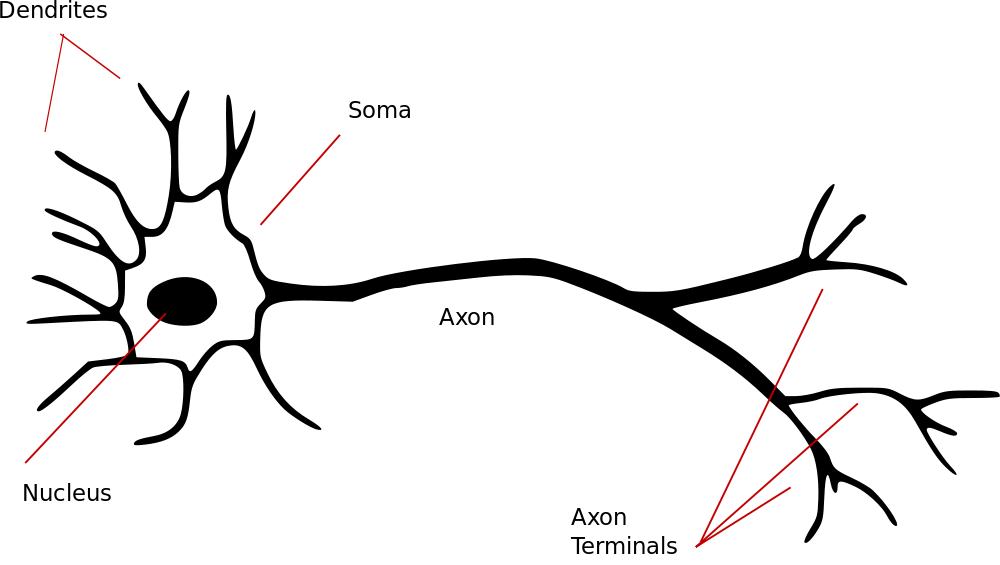
\includegraphics[width=0.75\textwidth]{02-Background/neuron_annotated.png}
    \caption{ Annotated illustration of a typical neuron \cite{neuronAnnotated} showing the branched dendritic tree as input, cell body (soma), and axon as output }
    \label{neuronOverview}
\end{figure}

\par

The axon and subsequent dendrite are generally not directly connected, rather the electrical signal is passed through an electro-chemical interface referred to as a \emph{synapse}. For a given synaptic connection, the neuron acting as a signal source is referred to as the \emph{pre-synaptic cell} while the neuron acting as the signal receiver is referred to as the \emph{post-synaptic cell}. A single pre-synaptic cell may connect to multiple post-synaptic cells, and similarly a post-synaptic cell may receive electrical stimulation from multiple pre-synaptic cells.
\begin{wrapfigure}{R}{0.5\textwidth}
  %  \centering
    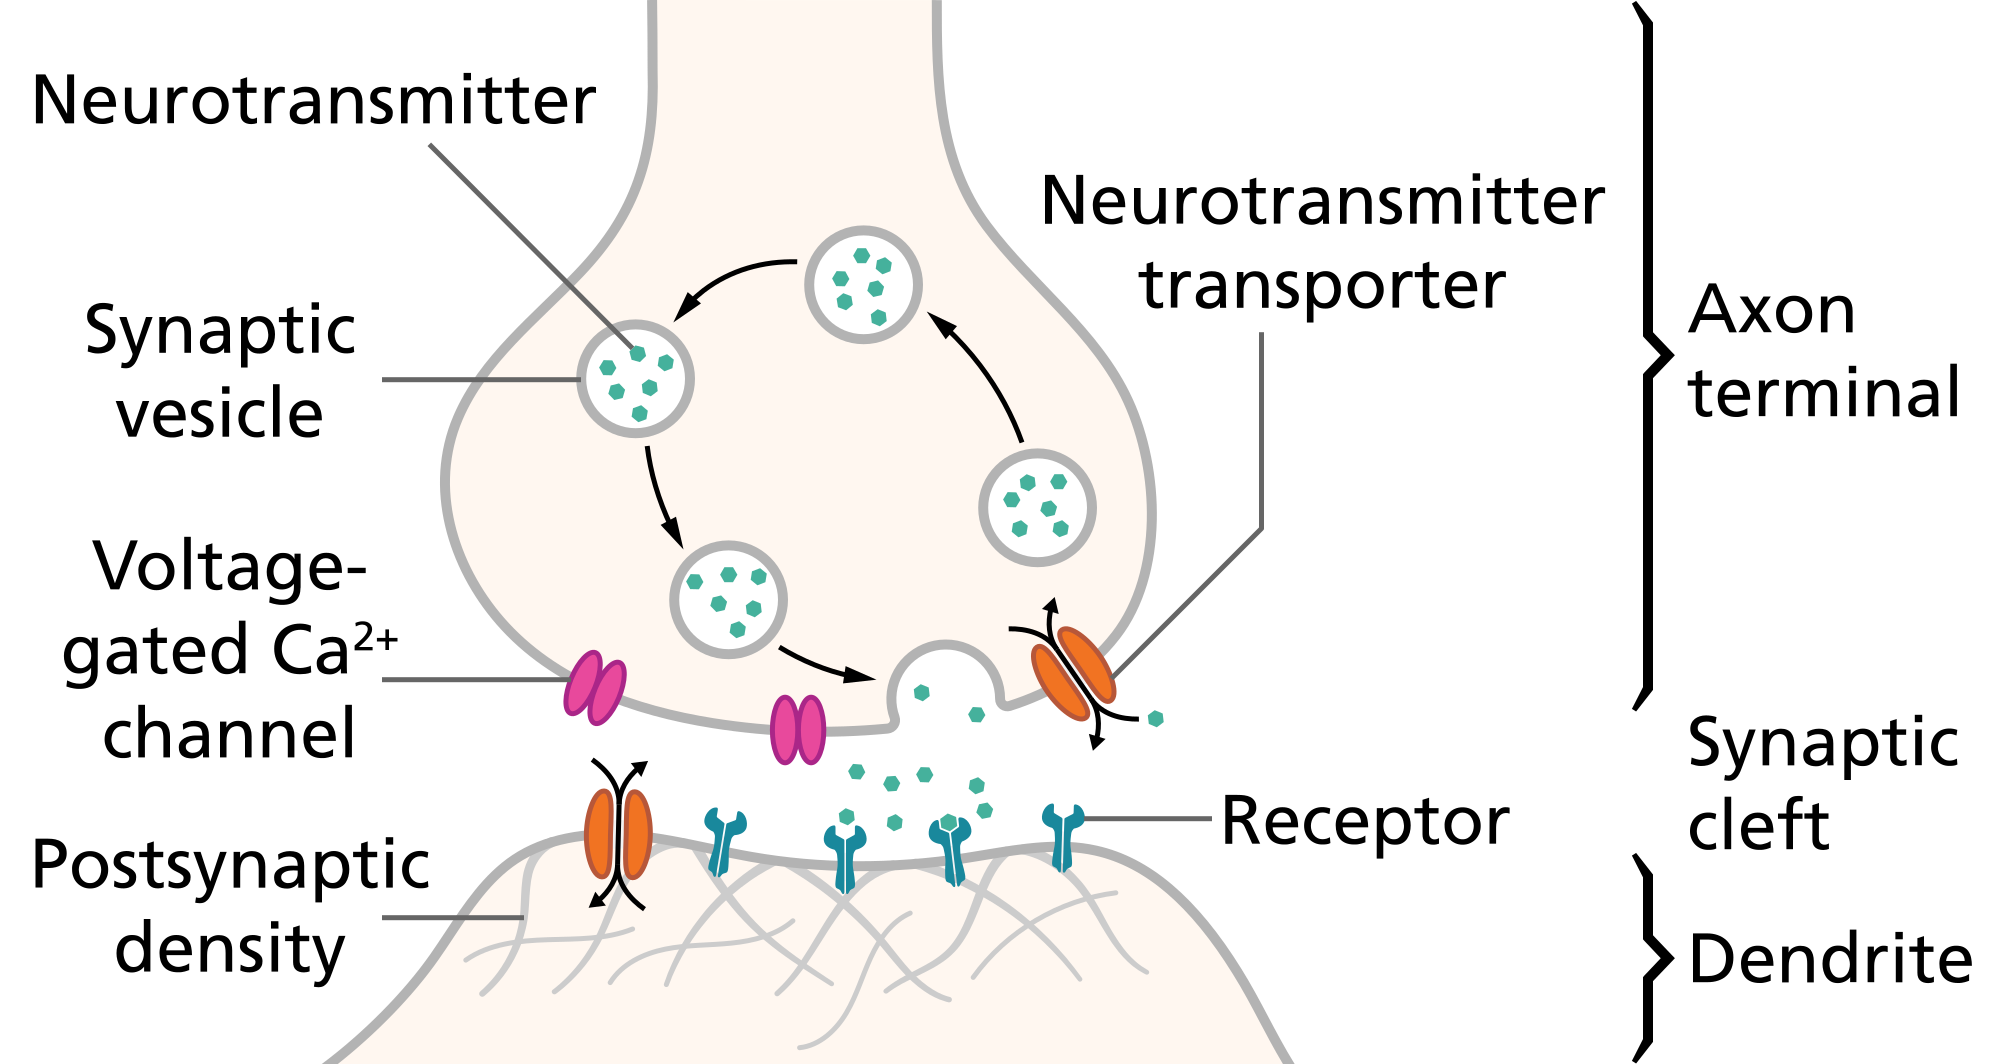
\includegraphics[width=0.5\textwidth]{02-Background/synapse.png}
    \caption{Illustration of synaptic operation \cite{synapseAnnotated} demonstrating the release of neurotransmitters from axon terminal, binding to receptors on opposing dendrite  }
    \label{synapseOverview}
\end{wrapfigure}
As the electrical signal propagates through the axon and arrives at an axon terminal, voltage-gated calcium (Ca\textsuperscript{2+}) channels in the terminal are activated, which causes the release of a \emph{neurotransmitter}, a class of chemical which travels across the synaptic cleft and binds to a receptor at the dendritic receiver. The binding of the neurotransmitter to the receptor elicits some form of response in the post-synaptic cell. The neurotransmitter may cause electrical stimulation in the case of an \emph{excitatory} neurotransmitter, causing a signal to propagate through the dendrite towards the post-synaptic soma, or the neurotransmitter may inhibit the production of an electrical signal in the case of an \emph{inhibitory} neurotransmitter. The neurotransmitter is generally present in the synaptic cleft for a short period of time before it is all bound to receptors, metabolised, or returned to the axon terminal in a process referred to as reuptake.  An illustration of this electro-chemical synaptic process, as well as the general form of a synapse, is shown in Figure \ref{synapseOverview}. The ability for the neuronal system to encode signals (and therefore information) in single molecules such as Ca\textsuperscript{2+} leads to the concept of \emph{molecular communication}, which is the study of this process and how nano-technology may interface with biological components for robust machine-neuron interfaces \cite{mBarrosMolCom}.
\par

While the general form of neurons is consistent, there are a number of properties and classifications used to differentiate between cells to better group them by their input-output response characteristics. In this investigation we classify the individual neurons by neocortical layer, by morphological-type (m-type), and by electrical type (e-type). The m-type of a cell describes its physical properties such as shape, size, and structure. Different m-types exist in different proportions between layers. An overview of the m-types present in the data-set used in this investigation is shown in Figure \ref{mtypeOverview}. The e-type of a cell describes its electrical characteristics which in turn describe how the soma responds to incoming stimulating signals (continuous, burst, delay, etc.). In the neuronal dataset used in this study, the most common e-types are \emph{Continuous Accomodating} (cAC), \emph{Continuous Non-Accomodating}(cNAC), and \emph{Delayed Non-Accomodating}(dNAC), while e-types such as \emph{Continuous Stuttering}(cSTUT) and \emph{Burst Irregular}(bIR) are less common \cite{reconSim}. A complete list of the m-types and e-types in the dataset are tabulated in \ref{tab:m-type_table} and \ref{tab:e-type_table}, respectively.
\begin{figure}
    \centering
    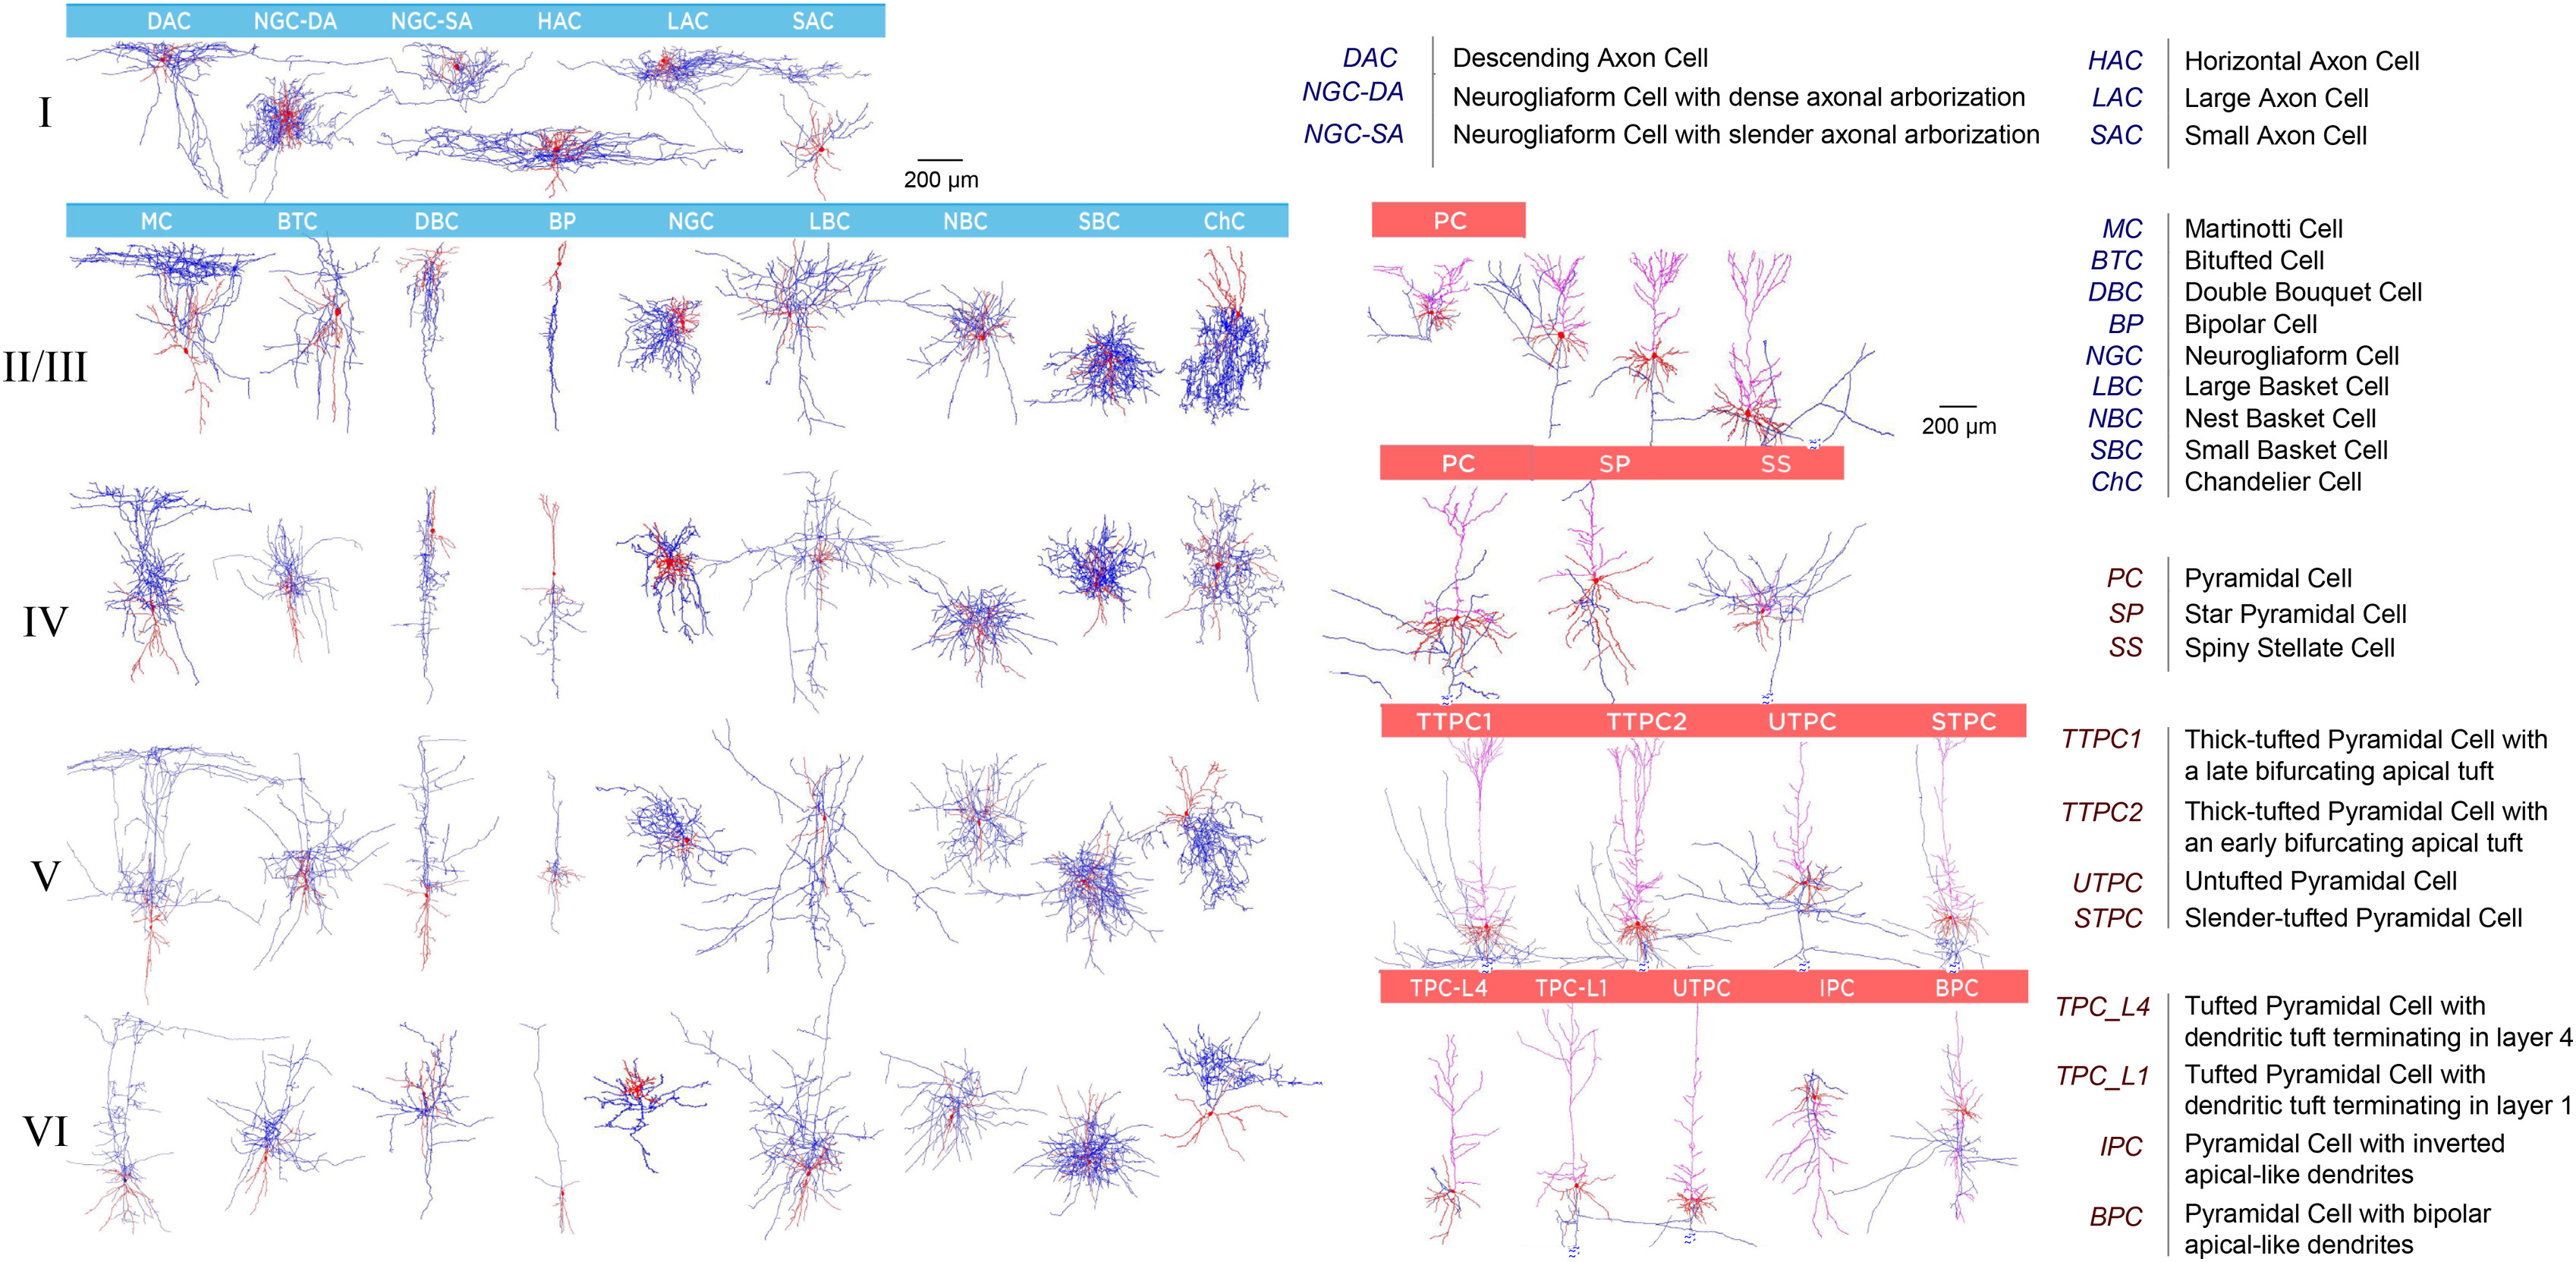
\includegraphics[width=\textwidth]{02-Background/mtypes.jpg}
    \caption{Table of neocortical neuronal morphologies \cite{reconSim} as they appear in each layer. Axons shown as blue, and dendrites as red.}
    \label{mtypeOverview}
\end{figure}

\par

The connection between neurons leads to the emergence of complex neural networks. While the brain as a whole is one large network, there are a number of smaller network topologies that are found across the brain \cite{bbpTop}. These small-world topologies can exist across neocortical layers and they tend to present with similar cell-types. For example, in-hub topologies tend to be formed by excitatory pyramidal cells residing within layers 5 and 6, while out-hub topologies are formed by a mix of inhibitory and excitatory neurons in layers 4 to 6. The "connection probability" between any 2 cells (i.e. the probability of such a connection being observed) is not equal for all cell-pairs. Along with a connection probability, each cell-to-cell pathway has a certain statistical distribution for various connection parameters such as number of synapses in the connection, the type of synaptic connection, cell-separation distance etc. \cite{bbpTop}. These statistical distributions can be used to construct arbitrary network topologies \emph{in silico} and associate a corresponding probability of real-world occurrence. 

\par

Of major interest to us in this investigation is the characterisation of the signals propagated through and between neurons. The response of a neuron is of the \emph{all-or-none} principle; that is, the cell will either respond fully or will not respond at all. The response takes the form of a voltage spike, and the response over time is characterised as a spike train. A sample time-voltage plot from the measurement of the soma-membrane voltage of a simulated neuron is shown in Figure \ref{image:sampleSpike}. As the release of neurotransmitters in the synapse is a response of a spike event rather than of the small variations in resting potential, the response of a post-synaptic cell is therefore also a function of the spike events. Analytically, the spike events are treated in a probabilistic fashion (i.e. the probability of a spike occurring)  to which a Poisson process fits well. The Poisson process describes a model for the estimated time between events, and so when applied in this domain to estimate the time between voltage spikes, the intercellular signals are seen as a \emph{Poisson Spike Train}. This has a number of useful implications for the analysis of these intercellular signals in that the probabilistic modelling of the signal allows for the application of the Poisson model in telecommunicative domains that rely on signal probabilities, such as mutual information and channel capacity. Another implication of this spike-triggered-event property is that the cell can be described as a time-varying process responding to (and with) an impulse train. One such model commonly used is the \emph{Linear-Nonlinear-Poisson cascade}(LNP) model \cite{lnp}.
\par
The LNP model consists of three serial components: a linear filter, a non-linear transform, and a Poisson spike-generating process. This model is typically used to characterise the neurons in the visual system, and so the linear filter is used to describe the response of the neuron in both space and time; typically (in the case of a visual system) the input stimulus is a fixed-size screen and so the space component refers to the pixel-position in space. This filter therefore describes the input image-variation over time that is most likely to elicit a response from the cell. The non-linear transform of the model describes the spike-rate (spikes per second) which is then used in the Poisson-process to generate the spike train. This LNP model is one of many models for the characterisation of the spike-response of a neural cell, however one common property between many of them (and the property of interest in this study) is that of dimensionality reduction. When dealing with the voltage-time measurement of a neuron, the dimensionality of the data increases with every timestep. Through the reduction in dimensionality we can describe the characteristics of an individual cell in a lower, fixed number of dimensions, regardless of the number of datapoints measured. In the LNP model, the dimensionality reduction occurs in the linear-filter component (the non-linearity and Poisson component deal mainly with the production of a spike train which is not required here). While this model generally deals with a spatio-temporal input (i.e. an external screen), we can adapt the concept to use the output spike-train of another neuron as input. As the spike-train is essentially an impulse-train, the resulting linear filter that best characterises the neuron can be estimated as the impulse response of a time varying system taking an impulse train as input and generating a continuous voltage-time output. In this case, a finite-impulse response (FIR) filter model was used. The dimensionality of the model is therefore proportional to the number of filter coefficients in the estimated FIR filter which can be significantly lower than the number of timesteps in the measured data. By measuring the input and output spike trains of a single cell, an estimation can be determined of the k-order FIR filter that best characterises the neuron's impulse response.
\begin{figure}[ht]
    \centering
    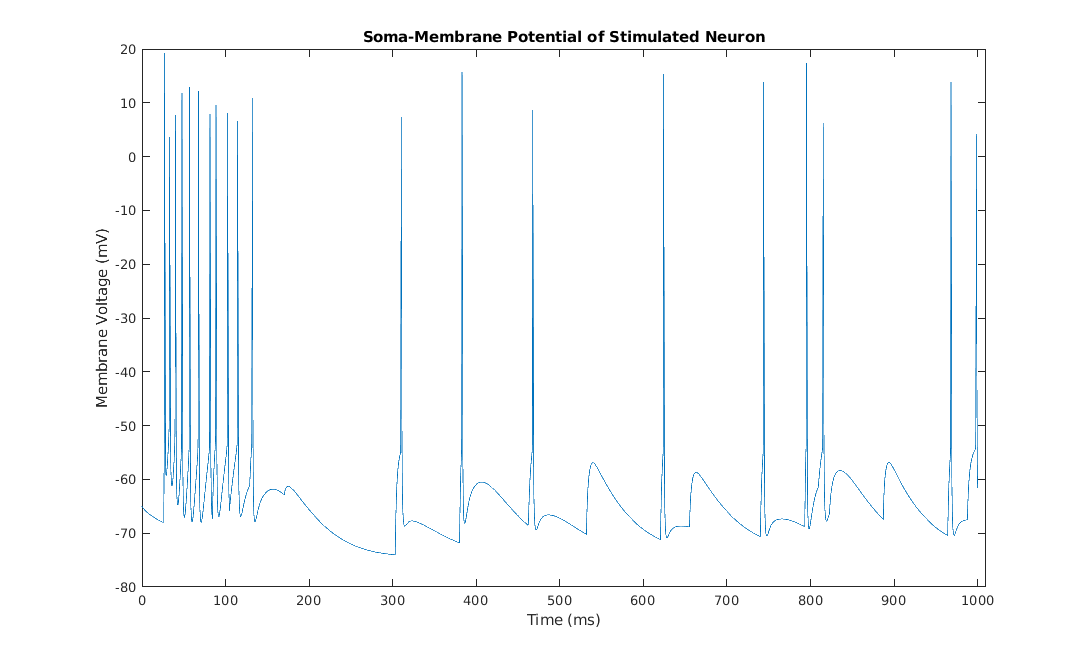
\includegraphics[width=0.75\textwidth]{02-Background/sampleSpikeTrain.png}
    \caption{Spike Train of a Neural Cell}
    \label{image:sampleSpike}
\end{figure}
\par
Previously mentioned was the distinction between excitatory and inhibitory responses. In general, an excitatory neuron is one that increases the spike rate, while an inhibitory neuron is one that decreases the spike rate. This classification is not based on a single cellular property and is instead a result of a number of factors. One such factor is the neuron's e-type. Of the 11 e-types, it was found that only the continuous-adapting (cAD) type was excitatory, while the other types were inhibitory \cite{reconSim}. As well as this, the distinction does not entirely depend on a single cell, but can also refer to the type of synaptic connection between two cells. On the synaptic distinction, the inhibitory/excitatory classification of a given cell is taken from the post-synaptic point of view; that is, if a synaptic connection is inhibitory, then the post-synaptic cell regards the pre-synaptic cell as inhibitory, and vice-versa. This distinction is made more complex by the large number of different synaptic connections (i.e. neurotransmitters/receptors in the synapse). In the dataset used in this study, only 2 synapse-types are provided, differing in receptor/neurotransmitter type. One is inhibitory and is of the GABA class, which responds to the gamma-aminobutyric acid neurotransmitter. The second is excitatory and is made of two neurotransmitter/receptor pairs, one being the N-Methyl-D-aspartate (NMDA) neurotransmitter and the other being the \textalpha-amino-3-hydroxy-5-methyl-4-isoxazolepropionic acid (AMPA) neurotransmitter. \\

\section{Network Tomography}
% Background info from a telecom point of view on the broad scope of network tomography. Discuss different types of tomography (mainly focussing on the types we deal with in the project), as well as how tomography is implemented and used in real-world networks (e.g. internet systems for identifying faults and bottlenecks). Maybe include some of the theory here such as the identifiability of network-level delay using network tomography.
% \begin{itemize}
%     \item Overview of network tomography.
%     \item Describe methods of implementing network tomography (research here)
%     \item Info on how the above methods are used in practice.
%     \item Describe the specific type of network tomography that we use (i.e. basic node-type classification and delay.
% \end{itemize}

Network tomography is a branch of telecommunicative study that deals with the inference of internal network properties from a finite number of endpoint measurements. This concept can be applied in many specific applications, however it is generally used in internet systems to determine link-loss and link-delay characteristics \cite{intTom}. The benefit of this approach is that issues in the network (bottlenecks, broken links etc.) can quickly be identified and located, allowing the service provider to dispatch a small number of engineers to the source of the issue rather than requiring a larger number of engineers across the entire network to manually locate the fault. In these systems, the endpoint data typically comes from measurements at network terminals (e.g. a user's modem) which is then transferred back to the service provider where analysis can be done. Analytically speaking, the problem of broad inference of the entire network can be approximated by describing the measurements as a linear model \cite{intTom} given by:
\begin{equation}
    \label{generalNetTom}
    \vec{y}=\boldsymbol{A}\vec{\theta}+\epsilon
\end{equation}
where $\vec{y}$ is a vector of measurements, $\boldsymbol{A}$ is a routing matrix representing the network node connectivity, $\vec{\theta}$ is a vector of link parameters (delay, loss etc.), and $\epsilon$ is a noise term. The routing network is typically a binary matrix with the $i^{th},j^{th}$ element being 1 to represent a connection between the $i^{th}$ node and the $j^{th}$ node, and 0 representing no connection between the two nodes. The network inference in this case would be estimating the vector $\vec{\theta}$ given some endpoint measurements $\vec{y}$ and knowledge of the networking routing matrix, along with some distribution for the noise parameter $\epsilon$ (Gaussian, Poisson, etc.). For large networks this poses a problem in the computational solution for the linear model, as the dimensionality of $\boldsymbol{A}$ can grow prohibitively large for larger networks. Two options are discussed in \cite{intTom} to solve the linear equation for large networks. One option is to be content with the computational complexity in the linear solution, while the other option is to introduce a regularisation term in order to induce identifiability.
\par
One method of inducing identifiability in link-delay network tomography is through the use of characteristic functions \cite{netTomFour}. The characteristic function of $\vec{y}$ for any I-dimensional $\vec{t}$ is described as
\begin{equation}
    \label{linkDelayCF}
    \phi_{\vec{y}}(\vec{t}) = \prod_{j=1}^{J}\phi_{\vec{\theta_{j}}}(\vec{t}^{T}\boldsymbol{A}^{j})
\end{equation}
where $\phi_{\vec{y}}$ and $\phi_{\vec{\theta_{j}}}$ are the characteristic functions for $\vec{y}$ and $\vec{\theta}$, and $\boldsymbol{A}^{j}$ is the $j^{th}$ column of the routing matrix $\boldsymbol{A}$. The implication of this is that the identifiability problem of the model is satisfied given knowledge of the routing matrix and the characteristic function of the measured data.

\par

There are a number of differences between the networks generally used in network tomography (i.e. internet networks) and the cortical networks investigated in this study. Node-to-node links in internet networks tend to be bi-directional such that information can flow in both directions. This is necessary for the TCP data-link protocol in particular for the acknowledgement of the receipt of packets, along with other uses such as the capability of both uploading and downloading data from some server. In cortical circuits, the cell-to-cell links are mostly unidirectional with signals propagating in a single direction. This has a number of implications for the routing matrix $\boldsymbol{A}$, name that the presence of a 1 for element $\boldsymbol{A}_{i,j}$ implies a high probability of a 0 for element $\boldsymbol{A}_{j,i}$.\\
Another difference between the two classes of networks is the presence of defined routing in internet networks, namely the distinction between \emph{unicast} and \emph{multicast} routing. In unicast routing, the concept is to find some path between any two nodes, passing the signal through other nodes on the path. While any node may have a number of adjacent nodes, the signal is passed along only one of the paths. In multicast routing, the signal is propagated on all outbound paths from the node. This multicast routing principle is most similar to the process of signal propagation in cortical networks. As there is no protocol for specifying specific nodes or endpoints in neural circuits, any signal produced by a cell will be passed to all of its synaptic links with adjacent cells. 

\par

While there exists multiple options for the estimation of the network parameters $\theta$ after inducing identifiability, such as expectation maximisation, maximum likelihood, and maximum a posteriori methods, this study deals mainly with smaller, simpler forms of network tomography. Rather than initially focus on large-scale networks, smaller networks are investigated as a first-step approach to find the features and methods for best characterising the lower-level components of the neuronal networks. As well as this, the design and verification of the network tomography for larger networks increases the computational complexity significantly for the signal processing of the large quantities of produced data, and so is out of the scope of this work.

\section{Information Theory}
\label{chap:back:infTheory}
% Some background details on information theory, up to and including mutual information. Discuss uncertainty and the link between the quality of a network channel and the probability of the events transmitted/received.
% \begin{itemize}
%     \item Overview of what information theory is (analysing information)
%     \item Build up from base to mutual information.
%     \item Describe how mutual information is used to obtain channel capacity
%     \item Describe differences between mutual-information models (i.e. different models representing the same idea based on channel type)
%     \item Mention the type of model we'll be looking at and why (and maybe why it's not a great idea)
% \end{itemize}

Information theory is the study of knowledge, quantising the concept of information into mathematically applicable models. The information theory of discrete systems deals largely with symbols and symbol events. As there is a close link between information theory and probability, a symbol can be thought of being similar to a discrete random variable, where a source may produce a symbol at every event from a set of possible symbol values $\{s_{1}...s_{N}\}$. For an equiprobable set of symbols, the probability of each symbol arising from some event is $1/N$, and the information of a source is given by 
\begin{equation}
    \label{eq:infoSymb}
    I = \log(N)
\end{equation}
where I is the information and n is the number of symbols. Generally, a log to the base 2 is used which gives the information unit as number of \emph{bits} expressed by the source. We can also express the information measure in \ref{eq:infoSymb} as a function of the symbol probability; for an equiprobable set of N symbols, each with probability $P = 1/N$, we can adjust the information equation as
\begin{equation}
    \label{eq:infoEquiProb}
    I = \log(N) = -\log(1/N) = -\log(P) 
\end{equation}
where $P$ is the probability of a given symbol.\\
While this expression is useful for equiprobable systems, it does not adequately represent systems where the probability of each symbol is not equal. For example, consider a source with 2 possible symbols. If the probability of symbol $s_{1} >> s_{2}$, then the observation of some symbol does not cause the observer to gain $log_{2}(2) = 1 bits$ of information as the observer had prior knowledge of the probability of the event. This leads to the definition of a source \emph{uncertainty}, as it is more useful to quantify the source as a measure of how uncertain the observer is of the event value. This uncertainty measure takes the probability distribution of the symbol set into account, and is defined by
\begin{equation}
    \label{eq:uncertProb}
    I(s_{k}) = -\log_{2}(p_{k})
   % H(X) = -\sum_{j=0}^{N}p(x_{j})log_{2}(p(x_{j}))
\end{equation}
where $s_{k}$ is some symbol in the symbol set $\{s_{1}...s_{N}\}$ and $p_{k}$ is the corresponding probability of the corresponding symbol occurring. This measure of information gives the number of bits of information gained as a quanta of information from observing some symbol with a given probability.\\
It is useful to extend this definition of information beyond individual symbols to some measure of the uncertainty of a source generating the events. We can therefore take the expected information gained per symbol on observation of the random variable by taking the sum of information gained from each possible symbol (given by Eq. \ref{eq:uncertProb}), weighted by the probability of observing the symbol. This is given by
\begin{equation}
    \label{eq:entropyDiscr}
    H(X) = -\sum_{k=0}^{N}p(s_{k})\log_{2}(p(s_{k}))
\end{equation}
where H(X) is the expected uncertainty of uncertainty of event source $X$, and $s_{k}$ is some symbol in the set $\{s_{1}...s_{N}\}$. This averaged-uncertainty measure is also referred to as the \emph{entropy} of X, and tells us the average number of bits gained through the observation of the random variable X, or alternatively the average number of bits required to describe X.
\par
Another useful metric in information theory is that of \emph{conditional entropy}, or the entropy of some random variable given the knowledge of another random variable. Given the random variable X, the entropy of X given a particular value of another random variable $Y=y_{k}$ is given by
\begin{equation}
    \label{eq:condEntSing}
    H(X|Y=y_{k}) = -\sum_{j=0}^{N}P(X=x_{j}|Y=y_{k})\log_{2}(P(X=x_{j}|Y=y_{k}))
\end{equation}
Summing over all values of Y and weighting by the probability of the symbol $y_{k}$, we get
\begin{equation}
    \label{eq:condEnt}
    H(X|Y) = \sum_{k=0}^{N}H(X|Y=y_{k})p(y_{k}) = -\sum_{k=0}^{N}\sum_{j=0}^{N}p(x_{j},y_{k})\log_{2}(p(x_{j}|y_{k}))
\end{equation}
where $H(X|Y)$ is the conditional entropy of X given Y, $p(x_{j},y_{k})$ is the joint probability of symbols $x_{j}$ and $y_{k}$, and $p(x_{j}|y_{k})$ is the conditional probability of the same symbols.\\
Given this definition of the conditional entropy, we can obtain an expression for the reduction in entropy of X, given some observed event Y. This is defined by
\begin{equation}
    \label{eq:mutualInf}
    I(X;Y) = H(X) - H(X|Y)
\end{equation}
where I(X;Y) is referred to as the \emph{mutual information} of X and Y. This measurement of mutual information is useful in the analysis of networks as it gives an indication of the amount of information that is transferred between X and Y. In a communication channel, X may be transmitting symbols to Y, and so the mutual information can give a quantitative value to the quality of the link. This leads to the concept of the maximum amount of information that some communication channel can carry, which is defined by
\begin{equation}
    \label{eq:chanCap}
    C = max I(X;Y)
\end{equation}
where C is referred to as the \emph{channel capacity} of the channel linking X and Y.

\par
It is important to note that the expressions for entropy and mutual information given in Eq. \ref{eq:entropyDiscr} and \ref{eq:mutualInf} above are for a \emph{discrete memoryless} system, where a discrete set of symbols can be transmitted at any time, and the observation of a given symbol as some point in time is independent of any previously observed symbols. This is one form of communication channel, however many other forms exist. Applying the same discrete model to a continuous/analogue system by dividing the continuous signal into infinitely small discrete symbols, the equivalent entropy would be infinite. It is clear, therefore, that different models must be defined for different information systems. One such alternate model for analogue channels is given by
\begin{equation}
    \label{eq:chanCapAnalogue}
    C = B\log_{2}\left(1 + \frac{S}{N}\right) bit/s
\end{equation}
where $C$ is channel capacity as before (expressed in this case as bits per second), $B$ is the channel bandwidth in hertz, and $S/N$ is the signal-to-noise power ratio of the transmitted signal. Various other models exist for expressing similar concepts for different communication channels, which are discussed later for specific cases in the form of channels used in this study.

\section{Classification Algorithms}
\label{chap:back:class}
% A short section discussing the classification algorithms used in this project. Talk about what they are, how they're used, and how systems differentiate from each other (i.e. neural net vs SVM vs GMM vs Decision Tree and so on).
% \begin{itemize}
%     \item What is classification
%     \item Non-ML based classification (just probability?)
%     \item Quick desription of machine learning (iterative use of data set to converge on best perf)
%     \item Decision trees/random forest
%     \item GMM
%     \item SVM
%     \item Neural Nets
%     \item Compare the above and maybe talk about what each works best with
% \end{itemize}

Classification is the process of analystically determining which category (or set of categories) that a given set of features belongs to. This is a definition with a rather large scope and classification itself has many variations. For example, classification is a basic trait shared between many organisms; a bird may inspect a number of materials, selecting one based on the classification of which one is most suitable for a nest. In this study, we deal with the computational classification of observations through the use of classification algorithms. Many different classification algorithms exist, each with different traits and suited for different feature sets. These computational classification systems are in use in many applications of everyday life, such as in a vegetable company where damaged or otherwise unmarketable produce can be automatically isolated and removed from the acceptable produce. In general, these classification algorithms are \emph{trained} by collecting a training dataset of observations with a known class, and using this set of data to iteratively adjust the internal coefficients and parameters of the algorithm to best fit the given data. After training, new observations with unknown classes can be passed through the classifier to obtain a "best-guess" estimate of the class that the observation belongs to. In this investigation, we train a number of classification algorithms to determine the neuron cell-type from the observation of the cell's membrane voltage. We compare a number of classifiers to contrast the performance between each, taking into consideration the computational complexity of each.

\par

One such classifier used in this study is a \emph{decision tree}. A decision tree could be best described as a flow-chart generated through training on a dataset to determine observed class. Taking the observation values, it asks a number of binary questions (e.g. is feature 1 > 1.5?) and from either path will determine a class or will ask another binary question. An example of a decision tree is shown in Figure \ref{fig:decisionTreeTitanic} where the classifier predicts whether or not a passenger on the Titanic would survive based on a feature set of their age, sex, and ticket fare. A number of constraints can be set on the training of a decision tree, such as maximum depth, however this form of classifier tends to "overfit", where the model becomes excessively complex/high-order to increase the fit to the training data, which causes the model to perform poorly when classifying on new data.\\
\begin{figure}[ht]
    \centering
    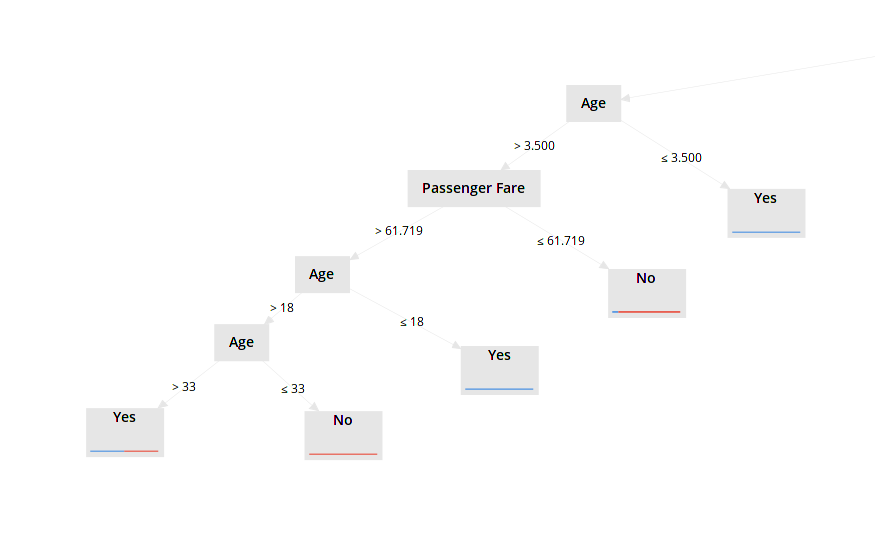
\includegraphics[width=0.75\textwidth]{02-Background/decision_tree.png}
    \caption{Decision tree for classifying survival of the Titanic}
    \label{fig:decisionTreeTitanic}
\end{figure}
One method to overcome the inherent overfitting problem in decision trees is to use a \emph{random forest} classifier. This classifier is constructed as a number of different decision trees and predicting a class based on the mode of the individual tree predictions.

\par

Another form of classifier is based on a \emph{mixture model}, where a number of probabilistic distributions are fit within the feature space. Generally speaking these are multivariate distributions as the feature-space contains more than one dimension. In most applications a Gaussian distribution is used, so this model is referred to as a Gaussian Mixture Model (GMM). The functionality of this system is based on grouping neighbouring observations in the feature-space to produce a number of Gaussian distributions, and based on the proportion of each class in each distribution, a class can be predicted from a given observation based on the distributions into which it fits.

\par
\begin{figure}[ht]
    \centering
    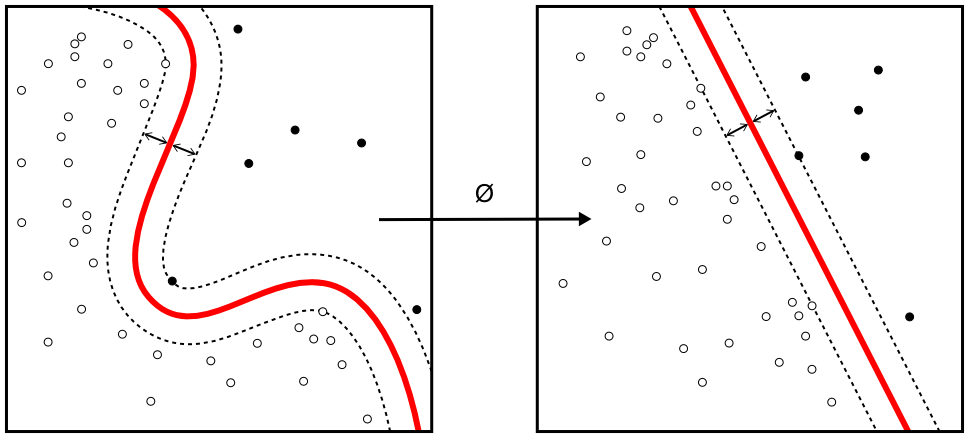
\includegraphics[width=0.75\textwidth]{02-Background/Kernel_Machine.png}
    \caption{Mapping function in a support-vector machine \cite{svmDiagWc}}
    \label{fig:svmMapping}
\end{figure}
A Support-Vector Machine (SVM) is another form of classifier that is commonly used in classification applications. The functionality of an SVM is to determine the hyper-plane that maximises the separation between the classes. A hyperplane is defined as an (N-1)-dimensional plane in an N-dimensional space, such as a line in a 2-D space, or a 2-D plane in a 3-D space. While this is quite similar in principle to logistic regression, the benefit of an SVM is through the use of the \emph{kernel trick}. In order to determine the parameters of the hyperplane, the features must be passed through a \emph{mapping function} which rearranges the features into a higher-order feature space to be separated by such a hyperplane. This mapping function is illustrated in Figure \ref{fig:svmMapping}, where an n-degree polynomial is used to map the features. For complex systems with a large number of features and a high-order mapping function, the resulting feature-space is prohibitively large. The kernel trick is a process used in this case to efficiently find a complex mapping function without explicitly requiring the mapping function to be computed. This allows for a well-performing classifier with a relatively low training complexity.

\par

Neural networks are a form of machine learning models that have recently begun to replace other methods in classification applications. One benefit of a neural network is that through training it can begin to identify and isolate its own features in the observations, allowing for more effective feature extraction in the system with less pre-processing of the data required. The model is made of a layer of input nodes, a layer of output nodes, and a number of "hidden" layers between the two. Each node in the network is a neuron-like unit, taking a number of input values, applying a non-linear \emph{activation function} on the inputs, and producing an output value which is passed to further nodes. In training, the parameters (weights) of these activation functions in each node are adjusted to fit to the training data. Training is done through the comparison of the output of the network with the intended output. The comparison is done through a loss function, which quantises the overall error in the network for the given node-weights. By taking the derivative of the loss function, a gradient can be found at each point in the weight-space for the network which determines the change in weights required for a reduction in the loss. Through iterative steps in the gradient direction for the training data (a process known as \emph{gradient descent}, the model can converge on a points of higher performance. The universal approximation theorem states that a sufficiently large neural network can approximate a continuous function arbitrarily well, which is to say that a neural net should scale well for any classification/regression problem.

\chapter{Related Work}
\label{chap:relWork}
\section*{Chapter Outline}
In this chapter we review prior studies related to the work carried out in this investigation, comparing the methods in which the work was conducted and the results found. We look at the state-of-the-art for a number of the domains and explain how we will use their findings in out investigations.


\section{Cortical Analysis}
% Discuss the work carried out by the Blue-Brain project in the extraction and analysis of the somatosensory cortex of a juvenile rat. Methodology they followed, information they amassed, topologies they discovered, and the various statistical information they collected.\\
% Short segment on the work related to LNP estimation, and how it differs to the estimation we need.
% \begin{itemize}
%     \item BBP, what they did, how they did it, and they data they supply.
%     \item Research into LNP estimation (STA STE etc)
% \end{itemize}

\begin{figure}
    \centering
    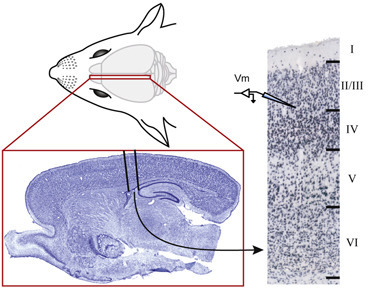
\includegraphics[width=0.65\textwidth]{03-Related_Work/ratbrain2.jpg}
    \caption{Segment of analysed brain \cite{reconSim}}
    \label{fig:ratbrain}
\end{figure}

\subsection{Source Data Extraction}
\label{chap:relwork:bbpData}
Previously mentioned was the work carried out by the Blue-Brain Project on the analysis of the somatosensory cortex of a juvenile rat, the result of which is used in this study as the source dataset for the simulated neurons \cite{reconSim}\cite{bbpTop}. This dataset comes from the reconstruction of a cortical column of the brain, where a small segment of about 0.3mm\textsuperscript{3} volume was extracted as shown in Figure \ref{fig:ratbrain}. This segment comprised of around 31,000 individual cells and about 36 million synaptic connections. The reconstruction comprised of two main parts: Reconstruction and classification of topologies; and reconstruction of the electrophysiology. For the reconstruction of topologies, 3-D reconstructions of neuronal morphologies were obtained from another study of $300\mu m$ thick brain slices \cite{markram1997physiology}. From these reconstructions, the morphologies were classified by whether they were excitatory or inhibitory, and further by the cortical layers into which they belonged. These were then correlated with the brain sample, and various methods were used to reconstruct the topologies found within the sample. As the samples consisted of brain samples, some of the topologies were truncated at the slice-edge. A number of "repair algorithms" were applied to reduce the negative effects of this truncation. These algorithms were based on first determining whether or not the topology truncation was indeed caused by the sample slice and not just the given shape of the topology. If the truncation was found to be caused by the sampling method, then a "regrowth" process was applied with a separate process depending on whether the regrowth was to a dendrite or an axon. The regrowth process takes into account the morphology of the cell, as well as the assumption of cell symmetry. While the process could not recover the exact morphology of the given sample, it was capable of recovering the cell to a "workable" state which fit the overall morphology, statistically speaking. Various corrections were also taken into account due to tissue shrinkage which may otherwise skew the reconstructed topologies.
\par
\begin{wrapfigure}{R}{0.45\textwidth}
    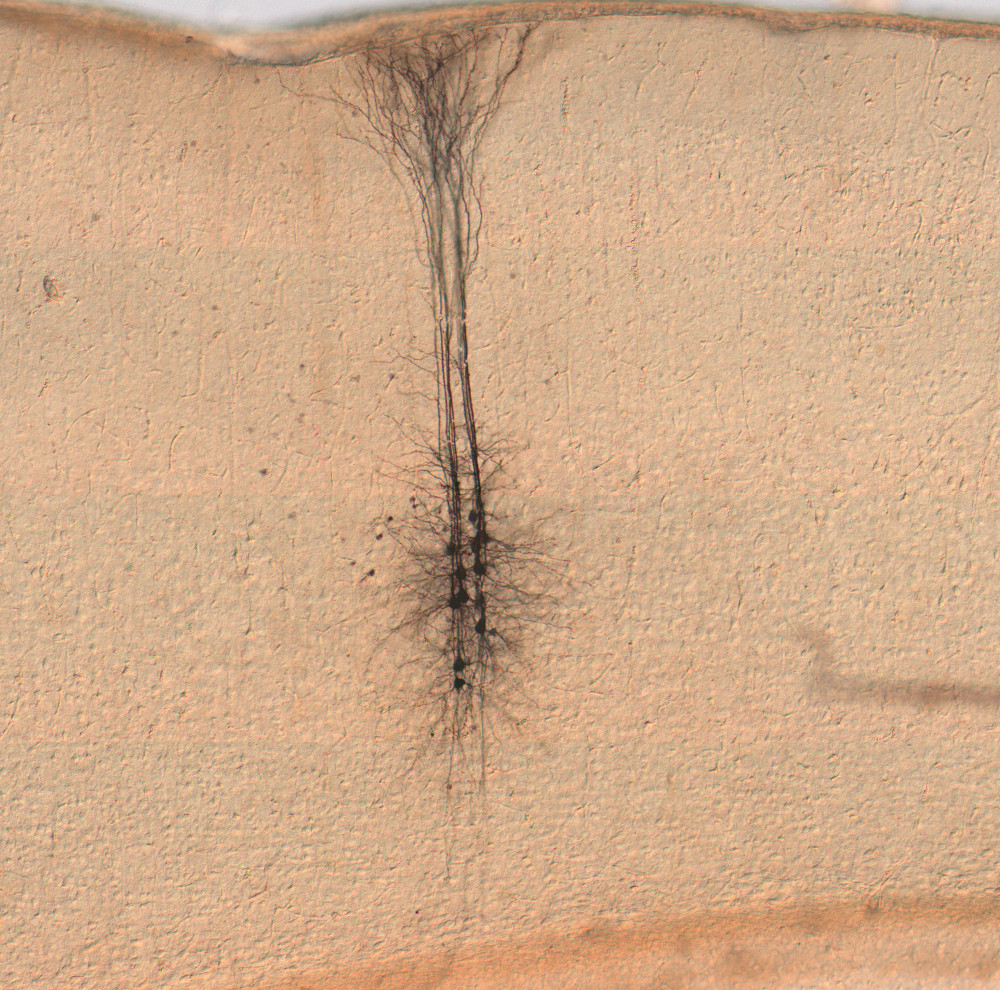
\includegraphics[width=0.45\textwidth]{03-Related_Work/l2brain.jpg}
    \caption{Sample of electrically-stimulated neurons \cite{nmcPortal}}
    \label{fig:leccyStimNeuron}
\end{wrapfigure}
To reconstruct the electrophysiology of the neurons in the brain sample, a number of in-vitro recordings were taken through the stimulus of a segment and expert-classifying the resultant waveform into one of 11 electrical types in table \ref{tab:e-type_table}. These stimulus protocols mostly dealt with the application of varying current and voltage levels over time and were all of a set of previously defined protocols: IDRest, APWaveform, and APThreshold \cite{wang2002anatomical}\cite{stimProtMark}). An image of a sample of electrically stimulated neurons is shown in Figure \ref{fig:leccyStimNeuron}.\\
Following the reconstruction of the neuron morphologies, electrophysiological properties, and overall network, analysis was done on the distribution of the various neuronal properties throughout the cortical segment. Of interest to us is the analysis of the pathways between any two neuron m-types. This was done by taking all pathways that exist between any 2 cell types (taking layer and m-type into account, disregarding e-type). For each pathway, the statistical values for parameters of the pathway anatomy, and for the path physiology were given. The parameters of the pathway anatomy largely deal with the connection in a physical sense, such as the mean/standard deviation (st.d.) of the number of synapses per connection, the mean/st.d. of the number of convergent/divergent neurons, as well as the connection probability. The parameters of the pathway physiology deal with the parameters of the pathway in a signal propagation sense, such as the mean/st.d. latency in the pathway. \\
\par
Following the reconstruction and analysis of the cortical column, the data was collected and published by the Blue Brain Project. A major contribution by the Blue Brain Project is the \emph{NMC Portal} \cite{nmcPortal}, an online portal which houses all data and publications undertaken in this research. The portal has a number of interactive "fact-sheets" which outline the analysed pathways between neurons, as well as renderings of the full reconstruction and videos of the network being simulated.\\
Through the portal it is also possible to obtain a copy of all experimental data. For each reconstructed cell (including layer, m-type, and e-type, along sub-variations) all data is supplied to replicate the neuronal simulation. This includes 3-D morphology descriptors, electrophysical mechanisms for the synapse types, as well as a list of all synapses (with parameters) available on the cell's dendrites. The cellular data files are discussed later for the simulation of the cells.\\
The portal also supplies the pathway information (physiology and anatomy) for each neuron-to-neuron pathway in JSON format. The JSON (Javascript Object Notation) format is a human-readable data format which represents a hierarchical set of key-value blocks. It can be used to specify a hierarchy of objects, each with a set of named parameters and associated values. In this format it is possible to quickly load the statistical data for analysis. A sample JSON data entry for pathway physiology can be found in \ref{ap:pathPhys}. This, again, is discussed in more detail later.

\subsection{Application of the LNP Model}
In Section \ref{chap:back:neurons} we discussed the Linear-Nonlinear-Poisson (LNP) cascade model of neuron characterisation. This model has been used experimentally in the analysis of the response of neurons in retinal ganglion cells \cite{lnpInBrain}. Here, the linear-nonlinear segments of the LNP model are joined in concept to be treated as a single block that takes an input stimulus and produces a response function which gives the output spike-rate. This response function is defined by
\begin{equation}
    \label{rsLnp}
    R(\vec{s}) = N(\vec{w} \cdot \vec{s})
\end{equation}
where $\vec{s}$ is the input stimulus, $\vec{w}$ is a vector of the same dimension of $\vec{s}$ representing the linear filter, and $N()$ is a function representing the non-linearity. The reason the linear-nonlinear segments are joined is that it becomes easier to predict $R(s)$ if this assumption is made, as this way the \emph{Spike-triggered average} (STA) metric can be used. The STA is defined as the average stimulus that leads to an output spike, and is calculated by taking a sum of the input stimulus values for each time-step that led to an output spike, divided by the total number of spikes, i.e.
\begin{equation}
    \label{staLnp}
    \vec{a} = \frac{ \sum_{t=1}^{T}\vec{s_{t}}f_{t}}{ \sum_{t=1}^{T}f_{t} }
\end{equation}
where $\vec{a}$ is the spike-triggered average, $\vec{s_{t}}$ is the input stimulus vector at time $t$, and $f_{t}$ is the output spike count at time-bin $t$. In this case, the STA is calculated over all time-steps from 0 to T, where T is the length of the recording period. It can be shown that $\vec{a} \propto \vec{w}$, and for the calculation of the nonlinearity function $N$ it is taken that $\vec{a} = \vec{w}$. A \emph{generator} signal is then defined as $\bar{g} \approx \vec{a} \cdot \vec{s_{t}}$, i.e. the "closeness" of the input stimulus to the precalculated STA. Following this, it was found that N could be calculated using the approximation
\begin{equation}
    \label{nonlinLnp}
    N(x) \approx \alpha C(\beta x + \gamma )
\end{equation}
where $\alpha$ is the maximum firing rate for the given neuron, $\beta$ is the sensitivity of the nonlinearity function to the generator function $\bar{g}$, and $\gamma$ is the "maintained drive to the cell", used to produce spikes in the absence of input stimulus. These parameters are selected to best fit the cell output based on least squared error. In testing, it was found that this method produced neuronal models with a root-mean square (RMS) difference of about 0.384 spikes per bin versus the observed actual output spike train. It was also noted that the RMS difference of averaging prior output results from the cell analysis was about 0.382 spikes per bin, indicating that the LNP-estimated model was nearly as accurate as the results from physically measuring the voltage at the cell.


\section{Neuronal-Link Parameters}
\label{chap:relWork:nrnLinkParams}
% TODO: Short section discussing the theoretical and experimental related work on analysing the mutual information of a neuronal link, and how its different to what we did.
% \begin{itemize}
%     \item Look at different papers describing the mutual information of a synaptic connection (i.e. the complex ones)
%     \item Mention the network tomography paper on delay estimation
%     \item Maybe find another bit of research on delay estimation with cross-correlation
% \end{itemize}
In Eq. \ref{eq:mutualInf} we stated the expression of the mutual information of a discrete memoryless system and stated that this was one of the models of expressing the metric, with other models fitting better to other types of systems. Prior work investigating the mutual information in a neural link has expressed the entropy of a source through the time-binning of the spike train, and defining the set of possible symbols as the possible neural response within the time period \cite{spikeTrainInfo}. For a window of length $T$ and a time-bin of length $\Delta\tau$, this leads to a symbol set of size $N = T/\Delta\tau$. Using the expression for entropy given in eq. \ref{eq:entropyDiscr}, the "naive" estimate of the neural entropy is given as
\begin{equation}
    \label{eq:naiveEntr}
    H(X)_{naive} = -\sum_{i=0}^{N}p(x_{i})\log_{2}(p(x_{i}))
\end{equation}
where X is the random variable, and $x_{i}$ is some symbol in the symbol set. The issue presented with this model is that a large data set is required to converge on a true entropy value. A possible workaround that was presented is to instead calculate a lower and upper bound on the entropy value which is robust regardless of dataset length. The lower bound presented is given by
\begin{equation}
    \label{eq:lowerEntr}
    H(X)_{lower} = -\sum_{N_{sp}}{P(N_{sp}) \times \log_{2}\left[P(N_{sp})\frac{2n_{c}(N_{sp})}{N_{obs}(N_{sp})[N_{obs}(N_{sp})-1]}\right]}
\end{equation}
where $N_{sp}$ is the "distribution of words with a fixed spike count", $n_{c}(N_{sp})$ is the "number of coincidences observed among the words with $N_{sp}$ spikes, $N_{obs}(N_{sp})$ is the "total number of occurrences of words with $N_{sp}$ spikes", and
$P(N_{sp})$ is the "fraction of words with $N_{sp}$ spikes". Similarly, an upper limit on the entropy was expressed as
\begin{equation}
    \label{eq:upperEntr}
    H(X) \leq \frac{1}{\Delta\tau}\left[H_{T+\delta\tau}(X) - H_{T}(X)( \right]
\end{equation}
for all T, where $H_{M}(X)$ is the entropy of X for some window length M. From this definition of entropy, it was found that the information rate (i.e. the mutual information) of the system increased with an increasing entropy, as expected.

%TODO:\textbf{Might add more here if there's enough time: delay estimation with cross correlation; and the fourier-transform tomography delay stuff}

\section{Classification of Neuronal Circuits}
% Discussion of Alaa's work (among others) on the classification of neurons in neuronal circuits. Also discuss topology discovery.
% \begin{itemize}
%     \item Alaa's work on cell classification
%     \item Alaa's work on topology discovery
%     \item Some more research here on other work in this area
% \end{itemize}



Prior work has investigated the classification of network parameters given simulated endpoint data \cite{ekkyProj}. A layer 5 cell was selected (layer 5, DBC m-type, cAC e-type), and 4 different combinations of 4 pre-synaptic cell m-types were selected: \{\{PC,PC,LBC,IPC\}, \{MC, SP, STPC, BP\}, \{PC, NBC, UTPC, UTPC\}, and \{PC, PC, STPC, IPC\}\}. The post-synaptic cell was then stimulated, and the soma-membrane voltage was measured for each of the pre-synaptic groups. The features used in this classification model were the frequency, delay, and number of spikes, along with the voltage-vs-time measurement of soma-membrane potential, and the average power spectral density. The overall accuracy of this classification model was about 83\%, with the model performing well for all pre-synaptic groups other than \{PC,PC,LBC,IPC\}.
\par
As well as cell-group classification, a topology-discovery classifier was also investigated. The intention of this classifier is to estimate the type of topology from which the measurements were taken, based on a small set of topology-type classes. In this case, the topology classes selected were {4-leaf star, 2-leaf star, and individual}. Here, "individual" means a single cell, while the star topologies are based on a network with a single central node, and a number of connected leaf nodes surrounding the centre (this is discussed in more detail later). The topologies investigated were relatively small and the classifier achieved accuracies as high as 99.37\% when classifying the 2-leaf and 4-leaf topologies through the use of decision trees. \\
While the research conducted focused mainly on a relatively small number of neurons, we expand on this by investigating similar types of classification with more complex sets of classes, such as with the full set of cell-possibilities.\\

%TODO:\textbf{Might add more here if there's enough time: theres been other research into cell-type classification that would fit well here.}

% As well as this, we hope to infer more link-level characteristics of the network rather than only
% classification of the circuit type, which could be done through the use of theory from network
% tomography.

% \par
% Network tomography deals with the inference of network characteristics such as link-by-link
% loss rates and delay distributions from a finite number of endpoint measurements [7]. It is
% achieved by treating the problem as a linear model, y = Aθ +  with known routing tables (A,
% a matrix) and measured endpoint data (y, a vector), solving for a vector of packet parameters
% (θ). The final term, , represents the noise term of the system (such as perturbations in the
% packet parameters). In many network systems, the size of the matrix tends to be quite large,
% and so solving for the packet parameters is non-trivial. As it is a linear problem, inversion
% is used which has well-documented solutions for possible approaches to solving the problem.
% In general this comes down to either solving for a linear combination of the parameters, or
% solving through the use of regularisation to bring identifiability. In this project we will apply
% the theory of network tomography to some common cortical circuit topologies in order to infer
% these link-level characteristics.

% \par 

% The circuit topologies that will be later investigated are based on the findings of [5] which
% investigated the structure of the networks found in the reconstructed juvenile rat somatosensory
% neocortex. Despite this reconstruction being comprised of roughly 31,000 cells, it was found that
% the average separation of any two cells was 2.5 synapses, indicating a small-work topology. This
% indicates a large degree of inter-layer connectivity, which is a point that will be investigated
% in our research during the construction of the various circuits. The article notes that the
% large-scale network properties analysed were likely the result of the constraints of the cortical
% reconstruction itself (such as the limitations of the cortical slices reducing the extent to which
% the axons were captured). This, however, should not be a major issue in our research as we will
% be dealing with circuits at a scale far below that of the full reconstruction and so the findings
% of the article dealing with smaller-scale network properties will be applicable.
\chapter{Methodology}
\label{chap:meth}
\section*{Chapter Outline}
In this chapter we describe the steps taken to carry out the experiments conducted in the various experiments. We describe the tools and frameworks used to generate and process the data, and explain how these tools were used to create our own experimentation framework for the rapid simulation of a large number of uniquely generated networks.


\section{NEURON tool}
%Description the NEURON tool, how it works, and how we use it.
The NEURON tool is a simulation framework developed by researchers at Yale University for the \emph{in-silico} analysis of individual and networked neurons, and originally released in the 1990s. The framework provides a number of tools for the construction, simulation, and recording of individual cell-models from biological principle building-blocks as well as networks built from individual neuronal models. The main goal of the framework is to simulate the mathematical models that describe nerve cells, and the tools provided are intended to allow for easier interfacing with the model simulations. Use of this approach has a number of benefits over other simulation methods \cite{neuronSimEnv}. One such benefit is that the framework allows for the expression of the problem space in biological terms, without any need for the user to explicitly convert from the neuroscience-context into computational analogues. Another benefit is the supporting tools included with NEURON that allow for manipulation of the simulation environment (timesteps, type of simulation model etc.) as well as the inclusion of tools for easily collecting, converting, and graphing the measurements around the simulation space. On top of the graphing tools, the framework includes a full set of GUI-creation tools with a number of predefined "widgets", allowing for the rapid design and implementation of simulation GUIs that allow for graphical control of the simulations. Finally, the NEURON tool has had considerable work done on improving the efficiency of its backing computational engine, using "special methods that take advantage of the structure of nerve equations". The framework also has support for multi-threading which can take advantage of modern multicore processors for even more efficient computation.

\par

There are two main methods of interfacing and controlling the NEURON framework: through the High-Order Calculator (HOC) language, and through Python.\\
The HOC language was originally designed as a floating-point calculator featuring C-like syntax (and indeed was co-developed by one of the original developers of the C programming language) \cite{kernighan1979unix}. Since its introduction in 1984, the language has been extended beyond simple calculator-syntax into a more general-purpose programming language, such as through the introduction of object-oriented syntax. Its calculating background, however, makes it a suitable choice for the control of the NEURON tool due to the close relation between the neuronal cells and the mathematical models through which they are simulated.\\ %A sample section of HOC code used in the creation of these neuronal simulations is shown in listing \ref{lst:hocSample}.\\
Python support was more recently added to the NEURON framework, allowing for much the same interfacing capabilities as with HOC. As well as interfacing directly with the framework, it is also possible to interface the Python segments with HOC source files, allowing for hybrid programs to be run. The majority of the simulation code used in the course of this investigation was written in Python, with a small number of HOC-source interfaces. This allowed for the use of the large repository of Python libraries which greatly aided with the creation of the simulations and the conversion between data types. A more detailed of the specific work undertaken in interfacing with NEURON is discussed later.

\par

The basic building block of a neuronal model in NEURON is a \emph{section}. A section can be thought of as a length of cable with a specified geometry given by length and diameter. The electrical characteristic of the section is specified by the \emph{axial resistivity}, expressed in ohm-cm. Sections can be interconnected, branched, and joined to form the overall structure of the neuron. The connectivity of the sections is hierarchical in nature, in that each section has a parent section (and thus may have numerous child-sections). Each section is subdivided into a specified number of \emph{segments}. This is done for simualtion purposes, as the membrane potential is calculated at the ends of each segment within the section. As the number of segments in a given section is specifiable, the user has granular control over the complexity of the computation for each section. By defining the geometry and electrical characteristics of a neuron in term of a hierarchy of interconnecting sections, it is possible to quickly generate a computational model of the cell in the NEURON environment.
\\
Synapse models can be created in NEURON in a number of different ways. The simplest method of creating a synapse is to use one of the predefined synapse models, such as the \emph{ExpSyn} object, a construct built-in to the framework that defines a synapse with a discontinuous change in conductance at an event (i.e. a voltage spike) followed by an exponential decay. This models the concept of a release of neurotransmitters generating a resultant current in the post-synaptic dendrite, a process described previously in \ref{chap:back:neurons}. The ExpSyn object has a number of parameters that can be specified: the decay time constant ($\tau$) in ms, the reverse potential (e) in mV, and the synaptic current (i) in nA. Another more complex method of modelling synapses is to define a NEURON \emph{mechanism}, which is a mathematical description of the functionality of some process. This is quite a flexible approach as there is a greater level of control over the functionality of the process, and it is therefore possible to model specific biologic synapse forms, such as the NMDA synapse discussed in \ref{chap:back:neurons}. 
The synapse is "connected" to a section on a cell, in much the same way that sections connect to each other. At this point, a change in the membrane potential of the synapse will result in a corresponding change in the membrane potential of the section directly connected to the synapse, which can then propagate through the section and further through the entire neuronal model.
One important consideration with the form of the synapses in NEURON is that rather than respond to a potential as they would in practice, the simulated synapses instead respond to an \emph{event}. An event is a type of construct in NEURON that represents exactly that: an event. It defines a point in time in the simulation during which "something" has happened, without explicitly specifying what the "something" is. In the case of the synaptic models, the event is generally generated when the membrane potential crosses a certain threshold, indicating a voltage spike. The synapse object receives the event (without any information of the actual voltage that generated it) to which it can respond with its own event, or more commonly by adjusting its membrane potential. An event can also have a weight associated with it, which can be used to specify the intensity of the event.
\\
Another feature required for most simuations is one or more stimuli. In NEURON, a given stimulus is usually implemented in three parts: a \emph{NetStim} object, a \emph{NetCon} object, and a synapse. The NetStim object generates a spike train, similar to the type of output spike train that one might expect as the response of a neuron. This is intended to emulate some system of pre-synaptic neurons which generate a set of spikes which are delivered to the neuronal model that is to be simulated in the framework environment. The NetStim object is a built-in feature to the NEURON framework, and has the following parameters:
\begin{itemize}
    \item NetStim.interval - mean time between spikes in ms
    \item NetStim.number - average number of spikes generated
    \item NetStim.start - the desired time offset from start of simulation to generate the first spike, in ms
    \item NetStim.noise - proportion of additive noise to include, in a range of 0 to 1.
\end{itemize}
As the simulation runs, the NetStim object will generate a number of \emph{events} representing voltage spikes. These events must be delivered to a synapse of the cell being simulated in order for the cell to respond. The two objects cannot be connected in the same way as the model \emph{sections} can, as they are dealing with events rather than electrical currents. Instead, the connection is typically implemented using a \emph{NetCon} object. The NetCon object has multiple purposes, however in this case it is used to connect an event-generator (in this case a NetStim object) to an event-receiver (a synapse). No other parameter is required by the NetCon object in this use case, as it is simply delivering an event, however it is possible to also specify an event-delivery delay in ms, and an event weight.\\

Connecting 2 neuronal models together (such as in the case of the simulation of a network) is similar in principle to the creation of emulated stimuli, however instead of using a NetStim object to generate spike-events, instead a simulated neuron generates a certain output voltage over time which must be used to generate the events. This is done using a NetCon object again, however in this case it is used in a slightly different way. Previously, the NetCon object was used to simply take an event-generator and deliver the events to an event receiver; in this case, the NetCon object takes a voltage generator (i.e. the output of a neuron), and uses a pre-defined threshold on the voltage to generate a new event, which is then delivered to an event receiver. In this case, the "source" end of the NetCon is connected to the axon membrane of the pre-synaptic cell. A threshold voltage can then be specified, which represents the voltage level that the membrane must cross for an event to be generated. A delay and weight value can also be specified, as above. The output side of the NetCon can then be connected to the synapse on the dendrite of the post-synaptic cell. With this, the 2 neurons are connected and a network is formed. Artificial stimuli (such as with a NetStim) connected to the pre-synaptic cell with stimulate it, causing the neuron to generate an output voltage spike-train. This spike train is then thresholded by the NetCon object, generating events which are delivered to the synapse at the dendrite of the post-synaptic cell where the release of neurotransmitters is simulated, raising the potential of the section. This is the functionality of the neuronal simulation which were used in this study. In practice, multiple stimuli are used, and multiple NetCon->synapse connections are used between cells in the network with varying delay, threshold, and weight parameters.\\

With the network of neurons created and under simulation, it is necessary to also measure the voltage at various points amongst the neurons. This measurement is implemented using a NEURON \emph{Vector}, another built-in object in the framework. The Vector object is similar to the C++ std::vector class, representing a dynamic array that can be added to during runtime. In the NEURON framework, the Vector object represents a list of floating-point values and can be programatically added to and read from. An addition function of the Vector object comes from the use of its member function \emph{Vector.record()}. This function allows the user to specify a section voltage-reference (a member of each NEURON section representing the membrane potential of the given section), and it will then record the section voltage during simulation. The user has additional parameters to specify either the recording time-step (the discrete steps in time at which the voltage will be sampled), or even a predefined vector of time-points to sample at. Following simulation, the Vector object will contain the recordings of the section which can be easily converted to Python-native lists for manipulation, or saved to disk (or indeed both).\\

\subsection{Cell-data Source}
%Blue-brain project and the model files they provide. What the files contain, and how they're used in NEURON
In \ref{chap:relwork:bbpData} we discussed the data collected and supplied by the Blue Brain Project (BBP). This data is supplied in a format that is compatible with the NEURON framework, including sample HOC files for initiating and simulating single-cell networks. Each cell supplied is categorised by the layer, m-type, e-type, and variation (multiple variants may exist for the same layer;m-type;e-type group). For example, the cell titled "L1\_DAC\_bNAC219\_1" represents a layer 1 cell of DAC m-type and bNAC e-type. For each cell, a number of data-files are supplied. One of the main files is the morphology descriptor. This file contains the complete description of the entire morphology of the cell, formatted as the NEURON-compatible section-segment hierarchy. Rather than manually specifying each section in HOC code, the morphology descriptor can be loaded in about 3 lines of code using the \emph{Import3d\_Neurolucida3()} and \emph{Import3d\_GUI()} functions. These functions read the section descriptor file, and construct the entire cell morphology in the environment. The morphology is also pre-segregated by cell-portion (soma, dendrites, axon etc.) and each can be explicitly accessed. The supplied data also includes a programatic of the cell's biophysical properties. These properties represent the specific electrical characteristics of various sections within the neuron and are vital to accurate simulation of the cell. The characteristics are defined by NEURON mechanisms, discussed previously, which represent the response of an object to some stimulation in a mathematical sense. A description of the cell's synapses are also included. This includes the location, synapse type, and synapse parameters for each synapse in the dendritic branches of the cell, which are again easily loaded programatically. \\
\begin{figure}[ht]
    \centering
    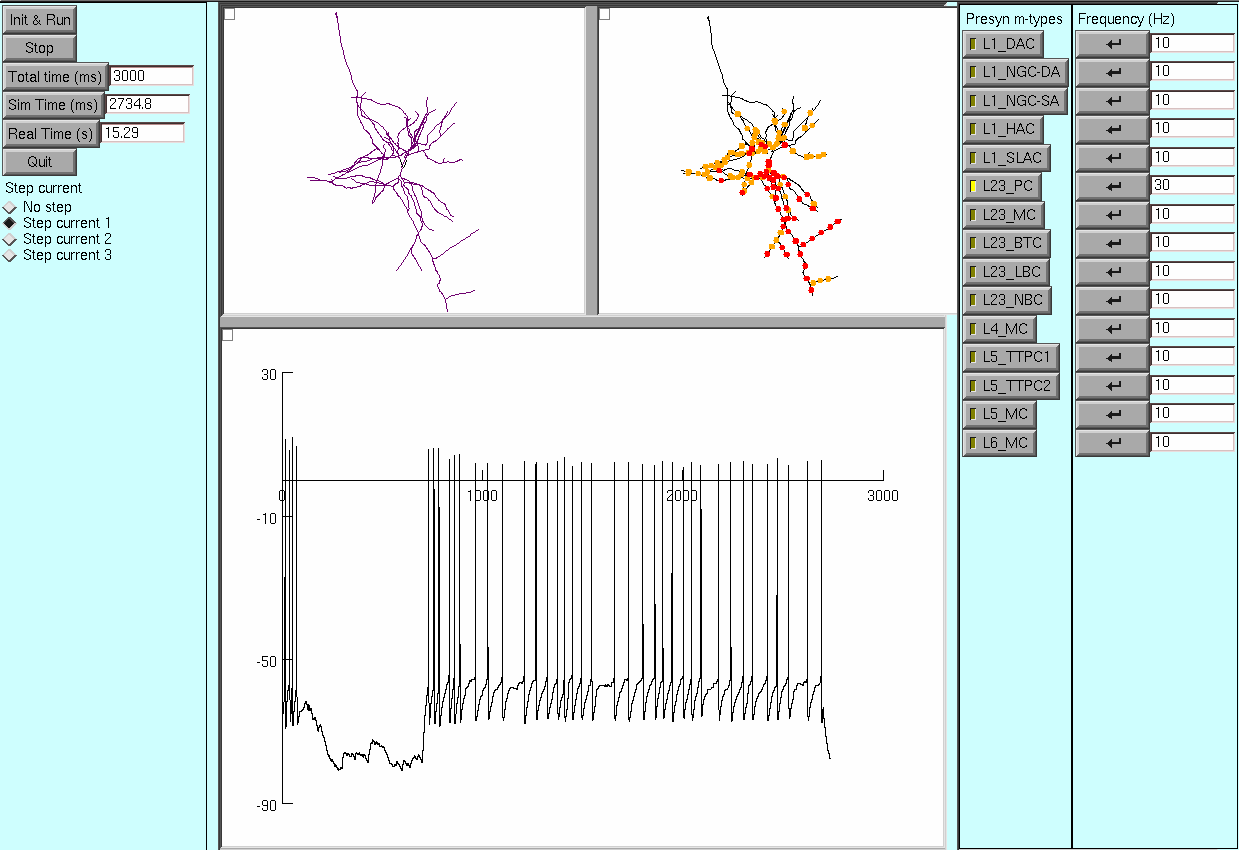
\includegraphics[width=0.8\textwidth]{04-Methodology/nrnSample.png}
    \caption{NEURON simulation GUI generated by BBP data files}
    \label{fig:bbpNrnGui}
\end{figure}

Along with the various cell descriptors, sample HOC files are also included which instantiate a NEURON session, load all of the cell data into the session, sets up a number of pre-synaptic stimuli (using the NetStim approach discussed above) and then constructs a GUI interface for interactively controlling the simulation. The result of running this sample HOC instantiation file is shown in Figure \ref{fig:bbpNrnGui}. The left-hand panel of the generated GUI are used to control the simulation, allowing the user to start and stop the simulation along with specifying the length of the simulation to run. The centre-top panels show the loaded cell's morphology and areas on the cell to which synapses are connected and stimulated. The lower panel shows the graph of the membrane voltage over time (updated in real-time as the simulation runs), which clearly shows the spike-train output of this neuron. The right-hand panel is used to enable/disable the various pre-synaptic emulated cells (using NetStim objects) that can be connected to the neuron in the simulation. The frequency of the spikes (i.e. the interval property of the NetStim object) can also be specified to select the stimulus intensity.



\subsection{Python Backend and Support Library}
%Description of the NEURON Python API and how we used it to create the Neurpy library for quickly analysing cortical circuits.\\
%Layout of the software, output formats etc.

While the sample files given by the BBP are extremely useful and informative, they are limited in that it is not inherently easy to connect multiple cells together to form a multi-cellular network. As well as this, the use of the GUI is not a scalable approach when generating a large set of training data. For this reason, we developed a Python library to address these issues \cite{neurpyGit}.\\
The library, referred to as \emph{Neurpy} uses the NEURON-Python API to more easily construct simulations of any network form, while also allowing for either GUI interfacing (for interactive/debug purposes) as well as a more lightweight "headless" interface where the simulations are run entirely though the Python code without any need for user interaction. This headless approach also allows us to easily run multiple simulations in parallel, taking advantage of modern multi-core CPUs to accelerate the generation of test data.\\
Neurpy makes use of the data supplied by the BBP to construct the simulations. For simulation, a Neurpy "Environment" object, \emph{NeurpyEnviron}, is set up, which represents a NEURON session including all cells in the environment space, stimuli, recording vectors etc. and exists for the duration of the simulation. The \emph{pyCell} class was defined to represent a single BBP-supplied cell. The class loads in all relevant data from the cell dataset, such as the morphology, biophysics, and synapses, and allows for easy manipulation of the cell as a single, addressable unit in the environment. The cell can be translated to different points in space, however the main benefit of this class is the hierarchical structure of interconnected cells. By calling the \emph{pyCell.addChild()} function and passing another cell as a parameter, the Neurpy library will automatically connect the parent cell to the child cell using a number of NetCon->Synapse connections as described previously. Through the parameters to this function, the number of synaptic connections, as well as the delay and weight for the connections can be specified.\\
The Neurpy library also allows for easier creation of network stimuli and membrane potential measurements (referred to as \emph{probes}). Network stimuli are provided by the \emph{CellStim} class. This class represents a NetStim->NetCon pair and can be connected to one or more synapses on a given pyCell object. Another feature of the CellStim class is the probabilistic amplitude-keying option. By supplying a "symbol probability" the CellStim object will automatically enable and disable itself as the simulation run. This is to simulate the transmission of "symbols" as defined for the information theory equations in Section \ref{chap:back:infTheory}. The object keeps a list of the toggle-states it was in throughout the simulation which can later be used in processing to estimate the mutual information of the synaptic link (discussed in more detail later). The network probes (membrane measurements) were not implemented in a specific class as the creation of the probes is quite simple, requiring only the creation of a Vector object, and the linking of that Vector to a cell section. The Neurpy library does this and connects the Vector to the soma of a specified cell, adding the Vector object to a global list.\\
At this point the network is created as the individual cells are loaded and interconnected, the stimuli have been generated and connected to the cell models, and probes have been set up to record the network as the simulation runs. At this point, there are two options available to the user: create a GUI window for interactive simulation, or run a headless simulation. In the first case, a GUI of the same structure as Figure \ref{fig:bbpNrnGui} is created with all loaded neurons visible in the centre-top panels. The user can then set simulation parameters and run the simulation, observing the recorded voltage in the graph panel. This does not produce any simulation data that is saved to disk, and so was generally only used for debugging purposes. The second case (headless simulation) is done through calling the \emph{NeuronEnviron.runSimulation()} function on the Neurpy environment object, passing the filepath of the desired output data. The Neurpy library then calls on the NEURON framework to begin simulating the objects in the current session. After the simulation has completed, the library collects all the Vector recordings that had been specified, converts them to a native Python format, concatenates all the voltage data-points and exporting as a comma-separated value (CSV) file, saved to the specified data path. This entire process can be seen in listing \ref{lst:sampleNrpyCode}. In this code snippet, the Neurpy library is first imported, and an environment session is started by calling \emph{NeuronEnviron}. The environment requires the location of the BBP model and mechanism data as parameters, such that the relevant data can be loaded when creating cells. Next, 2 different cells are created: \emph{cellA} is from layer 6, with m-type BP and e-type bAC, while \emph{cellB} is from layer 1 with m-type DAC and e-type bNAC. Following this, \emph{cellB} is translated in space by 100 $\mu m$ in the y-direction. We then add \emph{cellB} as a child of \emph{cellA}, specifying that the synapse should be excitatory ("true" for excitatory, "false" for inhibitory), and that 6 synapses with weight 1.0 and delay 1.0ms should be used to connect the two cells. At this point, the 2-cell network has been created, so we can either generate the GUI for interactive simulation (as in the first branch of the if-statement) or we can run a headless simulation, passing a local filepath as our desired output file. At the end of the simulation, all output measurements will be saved to "simData.csv" and the script will exit, destroying the Neurpy (and thus NEURON) environment and freeing up memory before exiting.\\ 



While this method of hard-coding networks in Neurpy is viable and certainly easier than with the given HOC source files in the supplied BBP data, it is not ideal for the automatic simulation of large sets of networks which is required by this investigation. For this reason, a network-descriptor feature was added to the Neurpy library whereby the NeuronEnviron object can load in a description of a simulation network (including all cells, cell-to-cell connections, stimuli, and probes), which it can then automatically construct in the given session and simulate. This allows for easier scripting of the experimental process, allowing for the generation of large sets of data.



\subsection{Network Descriptor}
For the specification of networks, an XML-based descriptor was defined, similar in concept to the \emph{GraphML} format for describing network graphs. XML (eXtensible Markup Language) is a type of markup language which, similar to JSON, allows for the hierarchical description of a set of parent-child relations, specifying key-value parameters for each entry. The base block of an XML document is an \emph{element} which is a named block with a set of key-value parameters, as well as 0 or more sub-elements. There is no inherent constraint on the naming of the elements or the parameters, as the functionality is based entirely on the interpretation of the document. A simple example of an XML document is shown in listing \ref{lst:sampleXml}. The first line in this listing is the document's metadata, and contains information about the format of the rest of the document. After this, an element of type "node" is created with an ID parameter of 0, and another parameter of value 120. The node element also has 2 children, one is another element of type "node", and the other is an element of type "testData". Neither of these elements have further child elements, and so can be terminated using the "/>" terminator. The termination of the parent element can be expressed using "</node>" after all of its children have been specified.
\begin{lstlisting}[language=XML,label=lst:sampleXml]
<?xml version="1.0" encoding="UTF-8"?>
<node id="0" some_param="120">
    <node id="0_0" another_param="1" />
    <testData/>
</node>
\end{lstlisting}
As the naming of the XML elements and parameters is entirely implementation dependent, we can therefore define our own XML-based descriptor to describe the networks that we will be simulating:
\begin{enumerate}
    \item The base element of the hierarchy is an element of type "Neurtwork". All network elements will be some child/grandchild etc. of this base element.
    \item Individual cells are specified by an element of type "cell" with parameters:
    \begin{itemize}
        \item cellType - a string representing the corresponding cell in the BBP dataset
        \item id - a session-unique ID for the cell in the environment
        \item label - an optional label string for the cell
    \end{itemize}
    \item All individual "cell" elements are direct children of a single "cells" element
    
    \item Cell-to-cell connections are specified by an element of type "edge" with parameters:
    \begin{itemize}
        \item id - a session-unique ID for the edge in the environment
        \item source - the ID of the source cell
        \item target - the ID of the target cell
        \item connCount - the number of synaptic connections in the edge
        \item connType - the synapse type: 1 for inhibitory, 0 for excitatory
        \item delay - the delay in ms of the edge
        \item weight - the weight of the edge
        \item label - an optional label string for the edge
    \end{itemize}
    \item All individual "edge" elements are direct children of a single "edges" element
    
    \item Stimuli are specified by an element of type "stim" with parameters:
    \begin{itemize}
        \item id - a session-unique ID for the stimulus in the environment
        \item target - the ID of the target cell
        \item delay - the delay in ms of the stimulus connection
        \item prob - the symbol-probability of the stimulus
        \item label - an optional label string for the stimulus
    \end{itemize}
    \item All individual "stim" elements are direct children of a single "stimuli" element
    
    \item Measurement probes are specified by an element of type "probe" with parameters:
    \begin{itemize}
        \item id - a session-unique ID for the probe in the environment
        \item target - the ID of the target cell
        \item tag - an optional label string for the probe
    \end{itemize}
    \item All individual "probe" elements are direct children of a single "probes" element
\end{enumerate}

An example of a network specified with the above format is shown in listing \ref{lst:sampleNetXML}. This network consists of 2 cells, a layer 1 DAC m-type and bNAC e-type cell and a layer 1 NGC-SA m-type and cNAC e-type cell. The first cell connects to the second through 5 excitatory synapses with a delay of 5ms and a weight of 2. A single stimulus is connected to the first cell, with unspecified probability (disables the symbol-probability keying). Finally, 2 probes are specified, one for each of the cells. The tags specified in the network are used as column-headers in the output data file for easily distinguishing between the membrane voltages of the two cells.


An extension was made to the Neurpy library to accommodate the XML-based network descriptors. This extension was defined in a class called \emph{Neurtwork} which takes a path to an XML network descriptor file, reads and decodes the various elements in the document, and constructs the network in a given Neurpy session. The network loading is done entirely automatically from the XML description, and requires no further user input. Prior to simulation, however, the user may modify the session, such as through the translation of some cells (which can be addressed by their XML-defined ID parameter).\\
The benefit to this approach is that the running of the simulation can become more automated. For example, given a folder of individual network description XMLs, the code in listing \ref{lst:sampleNetRun} can be used to run through an arbitrary number of simulations (limited only by the number of network descriptors), constructing the network, running the simulation, and saving the output measurements to a separate folder. As well as this, the number of network descriptors could easily be subdivided and allocated to be run on separate CPU cores, which again allows for a speed-up in simulation time.
\begin{lstlisting}[language=Python,label=lst:sampleNetRun]
import neurpy, os
validFiles = os.listdir( "./networks" )
for idx, netXml in enumerate( validFiles ):
    neurEnv = neurpy.NeuronEnviron( './modelBase',
                                    './modelBase/globalMech' )
    neurEnv.loadTopology( netXml )
    neurEnv.simulate( "./output/v_data%i.csv" % idx )
\end{lstlisting}


% With the network represented in NEURON, a number of simulations were run. The soma membrane potential was measured for each of the cells, and a plot with the L1 and L6 measurements is shown in figure \ref{fig:sm_l1-6}. This figure illustrates the effect of signal propagation with multiple paths to end-nodes, where a single spike in the L1 cell often results in 2 spikes in L6 as the impulse from L1 arriving at L6 twice, with a delay between the arrivals due to different propagation times along the respective paths. One factor that can be attributed to the difference between the observed spike trains of the L1 and L6 cells is the biophysical properties of the cell itself\cite{markram2015reconstruction}, as well as the properties of the link between the neurons.\\
% With the reference network above completed, work was started on creating a Python framework which will support simplified construction and simulation of various network topologies in a consistent and scriptable manner. Using Python as the frontend language has a number of benefits over the HOC language used for the first example, namely that there is much better support for third-party libraries which may be helpful in future for handling intricacies such as complex network tracking.\\
% The basis for this Python framework is the creation of a library dubbed \emph{Neurpy}\cite{Neurpy}. This library serves as an interface between a Python script and the NEURON backend, dealing with the boilerplate code of any program using NEURON, such as context creation, cell morphology/mechanism loading, network construction, GUI creation, and running the simulation/collecting measured data. In this way, the frontend script for the creation and simulation of a simple 2-cell network takes the current form:
% \begin{lstlisting}[language=Python]
% import neurpy
% neurEn = neurpy.NeuronEnviron( './modelBase',   # Base directory of cell data
%                               './modelBase/globalMech' ) # Mechanism directory
% cellA = neurEn.createCell( 'L6_BP_bAC217_1',    # Name of cell directory
%                           'bAC217_L6_BP_b41e8e0c23' ) # Name of cell
% cellB = neurEn.createCell( 'L1_DAC_bNA219_1', 
%                           'bNAC219_L1_DAC_ec2fc5f0de' )
% cellB.translate( [ 0.0, 100.0, 0.0 ] )
% cellA.addChild( cellB, 0.6 )    # Connect cellA to cellB
% if genGui:
%     neurEn.generateGUI().createMainWindow()
% else:
%     somaMeasurements = neurEn.simulate()
% \end{lstlisting}
% As can be seen, the library supports both creating a GUI instance (for displaying real-time information and visualising the network structure) as well as running the network simulation without any visual frontend (for scripting and generating banks of test data).

\section{Network Generation}

While the ability to load in XML-based network descriptors makes it easier to construct session-by-session networks to be simulated, it still requires the networks to be hand-written. Thankfully, the statistical data provided by the BBP can be used to automatically generate unique networks that fit within their supplied distributions, exporting the network in the predefined XML format that can be loaded and simulated in Neurpy. As discussed in \ref{chap:relwork:bbpData}, the BBP provided a number of useful metrics on the pathway data between connecting cells. Using this data, a network generator script named \emph{NeurGen} was constructed in Python. \\
NeurGen functions by loading the JSON-formatted statistical data on the physiology and anatomy of each cellular pathway, building an internal database of statistical distributions for each of the connective parameters, and then generating a semi-random network that is unique in layout, yet still fits to the given distributions. In other words, if one were to generate a large number of these "random" networks and then recalculate the distributions for the same connective parameters, the end results should be close to the distributions given by the BBP. This means that the generator will create anatomically correct networks that would be expected to be found within the neocortex.\\
One method of creating networks using NeurGen is through the \emph{createRandomNetwork()} function. By passing the number of cells that should be in the network to the function, it will create and return the randomly generated network. The generated network has no complex/branching connections, it is a serial line of neurons with a single path from the head cell to the tail cell. The network is generated iteratively; the first cell is selected at random from the set of all possible cells. With the head cell selected, it is temporarily named the pre-synaptic cell. The generator then finds all pathways from the statistical data that has this cell as a pre-synaptic type. With the list of possibly pathways found, a probabilistic score is assigned and the network selects the pathway from the set based on the "connection probability" parameter in the pathway anatomy. With the pathway selected, so too is the post-synaptic cell. Other pathway parameters can then be taken (such as the distribution of synapse-count per connection, edge delay, etc.) and the Python function \emph{normal()} is used to sample the distribution. The \emph{normal()} function takes a given value for the mean and standard deviation of a distribution, and samples it. With the connection between the two cells set up, the generator can now temporarily treat the post-synaptic cell as the new pre-synaptic cell, and repeat the process. This is repeated until the required number of cells have been found.\\
With the cells selected, the generator then assigns a stimulus to the head cell. As well as this, probes are assigned to each of the network's cells. At this point, the network is fully defined and it can be returned to the caller where it can then be written to the disk as an XML-formatted file. Using this network generator, we can generate a large amount of sample networks in a very short amount of time and with minimal effort. A snippet of code using the network generator to create 10,000 unique networks with between 5 and 20 cells per network is shown in listing \ref{lst:netGenSamp}.
With the networks generated, the directory containing the descriptors can then be used in the form of the code snippet in listing \ref{lst:sampleNetRun} to simulate all networks automatically.

\subsection{Template to Topology Generation}
The generation of random networks can be useful in some circumstances, however for this investigation we deal with specific network topologies that cannot be constructed through the \emph{createRandomNetwork()} function described above. For this reason, the NeurGen tool was extended to accept as input a topology template. The template takes a form quite similar to the XML-network descriptor used by Neurpy, however the major difference is that it keeps only the overall network shape (number of cells, which cells connect where, the stimuli, and the probes) without requiring any specific data to be specified about any of the network components. Cell types requirements can be specified using a regular expression (a method used for matching against strings) where the user may specify an expression that a cell must match in order to be selected for that node. In this way, the network shape can be maintained, while the cell-types that slot into the topology can be randomly selected from a user-constrained set. An example network template for a 4-leaf star topology is shown in listing \ref{lst:4leafTop}. Here we can see that the central node of the star may only be a layer 1, m-type DAC, e-type bNAC cell. Meanwhile, "Node1" of the network must be from layer 2, with no constraint on m-type or e-type. The final 3 star nodes are not constrained at all and can be any cell, provided the pathway data exists for it.\\
By running the NeurGen \emph{createNetwork()} function and passing the filepath of this topology template, the generator will again create a network that fits both to the statistical distributions given by the BBP as well as to whatever cell-matching constraints listed in the template file. In this way, an arbitrary number of unique networks of a specific topology may be generated and simulated, offering a wide variety of simulation data for analysis.

\section{Simulation Framework}
\begin{figure}[ht]
    \centering
    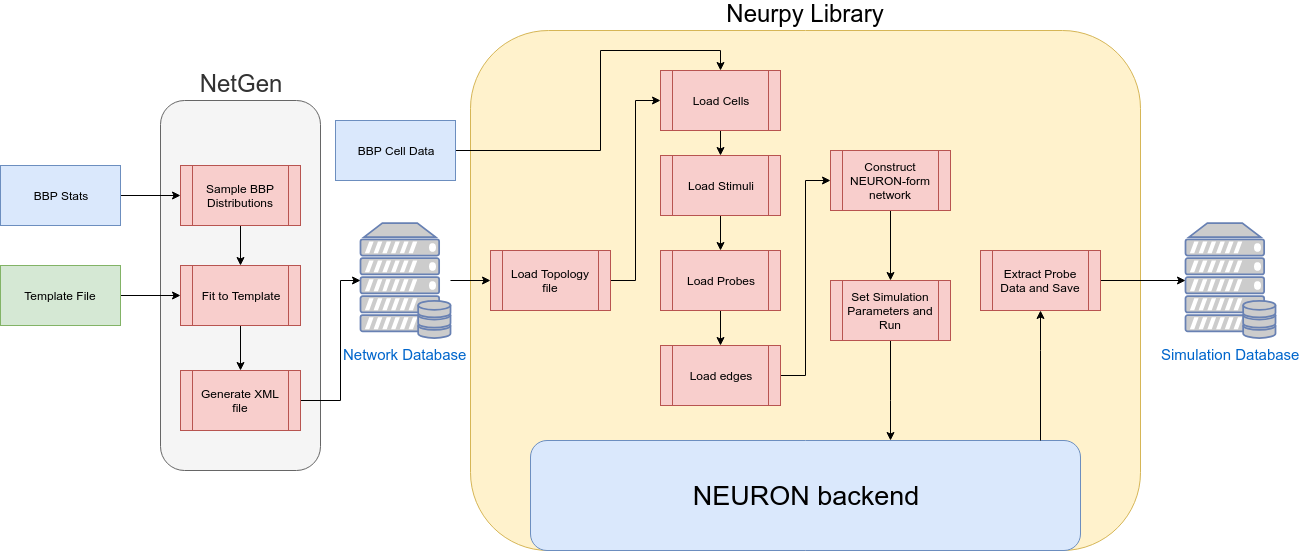
\includegraphics[width=\textwidth]{04-Methodology/SimFW.png}
    \caption{Structure of experimental environment}
    \label{fig:nrpySimFw}
\end{figure}
At this point, all the components of the simulation framework have been defined. An overview of the entire process is shown in Figure \ref{fig:nrpySimFw}. The general flow of this process is from left to right. On the left we begin with the network generator. We feed the statistical data on the cell-to-cell pathways from the BBP along with a topology template into NeurGen. Within NeurGen we can then generate a large number of unique individual networks, which we store as the "Network Database". After the database of networks has been created, we can begin feeding this into the Neurpy library, file by file. For each network file, Neurpy loads the specified cell model data from the BBP, loads and connects the required stimuli, loads and connects the required measuring probes, and finally connects the cells together to form the in-session network. Following this, the session simulation parameters are set (timestep, simulation length etc.) and Neurpy instructs the NEURON backend to begin the simulation. After the simulation has completed, all data is extracted from the probe vectors, converted and concatenated in a Python-native format, before being written to the disk. By repeating this for all network files, we create the "Simulation Database" which contains the voltage-vs-time data for each probe in each simulation, which we can then use for analysis.\\
A complete listing of the code used to run the simulations from the network files is shown in Listing \ref{ap:simCode}. This is the code that was run over the course of several days to simulate over 100,000 individual networks, and so it was made to use multiple cores to accelerate the simulations. When running, each process reports its current network ID (an index within the list of overall networks), as well as its current timestep in the simulation. The code also calculates the average number of simulations per minute to help estimate the amount of time remaining in the simulation of the network set.

\section{Investigation of Neuronal-Link Parameters}
\subsection{Simulation Dataset}
\label{chap:meth:llMeth}
%TODO: Description of the network topologies used to generate the dataset; basically just random 2-cell networks with varying levels of synaptic connections, distance, cell types etc.

The cortical networks for the study of the link-level parameters between the neuronal cells were generated using the NeurGen script described above. A simple 2-cell topology template was passed to the generator which defined a network of 2 cells (with no constraint on cell type), a stimulus on the "head" node, and a probe on each node. As this portion of the investigation deals with the link-level parameters between any 2 cells in the cortical circuits, there was no need for a topology more complex than 2 cells. The simulator script was then modified slightly so that after the loading of each topology (but prior to the running of the simulation) some parameters of the link were forcibly varied. These parameters included the link delay and weight, the distance between the nodes, as well as the interval, delay, weight, and symbol probability of the stimulus. These variations were output to a separate "metadata" file for each simulation such that they could be used in the analysis to find correlations in the data. After this, the network was simulated with a simulation length of 1000ms.

\subsection{Train Discretisation and Probability Analysis}
% Explanation of the process for discretising the voltage-time spike trains into a binary series, and the associated probability analysis to get uncertainty and mutual information.
The first step in the probabilistic analysis is to discretise the voltage-time spike trains into a binary series, similar to the process followed in \cite{spikeTrainInfo} as previously discussed in Section \ref{chap:relWork:nrnLinkParams}. In our case, the process undertaken was as follows:
\begin{enumerate}
    \item Threshold the spike-train - values above $V_{thr}$ are set to 1, all other values set to 0
    \item Subdivide the thresholded train into a number of windows of length $L_{w}$
    \item Check for the presence of a spike within the window, set the window-value to 1 if found, 0 otherwise
    \item Convert the window-interval values into a binary sequence
\end{enumerate}
This process is shown graphically in Figure \ref{fig:discrTrain}. Here, the "discretise voltages" plot represents the thresholded spikes, and the "discretise time" plot represents the subdivision into windows.

\begin{figure}[ht]
    \centering
    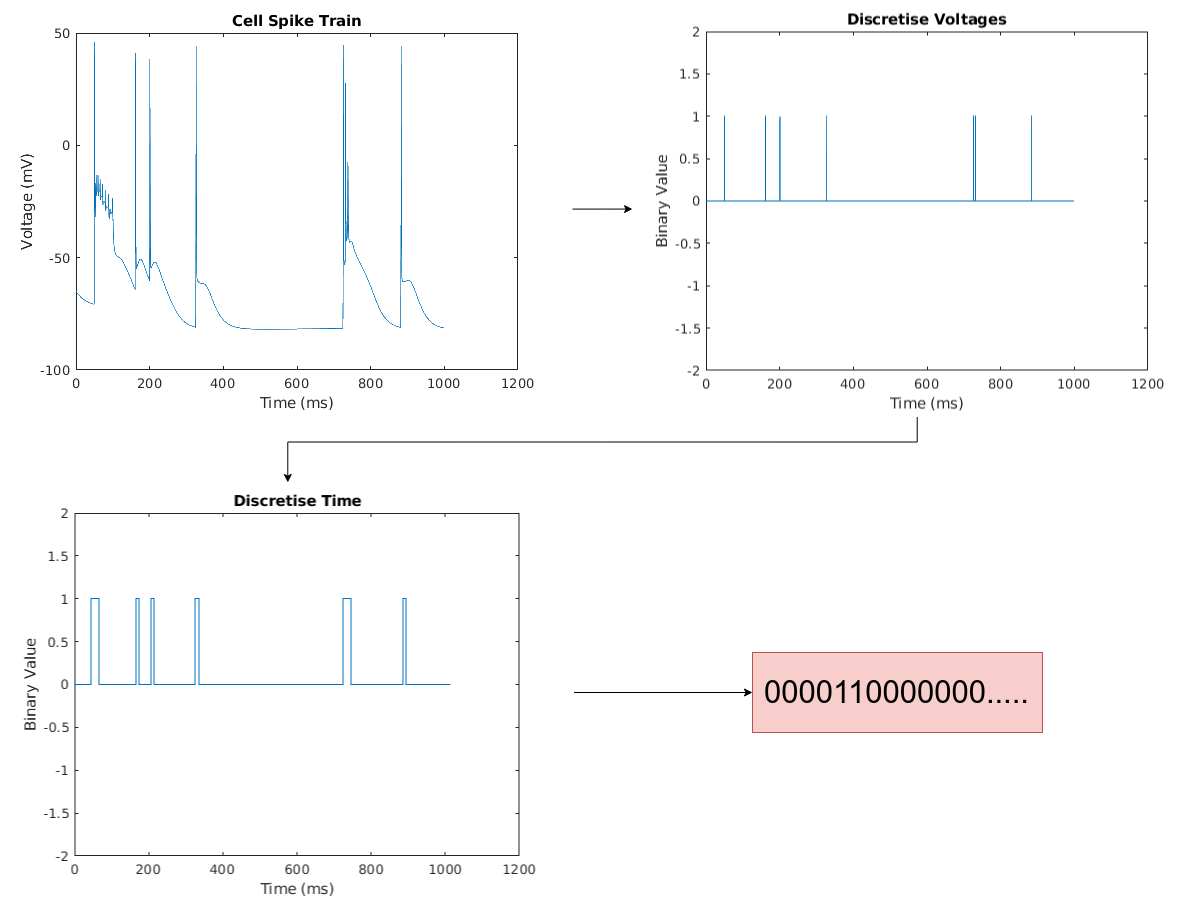
\includegraphics[width=\textwidth]{04-Methodology/descrTrain.png}
    \caption{Process of spike-train discretisation}
    \label{fig:discrTrain}
\end{figure}
The binary output sequence of this process represents the symbol of the system; in this case our symbol is 1 bit and so our symbol set can be described as $S=\{s_{1}=0, s_{2}=1\}$. Here we can calculate the binary sequence from the head cell (which we can represent as a random variable $X$) as well as from the tail-cell (represented as random variable $Y$) With this in mind, we can use the equations described in Section \ref{chap:back:infTheory}, specifically equations \ref{eq:entropyDiscr} and \ref{eq:mutualInf} to calculate the entropy of the head-cell and mutual information of the cortical link. The probability mass function (PMF) of both X and Y (that is, $P(X)$ and $P(Y)$) can be calculated from their respective binary sequences. We can then apply various forms of Baye's rule, along with further analysis of the two binary sequences, to obtain the joint PMF ($P(X,Y)$) and the conditional PMF ($P(X|Y)$) for use in the calculation of the mutual information of the cortical link.

\subsection{Delay Estimation}
For the estimation of the cortical link, we employ a simple cross-correlation analysis. The cross-correlation function describes the relation between two signals across a series of time shifts, and is described by
\begin{equation}
    \label{eq:xcorr}
    r_{xy}(l) = \sum_{n=-L}^{L-1}x(n)y(n-l)
\end{equation}
where $r_{xy}$ is the cross-correlation of $x$ and $y$ and L is the number of lags (time shifts) to calculate for in the positive and negative direction. Conceptually, a spike in the head cell should result in a spike in the tail-cell separated roughly by the delay as the spike crosses the synaptic connection. As a result, we should find a peak in the cross-correlation between the voltage measurements of the two cells as the time shift approaches the delay since at this time-shift the signals should be relatively well correlated.\\
While this approach is quite basic and may not be overly accurate, it is a first step in expressing the characteristic function of the delay in the neuronal link, which is an important concept when applying network tomography to estimate link-level delay \cite{netTomFour},

\section{Cell Classification}
\subsection{Feature Extraction and LNP Estimation}
% TODO:Explanation of the process followed to estimate the LNP filter coefficients to a specified order, and other methods that this could be implemented (i.e. iterative rather than analytical).\\
% Discussion of other features that could be used.
As previously mentioned, the Linear-Nonlinear-Poisson (LNP) cascade model can be used to model and characterise the response of a neural cell. Generally, this is computed using the spike-triggered-average (STA) of the stimulus sequence \cite{lnpInBrain} however this approach is more appropriate when dealing with external stimuli such as a spatio-temporal screen.\\
For this reason, another approach was taken to estimate some of the parameters of the LNP model. As we are not intending to recreate the spike train of the neuron, we can disregard the Poisson-spike generation portion of the model. As well as this, in the interest of simplicity, we will disregard the nonlinear component as the linear component should have a higher proportion of the overall characterisation.\\
The problem in this case is then to calculate the linear filter that best represents the response of the cell, to a predefined number of filter coefficients. This is referred to as \emph{System Identification} \cite{sysIdA}\cite{sysIdB}. The theoretical principle here is: given the linear system 
\begin{equation}
    \label{eq:firLinSys}
    y = x \star h
\end{equation}
estimate the value of $h$ to a limited order that best produces the output sequence $y$ from input sequence $x$. If we take this to be representative of a finite-impulse response (FIR) filter, we can describe the system as

\[
\begin{bmatrix}
    y_{0} \\
    y_{1} \\
    y_{2} \\
    y_{3} \\
    \vdots \\
\end{bmatrix}
=
\begin{bmatrix}
    x_{0} &    0  &    0 &     0  &    0 \\
    x_{1} & x_{0} &    0 &     0  &    0 \\
    x_{2} & x_{1} & x_{0} &    0  &    0 \\
    x_{3} & x_{2} & x_{1} & x_{0} &    0 \\
    \vdots & \vdots & \vdots & \vdots & \vdots \\
\end{bmatrix}
\begin{bmatrix}
    h_{0} \\
    h_{1} \\
    h_{2} \\
    h_{3} \\
    h_{4} \\
\end{bmatrix}
\]
for a sample 5-order filter \cite{sysIdC}. This system is not invertible to solve for $\vec{h}$ as $\boldsymbol{X}$ is not square, it is possible to solve for $h$ under "general conditions" through the use of the \emph{pseudoinverse} of $\boldsymbol{X}$. This can be more specifically defined by the Moore-Penrose pseudoinverse of $\boldsymbol{X}$, so $\vec{h}$ is given by
\begin{equation}
    \label{eq:estFilter}
    \vec{h} = (\boldsymbol{X}^{T}\boldsymbol{X})^{-1}\boldsymbol{X}^{T}\vec{y}
\end{equation}
where $\vec{h}$ is the estimated filter, $\boldsymbol{X}$ is the equivalent time-delayed input matrix, and $\vec{y}$ is the output signal vector. This approach is relatively computationally complex, especially for larger signals and alternative approaches do exist in the estimation of filter components through iterative means, however for this application at this scale there were no major issues found.

\subsection{Classification Tools}

To investigate the classification of neuronal cells (and to compare the performance of the different classification algorithms), two analytical tools were used: Matlab, and RapidMiner.\\

\begin{figure}[ht]
    \centering
    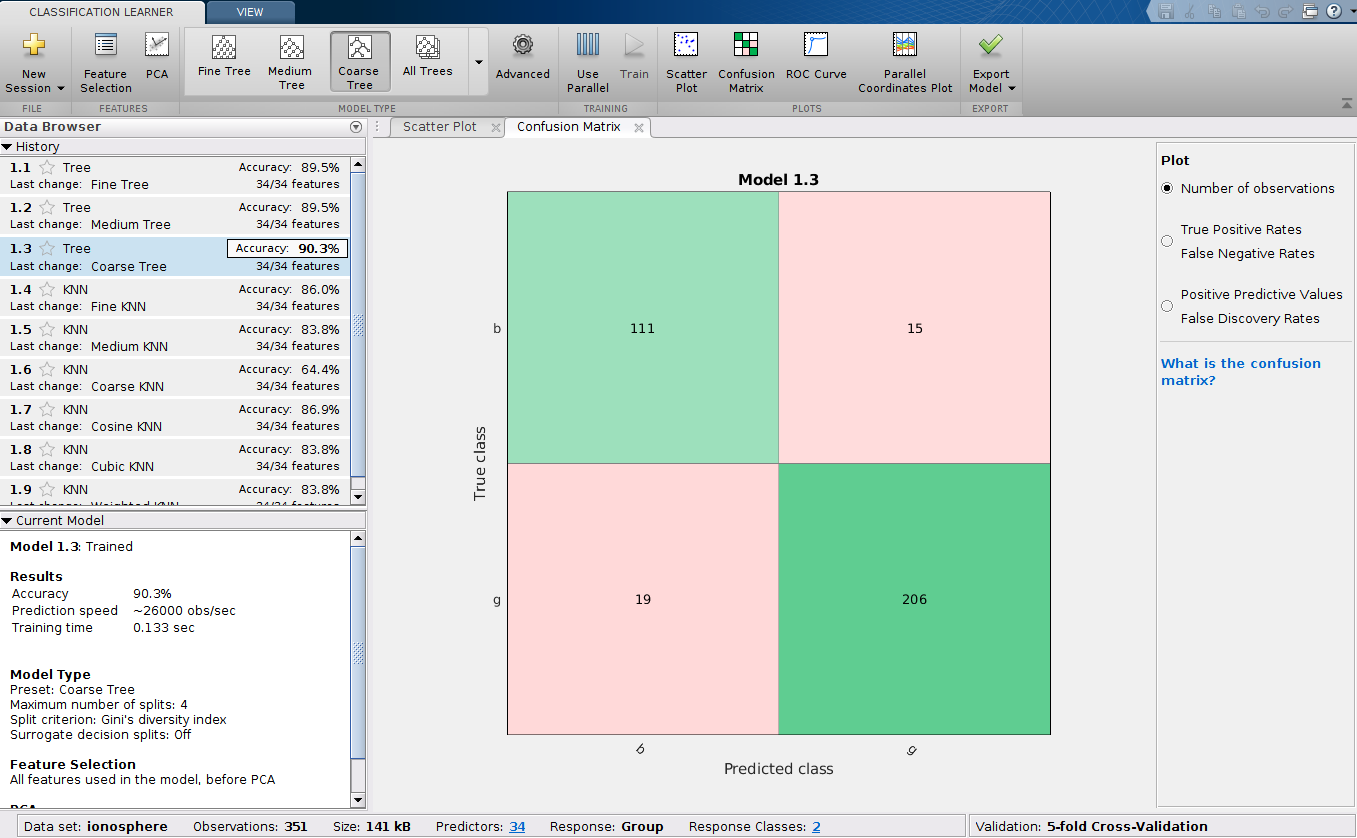
\includegraphics[width=\textwidth]{04-Methodology/mlClassificationLearner.png}
    \caption{Classification example in Matlab}
    \label{fig:classLearnerSamp}
\end{figure}
Matlab is a tool widely used for the numerical analysis of data and offers a wide range of additional add-ons, a large community backing, and an efficient backend. One of the add-ons available in Matlab is the \emph{Classification Learner}. This is a tool that takes a dataset as input, requests the specification of the features and classes in the dataset, and then quickly trains a number of different classifiers against the data, reporting the individual classifier accuracy, confusion matrix, and receiver-operating-characteristic (ROC) curve. This tool is therefore very useful for quickly getting an idea of how the different forms of classifier are dealing with the given features and classes. A diagram of the Classification Learner tool in use is shown in Figure \ref{fig:classLearnerSamp}. Here the comparison between the classifiers can be seen, along with the confusion matrix for one of the classifiers.\\

\begin{figure}[ht]
    \centering
    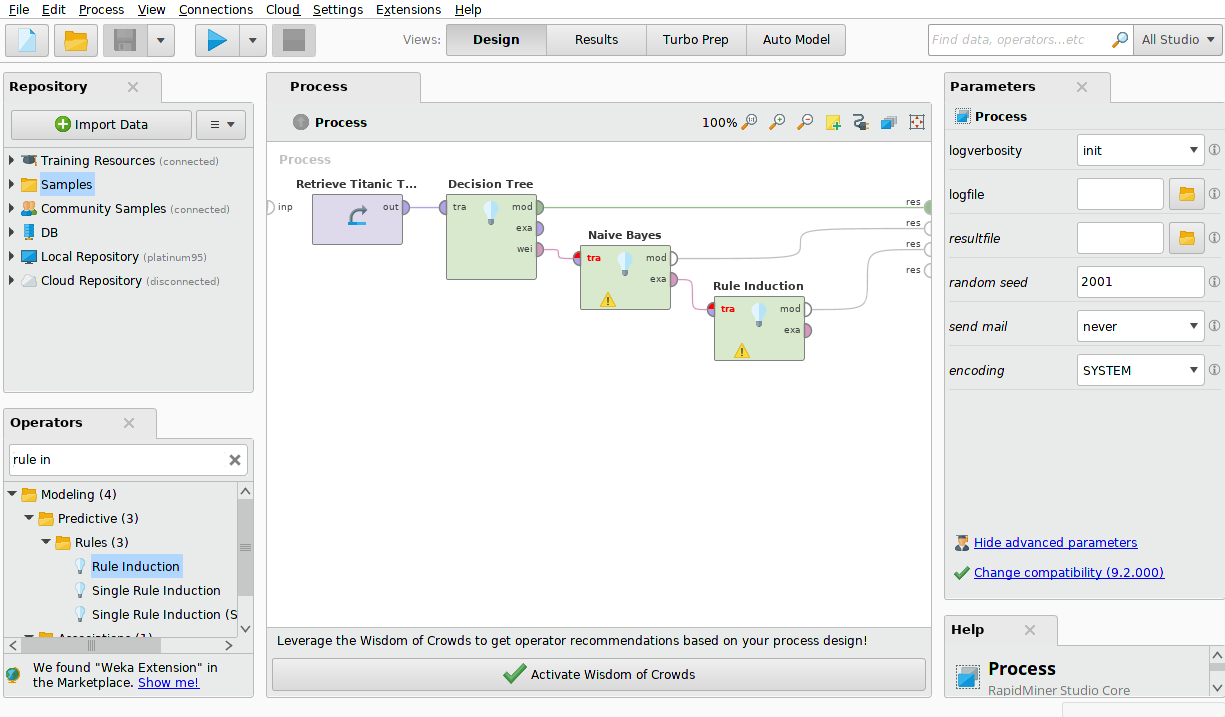
\includegraphics[width=\textwidth]{04-Methodology/rapidMinerUI.png}
    \caption{Classification example in RapidMiner}
    \label{fig:rapidMinerUi}
\end{figure}
For more fine-grained control of the classifier parameters, RapidMiner was used. RapidMiner is a tool that is used in "Big Data" for the analysis of large sums of data. It features a node-link type graphical interface in which the user can construct data processing pipelines involving various stages of data passthrough, as well as a wide range of classification and machine-learning algorithms. A diagram of the user interface of RapidMiner with an example data-processing pipeline is shown in Figure \ref{fig:rapidMinerUi}.\\

%TODO: Fill out this section with the specific layout of the rapidminer pipeline used for classifying.

\subsection{Cell-Type Segregation}
% TODO: Discussion of the splitting of a given cell into associated layer, m-type, and e-type to make classification easier.\\
% Discussion of the classifier stacks (i.e. output of layer-classifier as input to m-type classifier etc) and why this was done (layer/m-type/e-type not mutually independent).
We have previously discussed how each of the cells in the dataset has been classified by the BBP; that is, each cell has an associated layer, m-type, and e-type. As there are over 1000 individual cell models, it is unlikely that a classifier will be capable of gaining any form of functional accuracy in directly classifying the exact cell type. For this reason, the classification of a given cell was broken down in the classification of each of its constituent components, i.e. 3 separate classifiers were trained to estimate the cell type. The first classifier estimates the layer to which the cell belongs based on the filter coefficients extracted through equation \ref{eq:estFilter}. The second classifier estimates e-type based on the filter coefficients as well as the output of the first classifier (the layer estimation). The final classifier estimates m-type based on the filter coefficients, the estimated layer, and the estimated e-type. In this format, each classifier is only estimated against 5, 11, and 24 classes respectively. The other benefit of this approach is that the output of one classifier can be fed into the next, which allows the classifier to take into account the associated probability of one class leading to another, for example it might be more likely that layer 1 neurons contain more pyramidal m-types.\\
For training the classifiers, therefore, the "simulated cell" class will be broken down based on the cell identifier string. By splitting the string at all underscore characters ("\_") we can reliably extract the three constituent classes. For example, taking the cell identified by "L1\_DAC\_bNAC", splitting the string at all underscores results in three substrings, \{"L1", "DAC", "bNAC"\}, which correspond to the classes \{layer, m-type, e-type\}.

\subsection{Network Topographies and Tomography}
%Types of networks analysed (2-cell to train, 4-leaf to test tomography).
%Discussion on the tomography of the reconstruction of the cell-types, i.e. applying the pre-trained models to the 4-leaf network to estimate the cell-type of the leaves.
There are two main topologies investigated in this study: 2-cell topology, and 4-leaf star topology.
\par
\begin{wrapfigure}{R}{0.3\textwidth}
    \begin{center}
        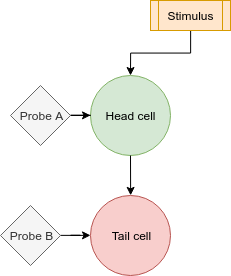
\includegraphics[width=0.3\textwidth]{04-Methodology/2cellTop.png}
    \end{center}
    \caption{2-cell Topology}
    \label{fig:2cellTop}
\end{wrapfigure}
The 2-cell topology is shown in Figure \ref{fig:2cellTop}. This 2-cell topology is quite simple as it is used mainly to analyse the link between two neurons rather than to study the various effects of neuronal layout. It consists of two cells linked by a synaptic connection whose parameters vary between network to network. A probe is attached to each cell to measure the output spike trains at all times in the simulation. A stimulus is also connected to the "head" node, whose parameters also vary between simulation to simulation.

\par


The 4-leaf star topology is shown in Figure \ref{fig:4leafStar}. This is a slightly more complex network than the 2-cell topology. The intention of the use of this network is to analyse the application of the results found from the study of the 2-cell networks in more complex topologies to investigate what effects, if any, the topology may have on performance. It is important to note here that the direction of the synaptic connections is that of an "out-hub", i.e. the central node (acting as the hub) is delivering voltage spikes to the surrounding leaves. This is in contrast to the 4-leaf star layout previously analysed \cite{ekkyProj} where the 4-leaf star topology acted as an "in-hub" with the leaf nodes delivering spike-events to the central node.
\begin{figure}[ht]
    \centering
    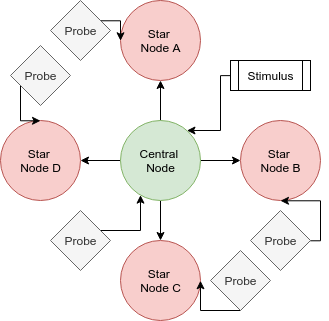
\includegraphics[width=0.5\textwidth]{04-Methodology/4cellTop.png}
    \caption{4-leaf star Topology}
    \label{fig:4leafStar}
\end{figure}
\par

For the investigation of the neuronal classification, the topologies will be used in the following manner. The voltage measurements taken from the database of 2-cell networks will be used to train the classification models, and to compare the performance difference between the different algorithms. When the classification models have been fully trained, they will be applied on the voltage measurements of the 4-leaf star topology simulations. The classifier will then attempt to estimate the type of cell used in each leaf node in order to reconstruct the topology; in other words, the classifier will be used to apply network tomography to estimate the parameters of the 4-leaf star network from a number of endpoint measurements. The performance of the classifier in this application will be compared against the performance in the 2-cell networks and differences will be discussed (if any).

\chapter{Results}
\label{chap:res}
\section*{Chapter Outline}
In this chapter we present the results generated from the various experiments. We first present the results of the link-level delay estimation using cross-correlation and show the analysis of the performance of this estimator. We then present the results of the investigation of the mutual information between two cells, and show how there is little to no correlation between the link-parameters and the calculated results. Finally, we present the results of the cell-classification model, and compare the performance of the various classifiers.


\section{Neuronal-Link Parameters}
% \begin{itemize}
%     \item Some graphs of the stimulus/response spike-trains
%     \item Some graphs on the discretisation of a spike train into a binary sequence.
%     \item Some plots of the estimated mutual information vs network parameters
%     \item R-scores of the correlation between the mutual information and the parameters
% \end{itemize}
% TODO: bad results cos not enough data? Cite da paper.

\subsection{Delay Estimation}
As stated in \ref{chap:meth:llMeth}, the analysis of the link-level details of a synaptic connected was done through the simulation of around 10,000 simple 2-cell networks. This results in the production of sets of voltage data for each simulation, one from the "head" cell and one from the "tail" cell. As the output of one cell is acting as the stimulus to the other, the spike trains from the simulations tend to be correlated. The output plots of a number of a few of these simulations is shown in Figure \ref{fig:sample2CellPlots}. In these sample plots, the source-destination spike correlation is clear to see as a spike in the pre-synaptic cell often results in a spike in the post-synaptic cell. As well as this, the plots indicate a slight delay between the source and event spikes.
\begin{figure}[ht]
    \centering
    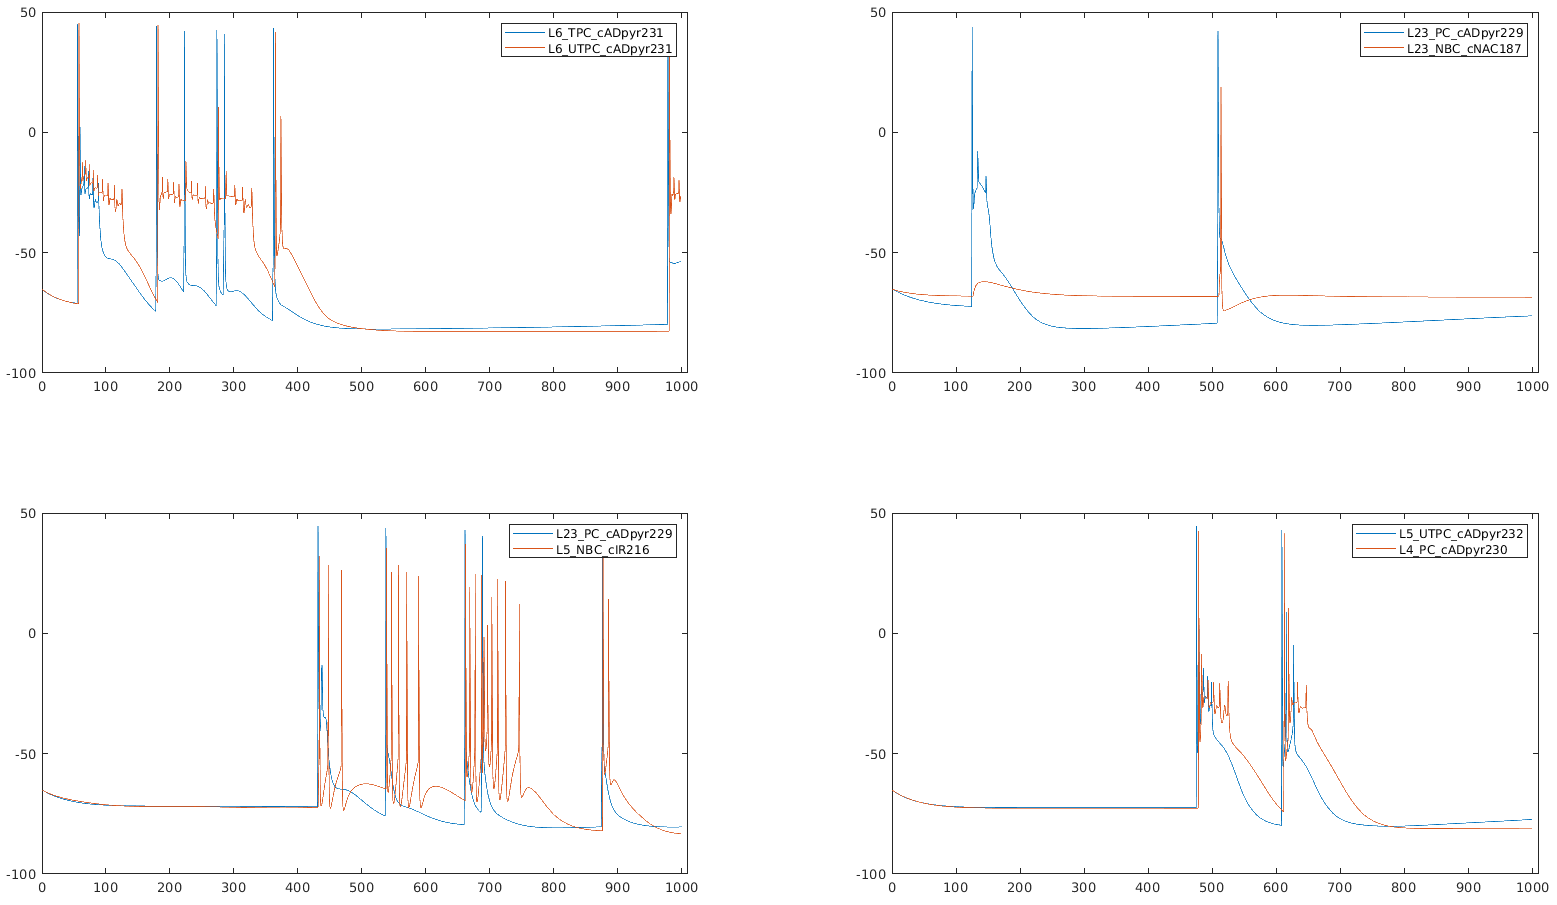
\includegraphics[width=\textwidth]{05-Results/2cellComp.png}
    \caption{Comparison of 2-cell network outputs. Head cell in blue, tail cell in orange. Cell-types shown in each subplot's legend}
    \label{fig:sample2CellPlots}
\end{figure}

\par

Following the collection of the simulation data, analysis was done on the estimation of the link delay through the use of the cross-correlation between the two measured voltage plots. This was implemented by loading the two cell voltage series, and using the Matlab \emph{xcorr()} function to get the cross-correlation of the two series to a specified number of lags. Next, we find the closest positive peak in the cross-correlation using the \emph{findpeaks()} function. This function finds the local maxima in a series which are the portions of the plot where the first derivative is 0 and the second derivative is negative (concave-down). By making the assumption that the first local maxima represents the delay, we can obtain a simple estimate of the link delay. Figure \ref{fig:sample2CellCorrPlots} shows a number of plots representing this delay estimation. Each subplot shows the cross-correlation of the 2 signals at a number of lag values from -12ms to +12ms, along with the location of the estimated link delay (i.e. the location of the first positive peak) and the location of the actual link delay (as specified by the \emph{delay} parameter in the associated \emph{NetCon} object.\\

\begin{figure}[ht]
    \centering
    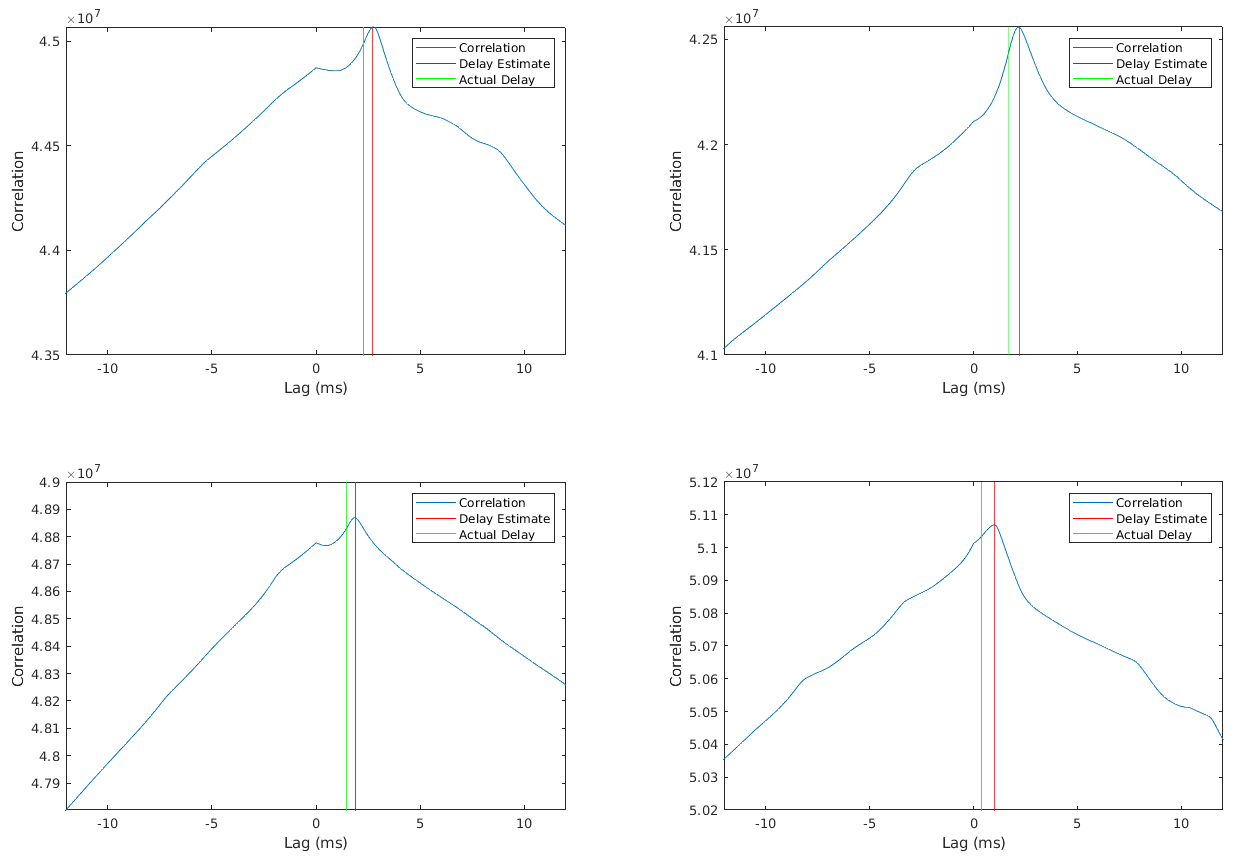
\includegraphics[width=\textwidth]{05-Results/2cell_Corr.png}
    \caption{Comparison of 2-cell cross-correlation with delay estimate. Cross-correlation shown in blue, estimated delay as a vertical red line, actual delay as a vertical green line}
    \label{fig:sample2CellCorrPlots}
\end{figure}

With this method of delay estimation, the estimator was run against all the simulated networks (N=10,000) and the correlation between the estimated delay and the actual delay was analysed. First, the estimations of 0ms were removed, as this was the "error value" returned by the estimator when it was unable to determine the actual delay (possibly due to a lack of spike-data in the simulation). A linear model was then fit to the data in order to determine the correlation between the estimation and the actual delay. A scatter-plot of the estimation and actual delay is shown in \ref{fig:2CellDelayLFit} along with the least-squares linear fit and associated R-squared score. The mean-squared error of this linear model was 1.0881.
\begin{figure}[ht]
    \centering
    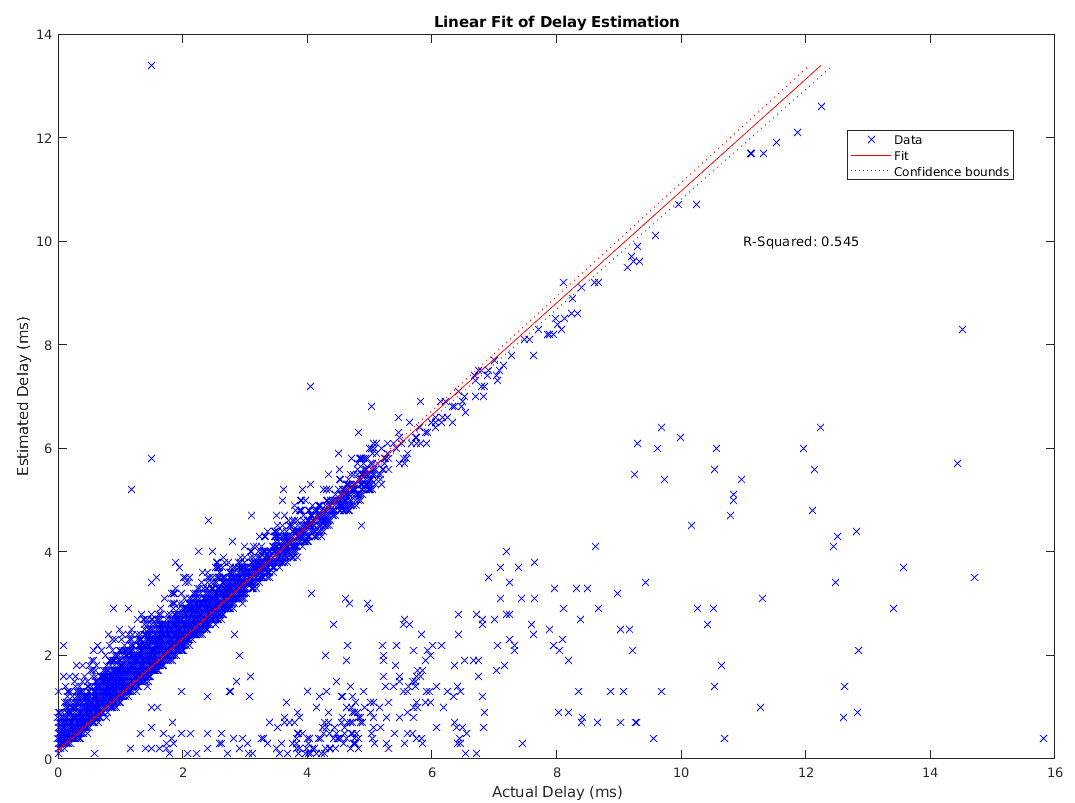
\includegraphics[width=0.8\textwidth]{05-Results/delayFit.png}
    \caption{Correlation of delay estimate vs actual delay with least-squares linear model and associated R-squared score}
    \label{fig:2CellDelayLFit}
\end{figure}

\subsection{Entropy and Mutual Information}
As discussed in \ref{chap:meth:llMeth}, the entropy of the cells is calculated by discretising the spike train and treating it as though the spikes represent a single binary symbol. The process for this is outlined in \ref{fig:discrTrain} and was again implemented in Matlab. Using the symbol sequence it is then possible to apply the corresponding equations (\ref{eq:entropyDiscr}, \ref{eq:mutualInf}) to determine the entropy of the individual cells, and the mutual information of the cell-to-cell connection. As well as this, we can use the delay estimation model described above, which allows us to shift the spike train of the "tail" cell such that the spike-response should be instantaneous. This is done to investigate whether or not adjusting for the delay in the link will effect the calculated mutual information.\\
The probability-mass function (PMF) of the calculated single-cell entropy is shown in Figure \ref{fig:cellEntPmf}. The majority of the cells have an entropy of below 0.4 bits/symbol, with a continuously decreasing proportion of the cells having an increasing entropy. The PMF of the calculated mutual information is shown in Figure \ref{fig:mutualInfoPmf}. We can see that the mutual information of the networks is well-distributed, with a mean of around 0.5 bits. Of note here is that the effect of shifting the spike-train based on the delay estimate has little to no effect on the distribution of the mutual information. \\

\begin{figure}

\centering
\begin{subfigure}[b]{0.9\textwidth}
    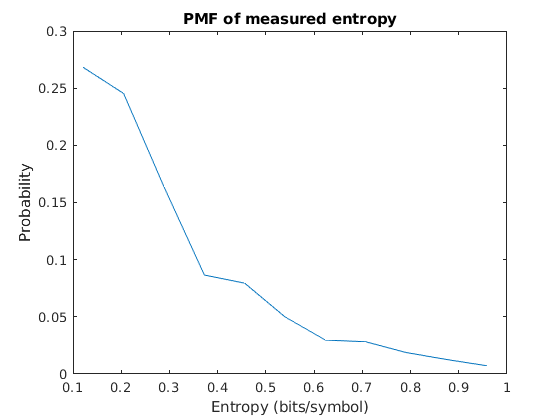
\includegraphics[width=1.0\textwidth]{05-Results/entropyPmf.png}
    \caption{PMF of calculated single-cell entropy based on output spike trains}
    \label{fig:cellEntPmf}
\end{subfigure}

\begin{subfigure}[b]{0.9\textwidth}
    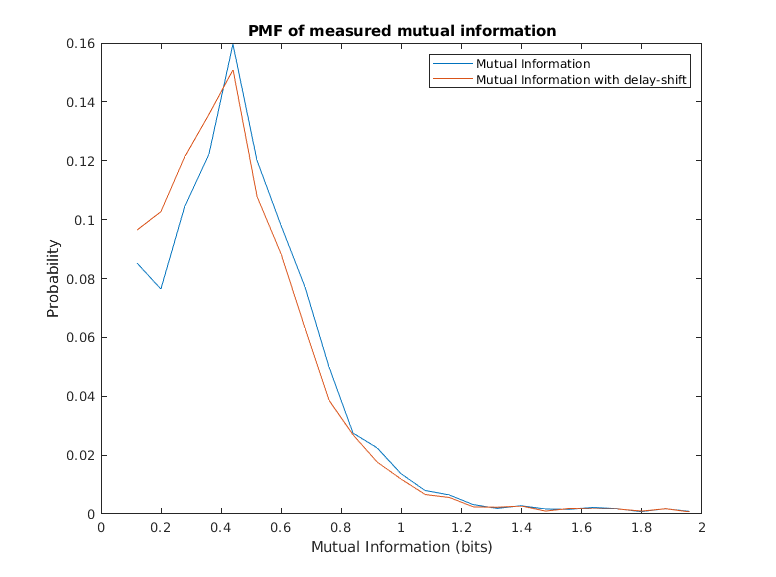
\includegraphics[width=1.0\textwidth]{05-Results/mutualInfo_pmf.png}
    \caption{PMF plots of calculated mutual information for the measured spike-train (blue) and the delay-estimate shifted spike-train (orange)}
    \label{fig:mutualInfoPmf}
\end{subfigure}
\caption{PMF of 2-cell entropy and mutual information}
\end{figure}


% \begin{figure}[ht]
%     \centering
%     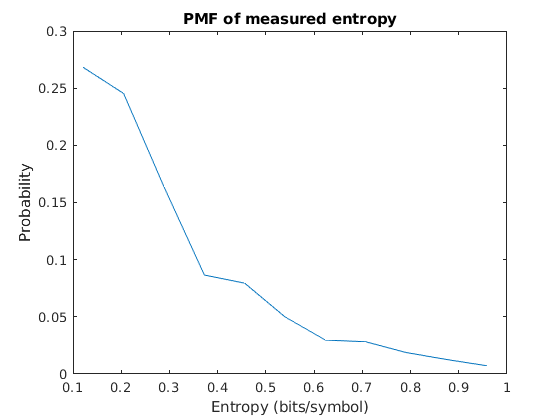
\includegraphics[width=0.9\textwidth]{05-Results/entropyPmf.png}
%     \caption{PMF of calculated single-cell entropy based on output spike trains}
%     \label{fig:cellEntPmf}
% \end{figure}

% \begin{figure}[ht]
%     \centering
%     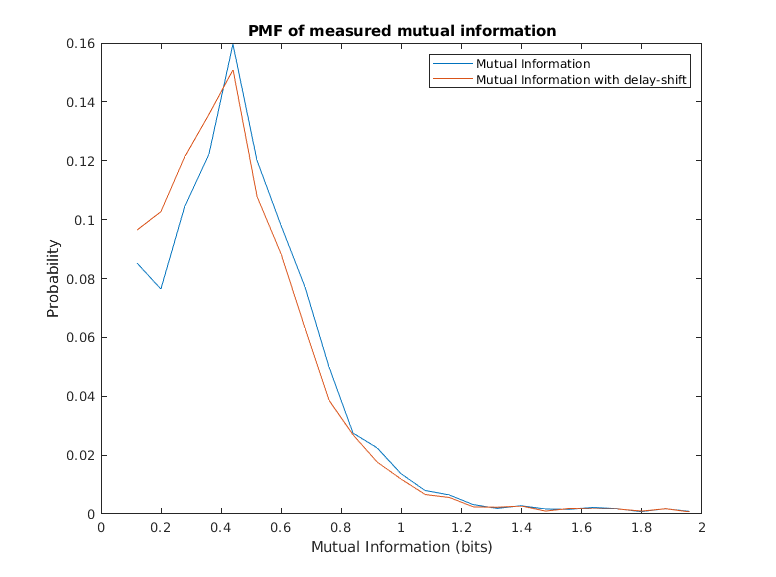
\includegraphics[width=0.9\textwidth]{05-Results/mutualInfo_pmf.png}
%     \caption{PMF plots of calculated mutual information for the measured spike-train (blue) and the delay-estimate shifted spike-train (orange)}
%     \label{fig:mutualInfoPmf}
% \end{figure}

We next look at the possible factors that may have an effect on the mutual information. We can plot a number of scatter-graphs to visually represent any correlations in the data, as shown in Figure \ref{fig:mInfoCorrGraph}. In this figure, we can examine any correlation between the mutual information and the number of synapses in the connection, the delay in ms of the link, the weight of the link, and the distance between the 2 cells in the network. We can see that there is no obvious correlation between any of the link-level parameters and the mutual information of the network.\\
\begin{figure}[ht]
    %\centering
    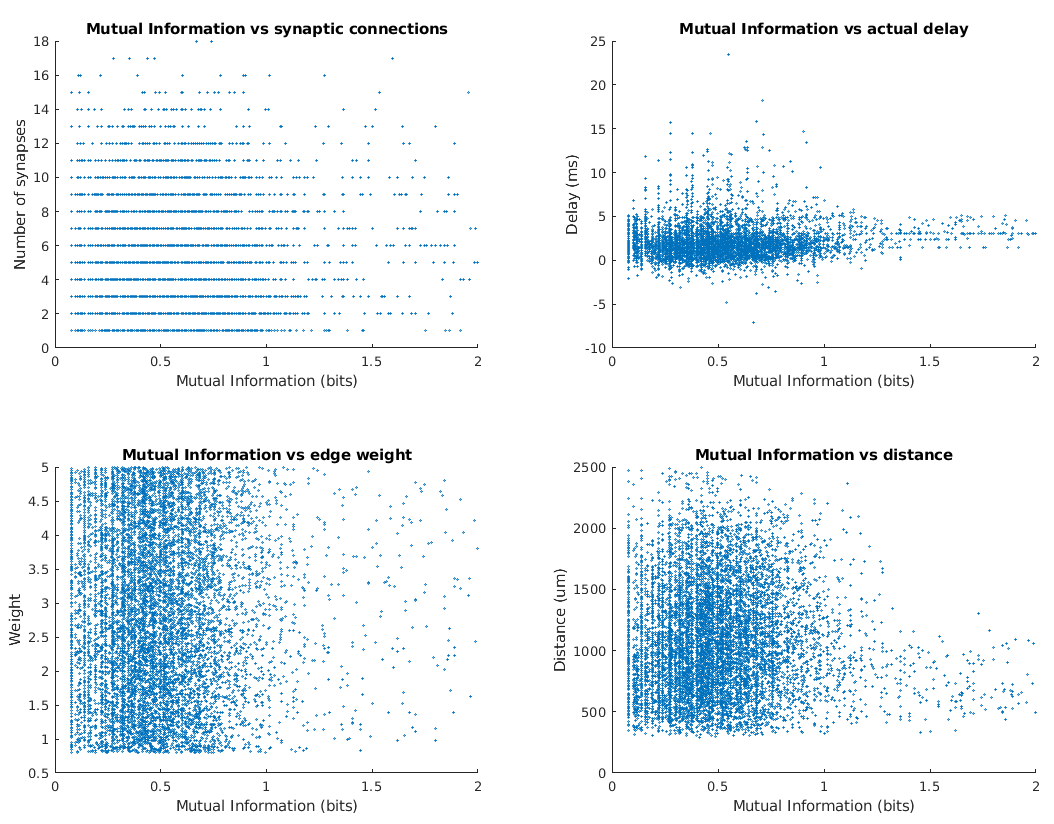
\includegraphics[width=\textwidth]{05-Results/minfoCorrPlot.png}
    \caption{Scatter plots of measured mutual information vs number of synapses, edge delay, edge weight, and distance between the cells.}
    \label{fig:mInfoCorrGraph}
\end{figure}
While there is no obvious correlation between any single parameter and the mutual information, these 2-d plots do not take into account all of the link parameters at once; that is, it could be that correlation could be found by analysing the dimension-space made up of all measured parameters. This can be done using a linear model, as used to determine the correlation in the delay estimate. In this case, we use multiple predictor variables (the link parameters) and a single response variable (the mutual information). This model is shown in Figure \ref{fig:lmInfo}. With an R-squared score of 0.034, it is clear that there is no correlation between the network parameters and the mutual information of the neural link.
\begin{figure}[ht]
    \centering
    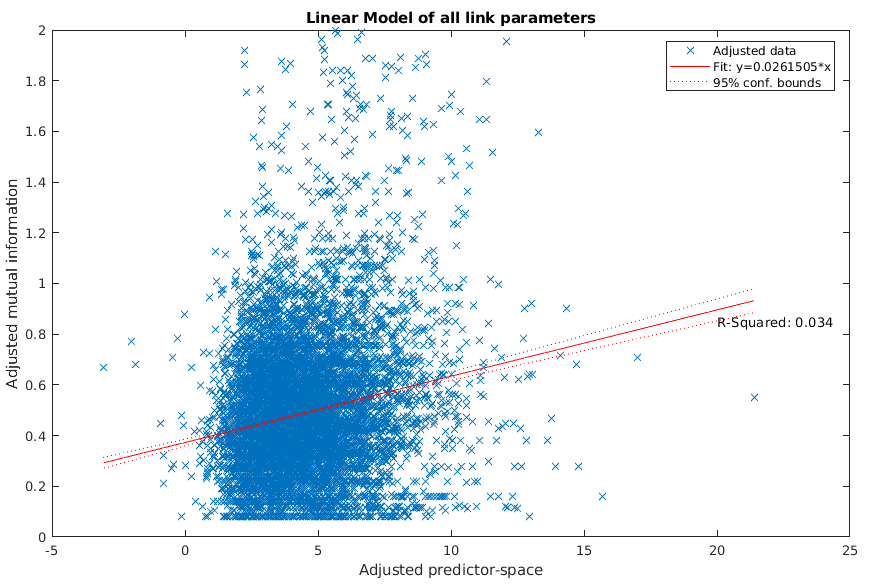
\includegraphics[width=\textwidth]{05-Results/lmMinfo.png}
    \caption{Linear fit of all network parameters to predict mutual information}
    \label{fig:lmInfo}
\end{figure}


\section{Classification}

\subsection{2-Cell Classification and Model Training}
% \begin{itemize}
%     \item Spike train figures showing the difference in impulse response between cells
%     \item Some figures of the LNP estimation and associated coefficients
%     \item Some scores on the separation of the filter coefficients between cell classes
%     \item Confusion matrices and different model metrics for the classification models, and the differences in the analysed algorithms (GMM, SVM, NN etc)
% \end{itemize}
% TODO: above

In Figure \ref{fig:sample2CellPlots} a number of spike-trains from different cell types were shown. Referring back to this, it is clear that different cells respond different to stimulus, with the output spike train differing in intensity (frequency of spikes) as well as in the "settle-down" period after a spike was triggered (i.e. the fall-time response of the membrane voltage). It is these differences that we attempt to characterise through the use of the linear-filter portion of the linear-nonlinear-Poisson (LNP) cascade model.\\
The first step in this process is to simulate a number of 2-cell networks again in order to generate test data. In this instance, the "head" cell acts only as a stimulus generator, and we treat the soma-membrane potential of this cell as the "input" voltage to the linear system described in \ref{eq:firLinSys}. In order to limit the number of variables in this investigation, the type of cell used as the head cell was constant across all simulations (layer 1, DAC m-type, bNAC e-type) while the "tail" cell was treated as the cell-under-test and so was varied between simulations. As well as this, variations in link-level parameters (number of synapses etc.) were kept to a minimum to reduce the number of variables. A large number of networks were generated (N=30,000) in order to produce a dataset of sufficient size for classifier training.
Following simulation and prior to training the classifiers, the filter estimation step described in equation \ref{eq:estFilter} was applied to extract the filter coefficients as features from the cell-response data. Figure \ref{fig:sampImpRes} shows the filter coefficients (FIR impulse response) of 4 different cells, with a filter-order of 64. It is clear from this diagram that the impulse-response estimation of the neuronal cell is capable of differentiating between the cell types. Using these estimated filter coefficients, we are now able to begin training the classifiers.
\begin{figure}[ht]
    \centering
    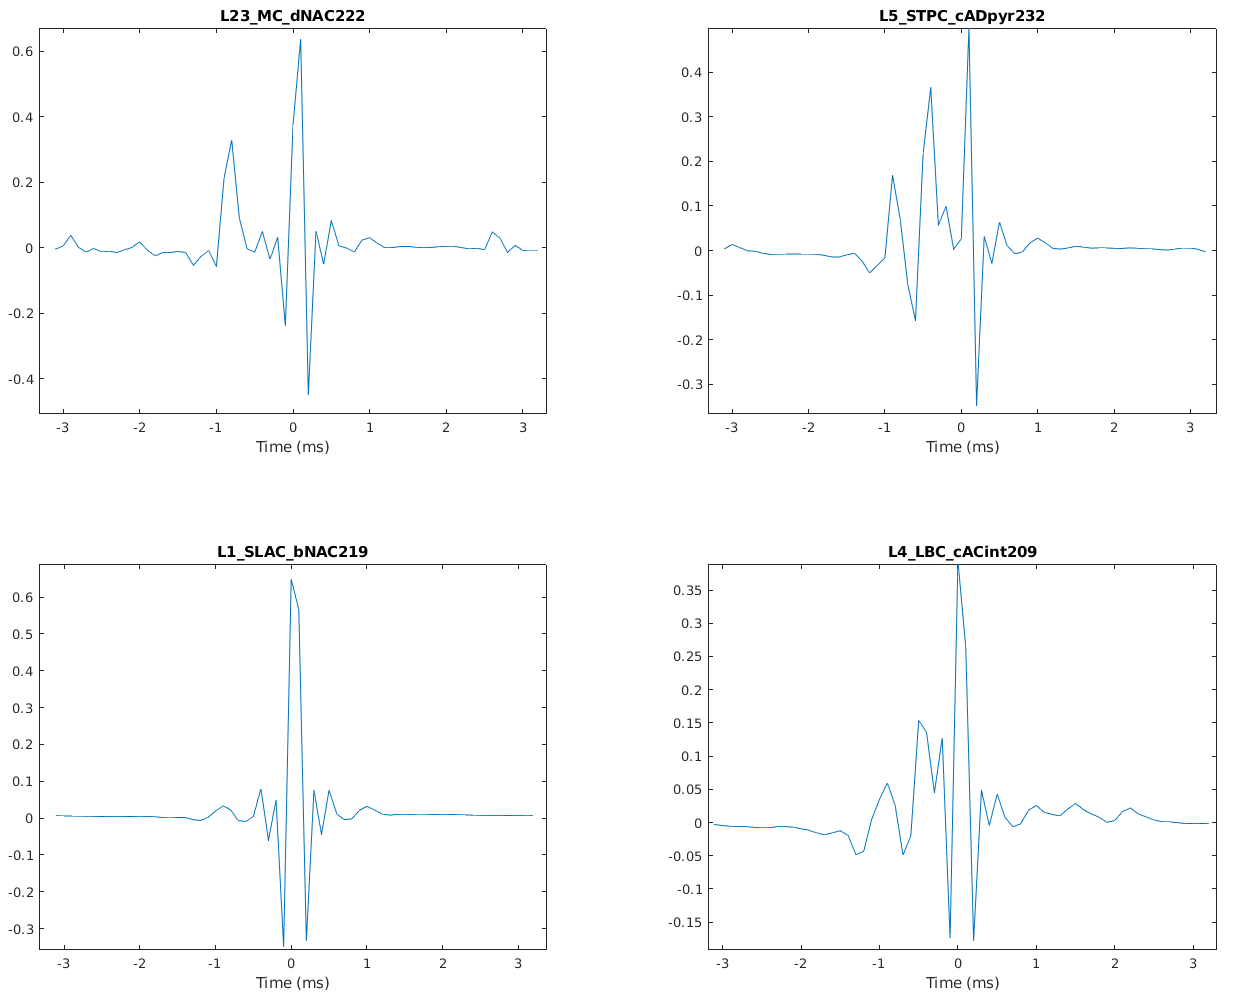
\includegraphics[width=\textwidth]{05-Results/sampImpRes.png}
    \caption{Sample impulse-response characterisation of different cells}
    \label{fig:sampImpRes}
\end{figure}

\par

Using the previously discussed \emph{Classification Learner} tool in Matlab, we can quickly train and compare a set of different classifiers, inspecting the accuracy, confusion matrix, and receiver-operating characteristic (ROC) curve for each. The first classifier to investigate is the layer classifier, which takes the estimated filter coefficients as input, and attempts to estimate what layer the characterised cell belongs to. Of the classifiers discussed in \ref{chap:back:class}, we can train and analyse SVM and Decision Tree classifiers. Using RapidMiner, we can also train artificial neural networks (NN), and the Random-Forest variation of the Decision Tree classifier.\\
The performance of the classifiers are shown in the following tables. In each table, we compare the performance of the different classification algorithms (Decision Tree, SVM etc.) in the classification of the separate cell sub-group types (layer, m-type, e-type). For each classifier we state the corresponding accuracy. The accuracy is calculated as the ratio of correct estimations versus incorrect estimations. We also state the "factor improvement" of the classifier. This is calculated as the factor by which the classifier improves over the equivalent accuracy of random guessing in the classification space. For example, with 5 layer classes the equivalent "random guess" accuracy is 20\%, and so a trained classifier with accuracy of 40\% would have a factor improvement of 2. \\

Table \ref{tbl:layerClassifierPerf} shows the performance of the classifiers in the prediction of cell layer-type, table \ref{tbl:mtypeClassifierPerf} for m-type prediction, and table \ref{tbl:etypeClassifierPerf} for e-type prediction. In every case, the SVM classifier has the highest accuracy, with the NN being slightly behind. Of the tree-based classifiers, interestingly the decision tree based classifier has a consistently higher accuracy than the random forest classifier, despite the latter being a variant of the former. 


\begin{table}[h]
    \centering
    \begin{tabular}{|c||c|c|c|c|}
        \hline
        Classifier & Decision Tree & Random Forest & SVM & NN\\
        \hline\hline
        Accuracy & 52.2\% & 41.43\% & 62.5\% & 60.98\%\\
        \hline
        Factor Improvement & 2.61 & 2.07 & 3.13 & 3.05 \\
        \hline
    \end{tabular}
    \caption{Performance of different algorithms at classifying cell-layer (5 classes, 20\% equivalent random guessing accuracy)}
    \label{tbl:layerClassifierPerf}
\end{table}

\begin{table}[h]
    \centering
    \begin{tabular}{|c||c|c|c|c|}
        \hline
        Classifier & Decision Tree & Random Forest & SVM & NN\\
        \hline\hline
        Accuracy & 42.6\% & 35.07\% & 63.7\% &57.99\%\\
        \hline
        Factor Improvement & 10.65 & 8.77 & 15.93 &13.92\\
        \hline
    \end{tabular}
    \caption{Performance of different algorithms at classifying cell m-type (25 classes, 4\% equivalent random guessing accuracy)}
    \label{tbl:mtypeClassifierPerf}
\end{table}

\begin{table}[h]
    \centering
    \begin{tabular}{|c||c|c|c|c|}
        \hline
        Classifier & Decision Tree & Random Forest & SVM & NN\\
        \hline\hline
        Accuracy & 63.8\% & 54.47\% & 75.3\% &73.94\%\\
        \hline
        Factor Improvement & 8.93 & 7.63 & 10.54 &10.35\\
        \hline
    \end{tabular}
    \caption{Performance of different algorithms at classifying cell e-type (14 classes, 7.143\% equivalent random guessing accuracy)}
    \label{tbl:etypeClassifierPerf}
\end{table}

\par

Another set of results that are often used to quantify the performance of a classifier is the class precision and the class recall. The class recall is calculated per-class as the ratio of correct predictions of a class versus the number of observations of that class. The class precision is again calculated per-class as the ratio of correct predictions of a class versus the overall number of the classifier estimated that class.  As these metrics identify the performance of the model on a class-by-class basis, it results in a large number of individual values to compare. When we consider that we are comparing 3 estimator groups with a relatively high number of classes per group (5 for layer estimator, 25 for m-type, and 14 for e-type), as well as the fact that each estimator group must be compared against 4 different classification algorithms, it becomes difficult to critically compare the performance of each individual class. In general, however, when analysing such metrics from single classifier, a \emph{confusion matrix} is used. The confusion matrix of the SVM-based layer estimator is shown in Figure \ref{fig:svmConfMatLayer}. The confusion matrix tabulates the estimations of a given classifier as a grid of "True Class" versus "Predicted Class". In this way, it can show how often an observation of a given class is estimated as belonging to some other class. As such, the diagonal (shown as green in the confusion matrix figure) shows the proportion of the correct predictions in the validation set (where true class equals predicted class). The right hand bar shows the proportional difference of the \emph{true positive rate} and the {false negative rate}. This true-positive rate is equivalent to the class recall.\\
While the confusion matrices for every single classifier investigated in this study are not included, the relative proportions between them tend to be similar (i.e. very high prediction accuracy between layer 1 and layer 6, with reduced accuracy in the intermediate layers).

\begin{figure}[ht]
    \centering
    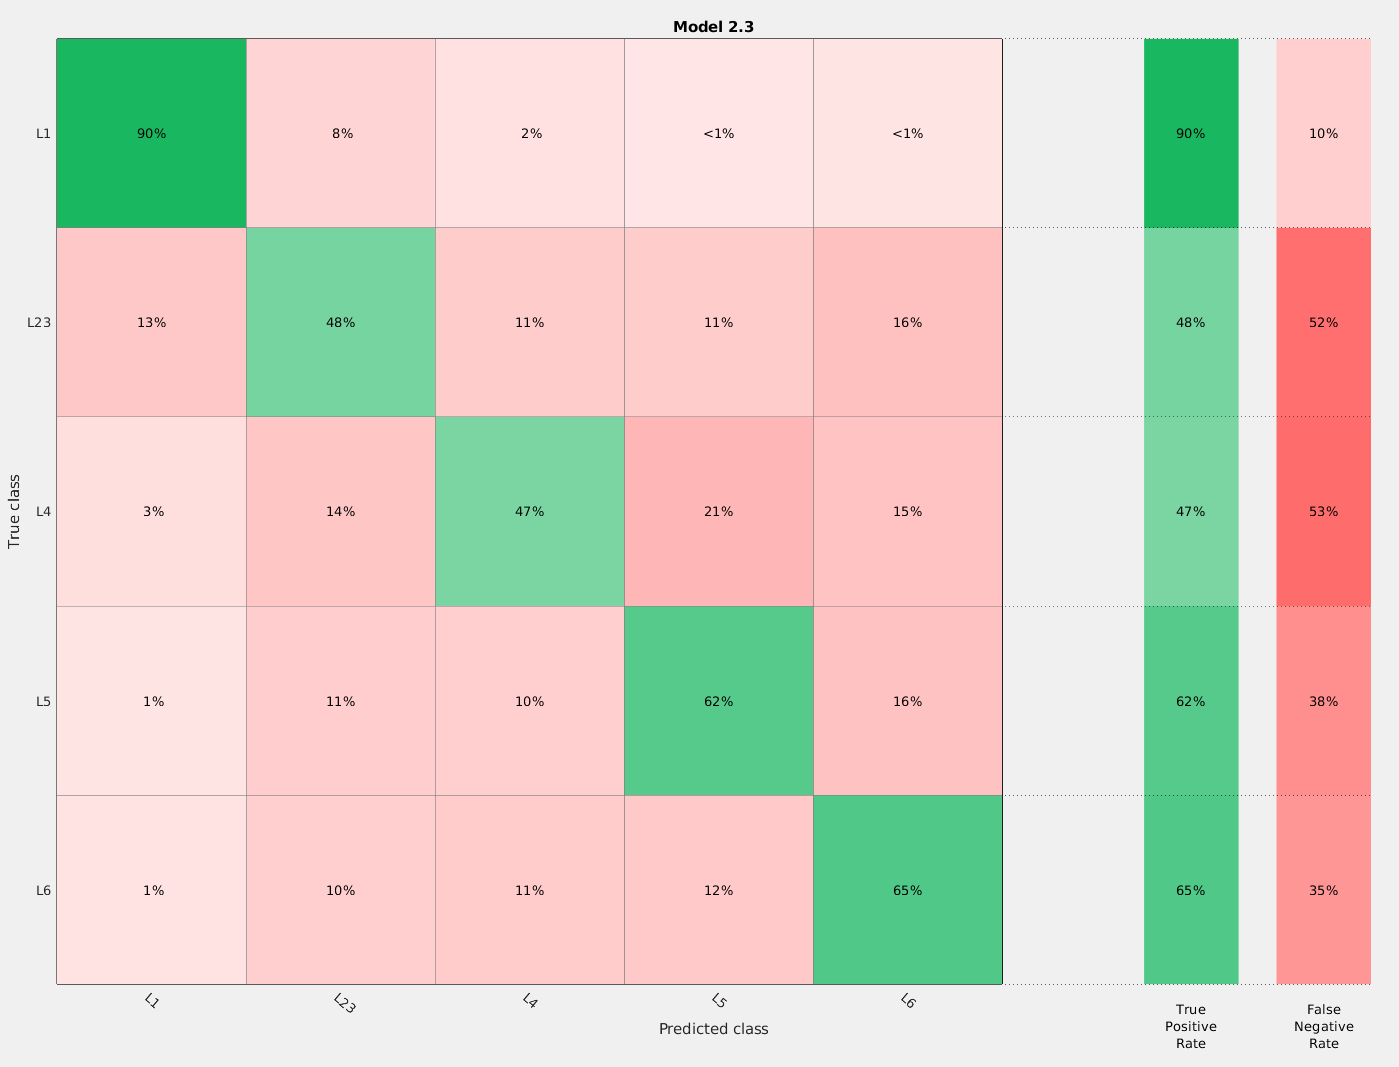
\includegraphics[width=1.0\textwidth]{05-Results/svmLayerConf.png}
    \caption{Confusion Matrix of SVM layer-classifier}
    \label{fig:svmConfMatLayer}
\end{figure}



\subsection{Network Tomography for Cellular Classification}
% \begin{itemize}
%     \item Figures of 4-leaf networks
%     \item Metrics in the reconstruction of these networks
%     \item Some figures showing the estimated network reconstruction vs actual network etc.
% \end{itemize}

As the SVM classifier had the best performance during training, this is the model that was applied in the reconstruction of the 4-leaf star networks. The process here was similar to the previous experiments: a number of unique networks were generated, simulated, and their data-points measured and analysed. In this case, the networks generated were of the 4-leaf star topology previously discussed and shown in Figure \ref{fig:4leafStar}. The central node was constrained to be of the same layer 1, DAC m-type, bNAC e-type cell type used in the training of the models, while the star cells were varied. For each measurement from the soma-membrane of a star node, the characteristic filter was estimated using the same process discussed previously, and the filter coefficients were passed through the pre-trained classifiers.

\par
The performance results of the topology reconstruction are shown in Table \ref{tbl:wholeClassifierPerf}. Here, we tabulate the accuracy of the classifier chain in estimating layer, m-type, and e-type groups, as well as the "whole-cell" classification accuracy. We define the whole-cell accuracy as the the cases where all three sub-groups were correctly estimated. Evidently, the factor-improvement for the whole-cell prediction is significantly higher than for any other group, while the sub-group accuracy is quite similar to those in the 2-cell networks.

\par

Figure \ref{fig:4CellRecon} shows a sample reconstruction of a 4-leaf network from probe measurements. The left side of the figure represents the network as it was simulated, with probes at the network endpoints and a stimulus on the central node, along with the actual cell types of the leaf nodes. The right side of the figure shows the reconstructed topology based on the cell-type estimations from the SVM classifier chain. 

\begin{figure}[ht]
    \centering
    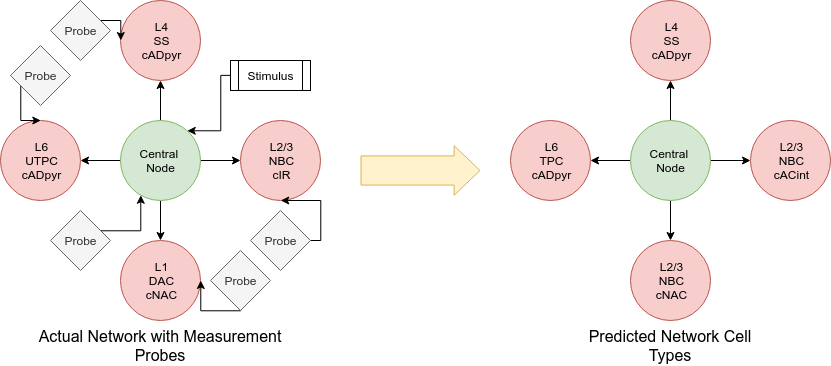
\includegraphics[width=1.0\textwidth]{05-Results/4cellTopRecon.png}
    \caption{Sample reconstruction of network}
    \label{fig:4CellRecon}
\end{figure}

\begin{table}[ht]
    \centering
    \begin{tabular}{|c||c|c|c|c|}
        \hline
        Prediction & Layer & m-type & e-type & whole-cell \\
        \hline\hline
        \# classes & 5 & 25 & 14 & 1750\\
        \hline
        Equiv. random guess accuracy & 20.0\% & 4.0\% & 7.143\% & 0.0571\%\\
        \hline
        Classifier accuracy & 61.82\% & 56.34\% & 64.62\% & 36.23\%\\
        \hline
        Factor improvement & 3.091 & 14.085 & 9.05 & 634.5\\
        \hline
    \end{tabular}
    \caption{Performance of 4-leaf star topology reconstruction}
    \label{tbl:wholeClassifierPerf}
\end{table}



\chapter{Discussion and Future Work}
\label{chap:disc}
\section*{Chapter Outline}
In this chapter we analyse and discuss the results presented in the previous section. We discuss the near-constant discrepancy between the estimated mutual delay and the ground-truth, and propose explanations for the low correlation in the mutual information investigation. We then compare the various cell-classifiers, discussing the difference between the algorithms' performance and the ability for the classifier to reconstruct a 4-leaf star topology. We also discuss areas that future research could investigate to improve on our findings. 


\section{Link-Level Analysis}
\subsection{Delay Estimation}


% TODO: Delay usually a bit high because the "actual" delay is from the netcon, not the netcon + synapse. Also measuring the cells output, not the cells input. The fact that there's a clear peak in the correlation for nearly every simulation with the estimate being nearly a constant overshoot shows that its measuring some form of delay, more like the propagation delay. Delays of 0ms were removed because error value. Delay fits well with a clear linear correlation between the actual delay and the estimate.\\
% TODO: Future work here could be on taking more than just the NetCon delay into account when getting the ground truth delay.

The delay estimation has proven to be quite accurate considering the relatively simple concept it is based on. While the estimated delay tends to be higher than the actual delay, the proportional difference between the two seems to be relatively constant meaning that a clear correlation can be seen, and that a simple linear model can fit with a decent R-squared score. This nearly constant difference between the estimation and the actual value can be explained by the nature of the simulation; the "ground truth" value taken as the network delay is the corresponding parameter applied to the \emph{NetCon} object connecting the two cells, while the measurements we take come from the soma of the two cells. This means that any delay we observe is from the delay of signal propagation through the axom of the presynaptic cell, through the NetCon object, across the synapse, and then through the dendrites of the post-synaptic cell. This means that any observed delay would be higher than the delay of just the NetCon object, which is supported by our data.\\
Another point of consideration in the delay estimation is that the estimator was not always able to predict a delay. This in general is due to the lack of peaks in the cross-correlation, which in turn may be caused by a lack of spikes in one or both of the voltage measurements possibly caused by a lack of synaptic connections. In these cases, the estimator returns a delay of 0ms. For this reason, any estimations of 0ms delay were simply removed from the dataset as they were assumed to have been caused by an invalid simulation.
\par
Future work in this area could take the whole delay path into account when forming the ground truth in the simulated network to verify the hypothesis that the estimation discrepancy is caused by this inaccurate ground truth. On top of this, the current model is quite simple in design and so could be improved upon to increase the robustness of the estimator to edge-cases where simple cross-correlation is not sufficiently accurate.

\subsection{Mutual Information}
% TODO: Discuss the results and how our analysis of the mutual information suggests this model isn't applicable to neurons.\\
% TODO: bad results due to lack enough data? Cite the paper that suggested this in their own study of the mutual information.\\
% TODO: Future work -> Discuss other models that may be applicable (i.e. the complex theoretical models given in other papers)\\

While the distribution of the measured mutual information in the simulation dataset does tend to follow a normal-like fit, it is clear from the various scatter plots that there is no correlation between the various link-level parameters between the cells and the discrete-memoryless model applied to the discretised spike trains. This lack of correlation is confirmed by the linear model which was "fit" to each of the link parameters, indicating a very low correlation with an R-squared score of only 0.03. This suggests that the application of the information model commonly used in digital systems is not sufficient to describe the information carried between cells through synaptic connections, possibly due to the fact that the transmission of a signal between two neurons is not entirely memoryless as the synapse has a refactory period during neurotransmitter reuptake. This could also be explained by a lack of sample data, as previous work done in this area has suggested that the accurate prediction of the entropy and mutual information of these links relies heavily on the size of the dataset, in particular of the length of the simulation and the number of spikes observed \cite{spikeTrainInfo}. As a result of this, future work in this area could investigate the effect of the simulation length and the activity within the simulation on the correlation between the calculated mutual information and the link parameters.\\
As well as this, other models could be applied in this domain to find the above parameter-information effect; for example, the calculation of upper and lower bounds on the mutual information as well as different approaches to the conversion between measured spike-trains and symbol sequences could be applied \cite{spikeTrainInfo}.

\section{Classification}
%TODO: Filter size discussion
%TODO: Classifier tweaking didnt change much -> could indicate we're at the limit of what the filter coeffs can tell us.
%TODO: Discuss the relatively good results and the differences between classifiers.\\
%TODO: Decision tree doing better than random forest? Possibly due to overfitting.
%TODO: Comment on our metrics, and why more metrics might be suitable.\\
%TODO: Discuss the better classification results between layers -> l1 v l6 etc\\
%TODO: Discuss the ability for the classifiers to identify layers vs m-types vs e-types.\\
%TODO: Good prediction for whole-cell -> might mean that predicting one correctly increases chance of predicting the other 2. Chaining effect?
%TODO: Good at classifying "similar" classes i.e UTPC classified as TPC, might be improved by better features.
%TODO: Accuract doesn't take probabilty into account.
%TODO: More m-types/etypes here than in list



The classification of cell types from measured membrane potential has shown promising results, with relatively high accuracy considering the high number of classes to which the models were estimating. Evidently, the SVM-based classifier had the highest level of accuracy, with the artificial neural network being close behind in performance. This was surprising, as neural networks are widely used for high-order classification problems. It is possible, however, that the close level of accuracy between the two is indicative of the limit of the features on which we are predicting and that the level of information that the features hold does not allow for accuracy above this level. This is supported by the fact that tweaks to the classifiers' parameters (i.e. kernel size in SVMs and hidden-layer size in the neural networks) did not have any noticeable effect on the accuracy, indicating that they are close to maximising the classification based on these features. Future work in this area could therefore look at the extension of the feature-space. For example, while we based the feature extraction on the characterisation of a cell from the LNP cascade model, we ignored the nonlinear transformation component. Taking this component into account could improve the accuracy of the classifiers. Another consideration to be made here is the size of the linear filter used as the characteristic features (the order of the FIR filter). A number of different filter sizes were investigated, however we found that above about 64 coefficients, the accuracy did not improve. This again indicates the limit of this feature set, which is supported by the plots of the impulse response of some of the estimated filters in Figure \ref{fig:sampImpRes}. Here we can see that the majority of the characterisation between cell types is in the central coefficients, with reduced variance as we move away from the 0-point. Increasing the order of the filter will only add detail to the two extremes of this impulse response, which adds features that seem to bare little characterising information.
\par
As mentioned previously, the accuracy metric chosen to compare the classifiers does not fully indicate the performance of the model. When dealing with this form of classifier, a confusion matrix and associated class-recall and class-precision metrics can give a much more informative idea of the efficacy of the estimator. In this case, however, the amount of individual values that would need to be compared between the three sub-groups (each with varying amounts of classes) and the 4 classification algorithms makes it unfeasible to directly compare the models in this way. With that in mind, it was found that the class recall and class precision were quite similar between the 4 classification algorithms meaning that directly comparing the accuracy of the models can give a good idea of the comparative performance.\\
Another consideration here is with the "factor improvement" metric, taken as the proportion improvement of the model's accuracy versus the equivalent accuracy of randomly guessing with the class-space. The equivalent accuracy of random guessing assumes that the distribution of the classes amongst the dataset is equal, i.e. the probability of one class occurring is no higher than any other class. While this is true for the layer-group (since the dataset was constructed ensuring an equal proportion of each of the layers) it is not necessarily true for the m-type and e-type classes as some of these groups are more likely to occur than others. On top of this, the number of possible classes for the "whole-cell" type classification was taken to be the product of the number of layers, m-types, and e-types. This does not take into account that some permutations of these groups do not occur in the dataset (however they may occur in practice), and so the actual factor improvement may be lower than observed. With this in mind, however, it is worth noting that the distributions of these classes are not significantly skewed in any single direction, and so while not fully indicative of the performance, the factor improvement does show the general trend of the estimators.\\
It is also evident that the number of classes on which we predict for the m-type and e-type groups exceeds those in the corresponding lists found in \ref{tab:m-type_table} and \ref{tab:e-type_table}. This is due to the sub-class variations within the dataset such as cADpyr230 and cADpyr231 within the cADpyr e-type group. 
\par
Keeping these considerations in mind, it is clear that the classifiers show a positive trend in cell-type estimation. In all cases, the decision tree classifier performed better than the random forest classifier, which is surprising as the random forest algorithm is a variation of the decision tree algorithm which should have higher performance. This could be explained by the fact that decision tree classifiers tend to overfit to the dataset, which might result in higher training accuracies.\\
The classifier with the highest performance in all cases was the SVM-based model. In classifying the layer type, the SVM model was capable of achieving 62.5\% accuracy, a factor improvement of 3.13 over random guessing. By looking at the confusion matrix for this classifier in figure \ref{fig:svmConfMatLayer}, we can see that the classifier has very good performance in classifying between layer 1 and layer 6 with close to 100\% accuracy between these classes where only 1\% of layer 6 cells were predicted as layer 1, and less than 1\% of layer 1 cells were predicted as layer 6. The overall accuracy decreases as the intermediate layers are added, with the worst performing component being incorrectly predicting a layer 4 cell as layer 5 21\% of the time. It is evident, therefore, that the highest degree of separation using the FIR-filter estimation is between layer 1 and layer 6.

\par

In the reconstruction of the 4-leaf topology through endpoint measurements using the trained SVM classifier, the individual sub-group accuracies tend to reflect those of the 2-cell networks with a layer-estimation accuracy of 61.82\%, an m-type accuracy of 56.34\%, and an e-type accuracy of 64.62\% representing a factor improvement of 3.09, 14.09, and 9.05 respectively. The interesting result in this investigation, however, is the whole-cell estimation (where each of the individual sub-group estimators were correct) with an overall accuracy of 36.23\% and a factor improvement of 634.5. As well as this, looking at the sample reconstruction in Figure \ref{fig:4CellRecon}, it is clear that the classification model is not always correct, however incorrect estimations are often with very similar classes such as where the UTPC m-type is estimated as a TPC m-type.

\par

There are a number of areas that could be worked on in future to extend the investigation of this domain. For example, to estimate the equivalent FIR filter we use both the input and the output voltage measurements, however the response of a cell is really effected only by signal impulses. Therefore, it may not be required to use the input spike train at all. Instead, the input impulse train could be estimated from the output spike train (i.e. areas where a series of spikes start could be where the cell received an impulse), and the equivalent impulse response could be determined from this. In this way, only the output of the cell would need to be measured. This would also help with the classification of more complex networks where the proportional number of measurements versus the number of cells is greatly reduced.\\
Another point that could be investigated in future work is in the variation of the central/stimulus cell. Throughout the production of our simulation database, the presynaptic cell was kept constant to minimise variables. In practice however, many different cell types may interconnect and so the ability to classify a cell regardless of the presynaptic cell type is important. Conceptually, the performance should be relatively similar as the features used in the classifiers is based on the impulse response of the postsynaptic cell, rather than the characteristics of the presynaptic cell.\\
Finally, another point of consideration for future work is in multi-path networks. In this investigation we dealt solely with single path (one cell to one cell) connections. In practice, a given cell may be stimulated by a number of presynaptic cells. This can be characterised using the LNP model by using multiple linear filters, and computing the output based on a combination of the individual coefficients \cite{lnp}. Similarly, in our study we used only excitatory synaptic connections to generate measurements with a large number of characterising spikes. Future work could therefore look at the classification of cells based on various combinations of excitatory to inhibitory connections.

\chapter{Conclusion}
\label{chap:conc}
% TODO: Summarise everything
% TODO: Essentially restate the points from the introduction and abstract, but with a bit more insight into why the points were made.
% TODO: Mutual information either can't be applied as dicrete-memoryless systems in this domain, or we need to collect substantially more data.
% TODO: Delay can be estimated relatively accurately using cross-correlation.
% TODO: Cell classification through filter characterisation gave promising results, but more research is needed before it can be useful.

%%%%%

The use of network theory in the biological domain is a field that will become increasingly important in the near future as the technology driving human-machine interfaces advances and matures. We have shown in this study that there are a number of promising applications of existing network theory to infer link-level and cell-type details. Conversely, we have also shown that some existing areas of information theory may not be applicable in this domain without adaption and research into better fitting the theory to the unique characteristics of cortical neuronal networks.

\par

We have shown that the use of cross-correlation of the soma-membrane measurement of two neuronal cell can be used to estimate the link-level delay between the cells, to a relatively high degree of accuracy. Such a characterisation of the delay may be applicable in the use of more complex network tomography to identify path delay in larger neuronal networks, however more research is required into increasing the robustness of such an estimator to obtain useful results.

\par

We have shown that the application of discrete-memoryless models to calculate the entropy and mutual information between two cells may not be applicable in the neuronal domain. There are a number of reasons for this, such as the differences in channel memory where the output of the discrete-memoryless model does not depend on previous inputs, whereas the neuronal channel does. Another possible explanation is the relatively short simulation length which may not contain sufficient data to obtain reliable measurements of the spike-encoded information. Regardless of the cause of the lack of correlation, it is clear that more work is needed to determine a satisfactory system that reliably models the information propagated through the cortical circuits.

\par

Finally, we have shown that the classification of neuronal cell types and sub-group types is possible through the characterisation of the cell's input-output impulse response. With an average accuracy of around 58\% across the layer, m-type, and e-type class groups, the SVM-based classifier outperforms decision tree, random forest, and even artificial neural network classifiers. We have also shown that the trained classifier can then be applied in the reconstruction of the cell-types in a various forms of the 4-leaf star topology, estimating the cell-type of each leaf node to a promising degree of accuracy. While the performance was indicative of a promising trend, it is clear that more research is required to improve the robustness of this form of classification to any usable degree.

\par

While the investigations carried out in this study were cursory in regard to the extremely wide scope of neurology, molecular communication, network tomography, and information theory, it is evident that the individual topics covered may be used in future for the robust and reliable network tomography of cortical neuronal molecular communication systems.

\bibliographystyle{IEEEtranN}
\bibliography{bibs/sample}
\appendix
\renewcommand{\thechapter}{A\arabic{chapter}}
\chapter{Appendix}

\section{Neuron M-Types and E-Types}
\begin{table}[h]
  %  \centering
    \begin{tabular}{r|l}
        DAC & Descending Axon Cell\\
        NGC-DA & Neurogliaform Cell with dense axonal arborization\\
        NGC-SA & Neurogliaform Cell with slender axonal arborization\\
        HAC & Horizontal Axon Cell\\
        LAC & Large Axon Cell\\
        SAC & Small Axon Cell\\
        MC & Martinotti Cell\\
        BTC & Bitufted Cell\\
        DBC & Double Bouquet Cell\\
        BP & Bipolar Cell\\
        NGC & Neurogliaform Cell\\
        LBC & Large Basket Cell\\
        NBC & Nest Basket Cell\\
        SBC & Small Basket Cell \\
        ChC & Chandelier Cell\\
        PC & Pyramidal Cell\\
        SP & Star Pyramidal Cell\\
        SS & Spiny Stellate Cell\\
        TTPC1 & Thick-tufted Pyramidal Cell with a late bifurcating apical tuft\\
        TTPC2 & Thick-tufted Pyramidal Cell with an early bifurcating apical tuft\\
        UTPC & Untufted Pyramidal Cell\\
        STPC & Slender-tufted Pyramidal Cell\\
        TPC\_L4 & Tufted Pyramidal Cell with apical dendrites terminating in layer 4\\
        TPC\_L1 & Tufted Pyramidal Cell with apical dendrites terminating in layer 1\\
        IPC & Pyramidal Cell with inverted apical-like dendrites\\
        BPC & Pyramidal Cell with bipolar apical-like dendrites\\
    \end{tabular}
    \caption{Neuron morphological types}
    \label{tab:m-type_table}
\end{table}

\begin{table}[h]
   % \centering
    \begin{tabular}{r|l}
        cADpyr & Continuous Accommodating (Adapting) for pyramidal cells\\
        cAC & Continuous Accommodating\\
        bAC & Burst Accommodating\\
        cNAC & Continuous Non-accommodating\\
        bNAC & Burst Non-accommodating\\
        dNAC & Delayed Non-accommodating\\
        cSTUT & Continuous Stuttering\\
        bSTUT & Burst Stuttering\\
        dSTUT & Delayed Stuttering\\
        cIR & Continuous Irregular\\
        bIR & Burst Irregular\\
    \end{tabular}
    \caption{Neuron electrical types}
    \label{tab:e-type_table}
\end{table}

\section{Pathway JSON data}
\begin{lstlisting}[caption={Sample JSON entry for pathway physiology}, label={ap:pathPhys}]
"L23_BTC:L4_LBC":{
    "gsyn_mean":0.33,
    "epsp_mean":0.8,
    "risetime_std":76,
    "f_std":4.9,
    "gsyn_std":0.15,
    "u_std":0.071,
    "decay_mean":170,
    "latency_mean":2.5,
    "failures_mean":2.8,
    "u_mean":0.25,
    "d_std":220,
    "synapse_type":"Inhibitory, depressing",
    "latency_std":0.75,
    "decay_std":99,
    "cv_psp_amplitude_std":0.093,
    "risetime_mean":73,
    "cv_psp_amplitude_mean":0.49,
    "epsp_std":0.5,
    "d_mean":710,
    "f_mean":21,
    "failures_std":5
}
\end{lstlisting}

\section{Network Descriptors}

\begin{lstlisting}[language=XML,label=lst:sampleNetXML, caption={Example of 2-cell network generated by NeurGen}]
<?xml version="1.0" ?>
<Neurtwork>
      <cells>
         <cell cellType="L1_DAC_bNAC219_1" id="0" label="Head"/>
         <cell cellType="L1_NGC-SA_cNAC187_1" id="1" label="Tail"/>
      </cells>
      <edges>
         <edge connCount="5" connType="0" delay="5.0" id="0" source="0"
               target="1" weight="2.0"/>
      </edges>
      <stimuli>
         <stim delay="0.0" target="0"/>
      </stimuli>
      <probes>
         <probe id="0" tag="L1_NGC-SA_0" target="0"/>
         <probe id="1" tag="L5_TTPC1_1" target="1"/>
      </probes>
</Neurtwork>
\end{lstlisting}

\begin{lstlisting}[language=XML,label=lst:4leafTop, caption={Topology template for 4-leaf Star topology}]
<?xml version="1.0" ?>
<Neurtwork>
  <cells>
     <cell cellType="L1_DAC_bNAC" id="0" label="Origin"/>
     <cell cellType="L2_.*" id="1" label="Node1"/>
     <cell cellType=".*" id="2" label="Node2"/>
     <cell cellType=".*" id="3" label="Node3"/>
     <cell cellType=".*" id="4" label="Node4"/>
  </cells>
  <edges>
     <edge id="0" source="0" target="1" />
     <edge id="1" source="0" target="2" />
     <edge id="2" source="0" target="3" />
     <edge id="3" source="0" target="4" />
  </edges>
  <stimuli>
     <stim id="0" target="0" />
  </stimuli>
  <probes>
     <probe id="0" target="0" label="OriginProbe" />
     <probe id="1" target="1" label="Node1Probe" />
     <probe id="2" target="2" label="Node2Probe" />
     <probe id="3" target="3" label="Node3Probe" />
     <probe id="4" target="4" label="Node4Probe" />
  </probes>
</Neurtwork>
\end{lstlisting}

\section{Simulation Code}

\subsection*{Network Generation Sample Code}
\begin{lstlisting}[language=Python,label=lst:netGenSamp, caption={Sample code for the generation of unique networks using NeurGen}]
import neurpy, os
# Create NeurGen object
ng = NeurGen( './modelBase/' )
# Load the statistical data from the BBP
ng.loadPathwayData( './NeurGen/physiology_pathways.json',
                    './NeurGen/anatomy_pathways.json' )
# Generate 10,000 random networks
for i in range( 10000 ):
    numCell = random.randint( 5, 20 )
    # Generate the network
    network = ng.createRandomNetwork( numCell )
    # Write the network to disk
    netPath = "./networks/net-%i.xml" % i
    with open( netPath, 'w' ) as netFile:
        netFile.write( network )
\end{lstlisting}

\subsection*{Neurpy Sample Code}
\begin{lstlisting}[language=Python,label=lst:sampleNrpyCode, caption={Sample code for the use of the Neurpy library}]
import neurpy
neurEnviron = neurpy.NeuronEnviron( './modelBase',   # BBP cell data
                                    './modelBase/globalMech' ) # Mechanisms
cellA = neurEn.createCell( 'L6_BP_bAC217_1' )  # Name of cell A
cellB = neurEn.createCell( 'L1_DAC_bNAC219_1' ) # Name of cell B
cellB.translate( [ 0.0, 100.0, 0.0 ] ) # Move cell B 100 um in Y axis
cellA.addChild( cellB, true, 6, 1.0, 1.0 ) # Connect cell A to cell B
if genGui:
    neurEn.generateGUI().createMainWindow() # Create GUI
else:
    neurEn.simulate( './simData.csv' ) # Run headless simulation
\end{lstlisting}

\subsection*{Concurrent Simulation Code}
\begin{lstlisting}[caption={Code for running concurrent simulations from supplied network files}, label={ap:simCode}, language=Python]
import os 
netDir = os.path.dirname( "./2cell_networks_l1force/" )
outDir = os.path.dirname( "./2cell_outputs_allSyn/" )

def runSim( netName, outName, pipe, affinity ):
    # We want isolated sessions, so keep these imports process-specific
    import neurpy
    from neurpy.NeuronEnviron import NeuronEnviron
    from neurpy.Neurtwork import Neurtwork
    import neuron
    import numpy as np
    import psutil
    
    # Assign ourselves to the correct CPU core
    p = psutil.Process()
    p.cpu_affinity( [ affinity ] )
    with open( "./thread-%i" % affinity, 'w' ) as f:
        # Redirect STDOUT and STDERR to file
        sys.stdout = f
        sys.stderr = f
        # Ensure the mechanisms are compiled
        if not os.path.exists( './x86_64' ):
            print( "WARNING: You're probably running without compiling\
                    the mechanisms first. This isn't recommended." )
        # Create a neurpy session
        netEnv = NeuronEnviron( "./modelBase", "./modelBase/global_mechanisms" )
        # Load in our topology
        network = netEnv.loadTopology( netName )
        # Get the output path
        simOutPath = os.path.join( outDir, outName )
        # Run the simulation passing the status pipe
        netEnv.runSimulation( simOutPath, pipe )

    # Kill the process
    sys.exit( 0 )

import time

import numpy as np
import multiprocessing
from multiprocessing import Process, Pipe, Value
import json
import math
from io import StringIO
import sys
import re

if not os.path.exists( outDir ):
    os.makedirs( outDir )

# Get all network files (.xml)
validFiles = [ ( x, int( re.search( "[0-9]+", x )[ 0 ] ) )
                for x in os.listdir( netDir ) if x.endswith( ".xml" ) ]
validFiles.sort( key=lambda val:val[ 1 ] )

# Decide how many cores to run on
numAvailCpus = multiprocessing.cpu_count()
numProcs = int( numAvailCpus/2 ) 
# Create the per-process data
procHandles = [ None ] * numProcs
# Keep track of file number, last piped time, and pipe
procInfo = [ ]
# Work out which CPU core to run on, i.e. distribute the load
getAffinity = lambda pId : ( pId * 2 ) % ( numAvailCpus ) +\
               ( 1 if( pId * 2 >= numAvailCpus and numAvailCpus % 2 == 0 )\
                   else 0 )
for i in range( numProcs ):
    procInfo.append( [ 0, 0, Value( 'L', 0 ), getAffinity( i ) ] )

curFile = startOffset
finished = False
startTime = time.time()
throughput = 0.0

# Loop over each network file
while curFile < len( validFiles ) and not finished:
    finished = True
    # Loop over each processor
    for i in range( numProcs ):
        # Check if the processor is running a simulation
        if not procHandles[ i ] or not procHandles[ i ].is_alive():
            # If not currently running a simulation, start one
            if curFile < len( validFiles ):
                if( procHandles[ i ] and procHandles[ i ].exitcode ):
                    # If the last process died unexpectedly, print a warning
                    print( "\nERROR: Thread %i exited with code %i."
                            % ( i, procHandles[ i ].exitcode ) )
                # Get the simulation time in seconds
                simTime = time.time() - startTime
                # Get the throughput in sims/min
                throughput = ( ( curFile - startOffset ) / simTime ) * 60.0
                # Get the next valid network file
                nextFile = validFiles[ curFile ][ 0 ]
                procInfo[ i ][ 0 ] = curFile      
                nextFile = os.path.join( netDir, nextFile )
                outName = "%s-%02i" % ( outBase, curFile )
                curFile += 1
                # Start the simulation on this processor
                procHandles[ i ] = Process( target=runSim, 
                                            args=( nextFile, 
                                                   outName, 
                                                   procInfo[ i ][ 2 ],
                                                   procInfo[ i ][ 3 ]
                                                 )
                                           )
                procHandles[ i ].start()
                finished = False
        else:
            finished = False

    # Output the current status of all the processes, once per loop
    sys.stdout.write('\r')
    sys.stdout.flush()
    sys.stdout.write( "Process/file/sim time | " )
    for i in range( numProcs ):
        pFile = procInfo[ i ][ 0 ]
        pTime = procInfo[ i ][ 2 ].value
        sys.stdout.write( "%i/%i/%i | " % ( i, pFile, pTime ) )
    sys.stdout.write( "Throughput %i sims/min" % throughput )
    sys.stdout.flush()
    time.sleep( 0.001 )
\end{lstlisting}


\end{document}